\documentclass[11pt,a4paper,faculty=we,language=en,doctype=report]{cls/ugent-doc}

% Optional: margins and spacing
%-------------------------------
% Uncomment and adjust to change the default values set by the template
% Note: the defaults are suggested values by Ghent University
%\geometry{bottom=2.5cm,top=2.5cm,left=3cm,right=2cm} 
%\renewcommand{\baselinestretch}{1.15} % line spacing
\setlength{\headheight}{13.59999pt}

% Python code
%---------------------------------------------
\usepackage{xcolor}
\usepackage{tcolorbox}
\usepackage[resetlabels,labeled]{multibib}
\newcites{Fig}{References of Figures}
%---------------------------------------------

%------
% Font
%------
\pagenumbering{Roman}
%\usepackage[T1]{fontenc}
\usepackage[utf8]{inputenc} % allows non-ascii input characters
\usepackage{tikz-feynman}
% Comment or remove the two lines below to use the default Computer Modern font
%\usepackage{libertine}
%\usepackage{libertinust1math}
\usepackage{csvsimple}

%\usepackage[sc]{mathpazo} %font or smth
\linespread{1.05}
%\usepackage{microtype}

\usepackage{fancyhdr} % Headers and footers
\pagestyle{fancy} % All pages have headers and footers e.g contents above contents (except new ones)
\usepackage[Rejne]{fncychap} %fancy chapters
%options for chapters: Sonny, Lenny, Glenn, Conny, Rejne, Bjarne, Bjornstrup

\usepackage{slashed}
\usepackage{braket}

% Proper word splitting
%-----------------------
\usepackage[english]{babel} 

% Mathematics
%-------------
\usepackage{amsmath}
\usepackage{slashed}
\usepackage{amsfonts}
\usepackage{stackengine}
\def\delequal{\mathrel{\ensurestackMath{\stackon[1pt]{=}{\scriptscriptstyle\Delta}}}}
\usepackage{mathrsfs}
% Figures
%---------
%\usepackage{graphicx} % optional: the package is already loaded by the template
\graphicspath{{./figures/}}
\usepackage{copyrightbox}
% Bibliography settings
%-----------------------
\usepackage{cite}

% Hyperreferences
%-----------------
\usepackage[colorlinks=true, allcolors=ugentblue]{hyperref}

% Whitespace between paragraphs and no indentation
%--------------------------------------------------
\usepackage[parfill]{parskip} 


%----------------------
% Input for title page
%----------------------

\thetitle{A new ray tracing algorithm for complex ice models and the analysis of ice properties using weather balloons}
\thesubtitle{Arthur Adriaens}

%% Note: a stricter UGent style could be achieved with, e.g.:
\usepackage{ulem} % for colored underline
\renewcommand{\ULthickness}{2pt} % adjust thickness of underline
\thetitle{\uline{\color{ugentblue}A new ray tracing algorithm for complex ice models 
and the analysis of ice properties using weather balloons}}
% Note: do not forget to reset the \ULthickness to 1pt after invoking \maketitle
% (otherwise all underlines in the rest of your document will be too thick):
%\renewcommand{\ULthickness}{1pt}

% The first (top) infobox at bottom of titlepage
\infoboxa{\bfseries\large Department of Physics and Astronomy}

% The second infobox at bottom of titlepage
\infoboxb{Promotor: 
\begin{tabular}[t]{ll}
    Prof. dr. Dirk Ryckbosch & Dirk.Ryckbosch@ugent.be\\ % note syntax 'short space'
\end{tabular}
}

% The third infobox at bottom of titlepage
\infoboxc{Supervisor: 
\begin{tabular}[t]{ll}
    Bob Oeyen &  Bob.Oeyen@ugent.be\\
\end{tabular}
}

% The last (bottom) infobox at bottom of titlepage
\infoboxd{Academic year: 2022--2023} % note dash, not hyphen
\infoboxd{Master’s dissertation submitted in partial fulfilment of the requirements for the degree of master in Physics and Astronomy}

\begin{document}

% =====================================================================
% Cover
% =====================================================================

\maketitle
\renewcommand{\ULthickness}{1pt}

% =====================================================================
% Front matter
% =====================================================================

\shipout\null
\newpage
\chapter*{Dankwoord}
\addcontentsline{toc}{chapter}{Dankwoord}
%\epigraph{Educating the mind without educating the heart is no education
%at all}{Aristotle}
\begin{chapquote}{Aristotle}
``Educating the mind without educating the heart is no education at all''
\end{chapquote}
Ik wens Prof.Dr.em. Dirk Ryckbosch te bedanken om daar te zijn doorheen
heel mijn studie carrière. Eerst wanneer hij de voorstelling van de richting
Fysica en Sterrenkunde deed in Ledeganck toen ik nog in de humaniora zat. Later wanneer ik buisde op
mechanica maar hij me zei dat, aangezien mijn oefeningen goed waren, ik er
duidelijk wel talent voor had en gewoon meer moest studeren met als afsluiter
"tot in de master". En finaal hier wanneer ik een thesis doe met hem als
promotor.

Ik zou Bob Oeyen willen bedanken om mij altijd te helpen wanneer ik
vragen had en voor de gezamelijke brainstorm sessies. 
Ook heeft hij mij veel geholpen door kritisch te zijn op
mijn werk en mij zo vooruit te helpen in beide mijn presentaties en
mijn schrijfwerk.

Ik wens mijn ouders te bedanken om altijd daar te zijn voor mij.
Ik apprecieer het nog altijd enorm om te kunnen jetskiën of
tennissen met mijn vader (en binnenkort ook met mijn moeder).
Ook zijn vele inzichten in deze thesis gekomen na even wandelen
met mijn moeder en mijn hond Mickey.  Zonder hen zou ik hier
waarschijnlijk nooit geraakt zijn.

Ik wens mijn partner Polina te bedanken, zij
heeft me meer dan wie dan ook gesteund en verdient heel mijn
hart.

En als laatste wens ik de lezer te bedanken om tijd uit zijn 
dag te nemen en deze scriptie door te nemen, veel leesplezier! 

\chapter*{Abstract}
\addcontentsline{toc}{chapter}{Summary}
To infer information about the cosmos, the neutrino is an ideal candidate as it
points back to the event which created it.  Due to the neutrino not having any charge,
nearly no mass and interacting weakly we can be quite certain that if we
observe a neutrino back here on earth it came from the direction we found it in.

There are, and have been, numerous neutrino detectors. But there was a need to
build another one as no Ultra High Energy (UHE) neutrinos have been
observed jet (E $> 1$EeV). As they are high in energy they are consequently very low in flux, to
observe UHE neutrinos in human lifetimes you'll thus need a very big
detector.  The economical and logistical choice is to build a detector in the
Greenland icecap on the principle of radio waves called RNO-G, for
Radio Neutrino Observatory in Greenland.

As this detector is built in an icecap and the principle of detecting neutrinos is reliant
on the physics of how the waves propagate through the ice, it is necessary to understand 
the optical properties of the Greenland ice cap well. An important optical property
for neutrino reconstruction is the index of refraction-depth relation which, if modelled,
is called an \textit{ice model}.

The ice model currently being used is largely based on density-depth data but is 
a sub-ideal fit, in this thesis an algorithm was built to make use of a more complex
ice model in chapter \ref{chapter:hybrid} and to test the difference between the
used ice model and the actual ice properties, balloon plane wave reconstructions were
performed which were used to map out the index-depth profile, as explained in chapter \ref{chap:WB}.

The following data was obtained this way:
\begin{center}
\begin{tabular}{||c c c c||}
 \hline
 Depth (m) & Station id & n$_\text{model}$ & n$_\text{measured}$\\ [0.5ex]
 \hline\hline
 -48.155 & 21 & 1.6400 & 1.632 $\pm$ 0.00128 $\pm$ 0.00472\\
 -58.38 & 21 & 1.6736 & 1.66632 $\pm$ 0.00226 $\pm$ 0.00233 \\
 -58.24 & 21 & 1.67321 & 1.66553 $\pm$ 0.00167 $\pm$ 0.00350 \\
 -68.2 & 21 & 1.6983 & 1.69329 $\pm$0.00199$\pm$0.00460 \\
 -93.865 & 21 & 1.73896 & 1.71366$\pm$0.00287$\pm$0.05641\\
 -94.518 & 11 & 1.7397 & 1.724 $\pm$ 0.014 $\pm$ 0.047 \\
 \hline
\end{tabular}
\end{center}
\newpage
\chapter*{Samenvatting}
Om informatie over het heelal te leren is de neutrino een bijzonder goede bron aangezien
ze, door haar zwakke interactiekracht, ongehinderd naar de aarde propageert.
Als we dus een neutrino op aarde detecteren en de richting kunnen infereren zijn we
vrijwel zeker waar ze vandaan komt.

Wegens deze handige eigenschappen van de neutrino zijn er al verscheidene neutrinodetectoren gebouwd.
Maar er is een nood voor de bouw van nog een detector aangezien ultra hoge energie (meer dan 1EeV) neutrinos
nog niet geobserveerd zijn. Deze neutrinos met zeer hoge energiën zijn laag in aantal,
om deze neutrinos te kunnen observeren in doenbare tijdsperiodes is dus een grote detector nodig.
Om deze reden werd de \textit{Radio Neutrino Observatory in Greenland} of RNO-G gebouwd, een 
neutrino detector gebaseerd in het Groenlandse ijs.

Aangezien deze detector gebouwd is in het Groenlandse ijs en deze gebaseerd is
op het principe van daarin gepropageerde radio golven is het cruciaal de
optische eigenschappen van het ijs te kennen. Een zeer belangrijke optische
eigenschap is de index van refractie - diepte relatie, dewelke gemodelleerd wordt
en dan een \textit{ijsmodel} wordt genoemd.

Het momentaan gebruikte ijsmodel is gebaseerd op een fit aan een lineaire omzetting van dichtheid-diepte metingen.
Deze fit kan sub-optimaal zijn en om accuraat met moeilijkere ijsmodellen
te kunnen omgaan werd in deze thesis, in hoofdstuk \ref{chapter:hybrid}, een nieuw \textit{ray tracing}
algoritme gebouwd. Om te kijken of het wel degelijk nodig is een nieuwe te gebruiken werden 
metingen uitgevoerd aan de hand van gedetecteerde weerballon signalen, zoals uitgelegd in hoofdstuk \ref{chap:WB}. 
De bekomen data wordt hieronder weergegeven:
\begin{center}
\begin{tabular}{||c c c c||}
 \hline
 Diepte (m) & Station nummer & n$_\text{model}$ & n$_\text{gemeten}$\\ [0.5ex]
 \hline\hline
 -48.155 & 21 & 1.6400 & 1.632 $\pm$ 0.00128 $\pm$ 0.00472\\
 -58.38 & 21 & 1.6736 & 1.66632 $\pm$ 0.00226 $\pm$ 0.00233 \\
 -58.24 & 21 & 1.67321 & 1.66553 $\pm$ 0.00167 $\pm$ 0.00350 \\
 -68.2 & 21 & 1.6983 & 1.69329 $\pm$0.00199$\pm$0.00460 \\
 -93.865 & 21 & 1.73896 & 1.71366$\pm$0.00287$\pm$0.05641\\
 -94.518 & 11 & 1.7397 & 1.724 $\pm$ 0.014 $\pm$ 0.047 \\
 \hline
\end{tabular}
\end{center}
\addcontentsline{toc}{chapter}{Samenvatting}

% ------------ TABLE OF CONTENTS ---------
{\hypersetup{hidelinks}\tableofcontents} % hide link color in toc
\newpage
\chapter*{Introduction}
\addcontentsline{toc}{chapter}{Introduction}
\pagenumbering{arabic}
\begin{chapquote}{Lewis Carroll, \textit{Alice in Wonderland}}
``Begin at the beginning,'' the King said, gravely, ``and go on till you
come to an end; then stop.''
\end{chapquote}
Outside our earth various kinds of events take place which we wish to 
observe: Black hole outbursts, supernovae, cosmic jets, ...
These events produce various kinds of messengers like 
Gravitational waves, gamma rays, protons,...
But one of these information carriers is unique and
the subject of our study: The neutrino. 

The neutrino has the special property that it points back to the event itself.
Due to the neutrino not having any charge, nearly no mass and 
interacting weakly it doesn't get bent nor absorbed and re-emitted 
on it's way to us unlike say the proton. This means that if we observe
a neutrino back here on earth it's very likely that the direction we observe
it in, is the direction it came from. The neutrino is explained more in-depth in chapter
\ref{chap:neutrino}.

The neutrinos with energies above the PeV range and into the ultra high energy
(UHE) range (EeV) are of high importance to us.  There have been lots of neutrino
detectors around but none of them have been able to observe the theoretically
predicted \textit{cosmogenic neutrinos} which would have energies near the end
of the PeV range and further.  We probably haven't detected them as the flux
falls exponentially with increasing energy, implying that a really big detector
volume is required to detect these neutrinos in reasonable timespans. 

Both economically and logistically it makes sense to build a detector of the
required size in ice and let it operate in the radio regime, as was previously
explored in experiments like ARA and ARIANNA.  To this end the Radio Neutrino
Observatory in Greenland or RNO-G is currently under construction, how it 
detects neutrinos is explained in chapter \ref{chap:RND}.

The ice properties have an impact on how radio waves propagate. As mentioned
before, RNO-G is a detector built in the Greenland firn. As the radio waves get
produced in the ice we need to figure out how they propagate towards our
detector. An important part in figuring out how they propagate is understanding
the optical properties of the ice with a big factor being the local index of
refraction. The index of refraction seems to be linearly related to the density of the ice which
varies continuously with depth. We need a model describing the overall index-depth relation
called an \textit{ice model}, how this is used to understand how the rays propagate
is explained in chapter \ref{chap:RT}.

The ice model currently used seems to be a sub-optimal fit to the index-depth
data (as converted from the density-depth data).  To both work with more
complex models and convince people to work with them, some work needs
to be done.  

In this thesis, in chapter \ref{chapter:hybrid}, a new algorithm was developed
which makes it possible to work faster and more accurate with complex ice
models whom might follow the real index-depth profile closer. And as to try and
show the discrepency of the real index-depth relation to the model now widely
used, plane wave reconstruction of observed weather balloon signals was carried
out in chapter \ref{chap:WB}.


% =====================================================================
% Main matter
% =====================================================================


\chapter{Neutrino as Astroparticle}
When looking at phenomena outside our earth the astronomer will turn to
electromagnetic radiation, but he's missing out on a big part of the full
picture. Not only do interesting events emit photons but also muons, nuclei,
gravitational waves,... All kinds of particles which might also be of interest,
that's where the astroparticle physicist comes in.

Of all these particles there is one particle which has properties we're quite
interested in: the neutrino.  Neutrinos don't have any charge, meaning that
they are not deflected by magnetic fields. Also neutrinos interact very weakly,
because of this they are often called “ghost” particles; on average 100
trillion neutrinos pass through your body per second, none of them having any
effect.  You'd even need a light year of lead to give you just a 50\% chance of
stopping a neutrino.
These properties makes them ideal messenger particles as, when we detect a neutrino
and it's arrival direction, we can be quite sure it came to our detector unhindered
from a far away event in the exact same direction.
Neutrinos can serve as unique clues
about what’s happening elsewhere in the universe including the cosmic
collisions, galaxies, supernovae, Gamma-ray bursts (GRBs),... Where they are created.

In this chapter we'll give an overview of neutrinos and the various kinds of energies we expect
to see them in when coming from outside our earth.

\section{Discovery}
When researching $\beta^-$ decay, the decay of a neutron, researcher
detected a proton and an electron coming from the neutron. However
on closer inspection it became apparent that energy was lost
somewhere in violation with the conservation law of energy, and
angular momentum wasn't conserved either.  The solution postulated by
Wolfgang Pauli was to introduce a new, really hard to detect
particle with no charge and a very small mass: the neutrino.  The neutrino comes in three flavors:
electron, muon and tau neutrinos, each corresponding to their respective lepton denoted as
\begin{equation}
	\nu_e \quad \nu_\mu \quad \nu_\tau
\end{equation}
and each also having an anti-particle.
\begin{equation}
	\bar{\nu}_e \quad \bar{\nu}_\mu \quad \bar{\nu}_\tau
\end{equation}

Now with the introduction of the neutrino the full $\beta^-$ decay
becomes
\begin{equation}
	n \rightarrow p^+ + e^- + \nu_e
\end{equation}
The inverse can then also be used to detect neutrinos:
\begin{equation}
	n \rightarrow p^+ + e^- + \nu_e
\end{equation}
Which is called beta capture and was first experimentally detected in 1956
\cite{BetaCapture} also making it the first experimental detection of a
neutrino.
\section{Charged and neutral currents}
As with the strong and electromagnetic interaction whom interact via gluons
and photons respectively, the weak interaction which is the primary way
neutrinos interact, is also mediated by the exchange of elementary spin-1
bosons.  Namely the charged bosons $W^+$ and $W^-$ and the neutral $Z^0$ boson.
Contrary to the gluons and photons however, these bosons are very massive:
\begin{equation}
  M_W = 80.40\text{ GeV }\quad M_Z = 91.19\text{ GeV }
\end{equation}
Following general arguments, it can be derived that the
range of any force is given by the Compton wavelength of the particles transmitting it\cite{martin2017particle},
as the Compton wavelength is given by 
\begin{equation}
  \lambda = \frac{h}{mc}
\end{equation}
The very large mass of the "force carriers" imply a very short-range
interaction, in the order of $10^{-3}$fm and can even be treated as a
zero-range interaction at low energies.

These bosons can couple to leptons (e.g neutrinos, electrons, tauons and muons)
but also to quarks, if they couple via the charged bosons then the coupling process
is called a \textit{charged current} reaction and if they couple via the $Z^0$ boson
than the process is called a \textit{neutral-current} interaction.

A simple interaction is sketched below
\begin{equation}
  \mu^- \rightarrow e^- + \bar{\nu}_e + \nu_\mu
\end{equation}
here the muon decays via a charged current reaction, note that lepton number needs to be conserved.
This means that, as on the left side of the reaction we have $\ell_\mu = 1$ and $\ell_e = 0$ this needs
to be the case on the right side. The lepton number is conserved as a muon neutrino counts for $\ell_\mu = 1$
and an electron anti-neutrino counts for $\ell_e = -1$
\section{Neutrino sources}
As shown in figure \ref{figure:Neutrino fluxes} there are various kinds of
neutrino sources, we'll discuss these one by one in order leaving out the
reactor anti-neutrinos and the terrestrial anti-neutrinos as we're only
interested in neutrinos of astrophysical nature.
\begin{figure}
	\centering
	\copyrightbox[r]{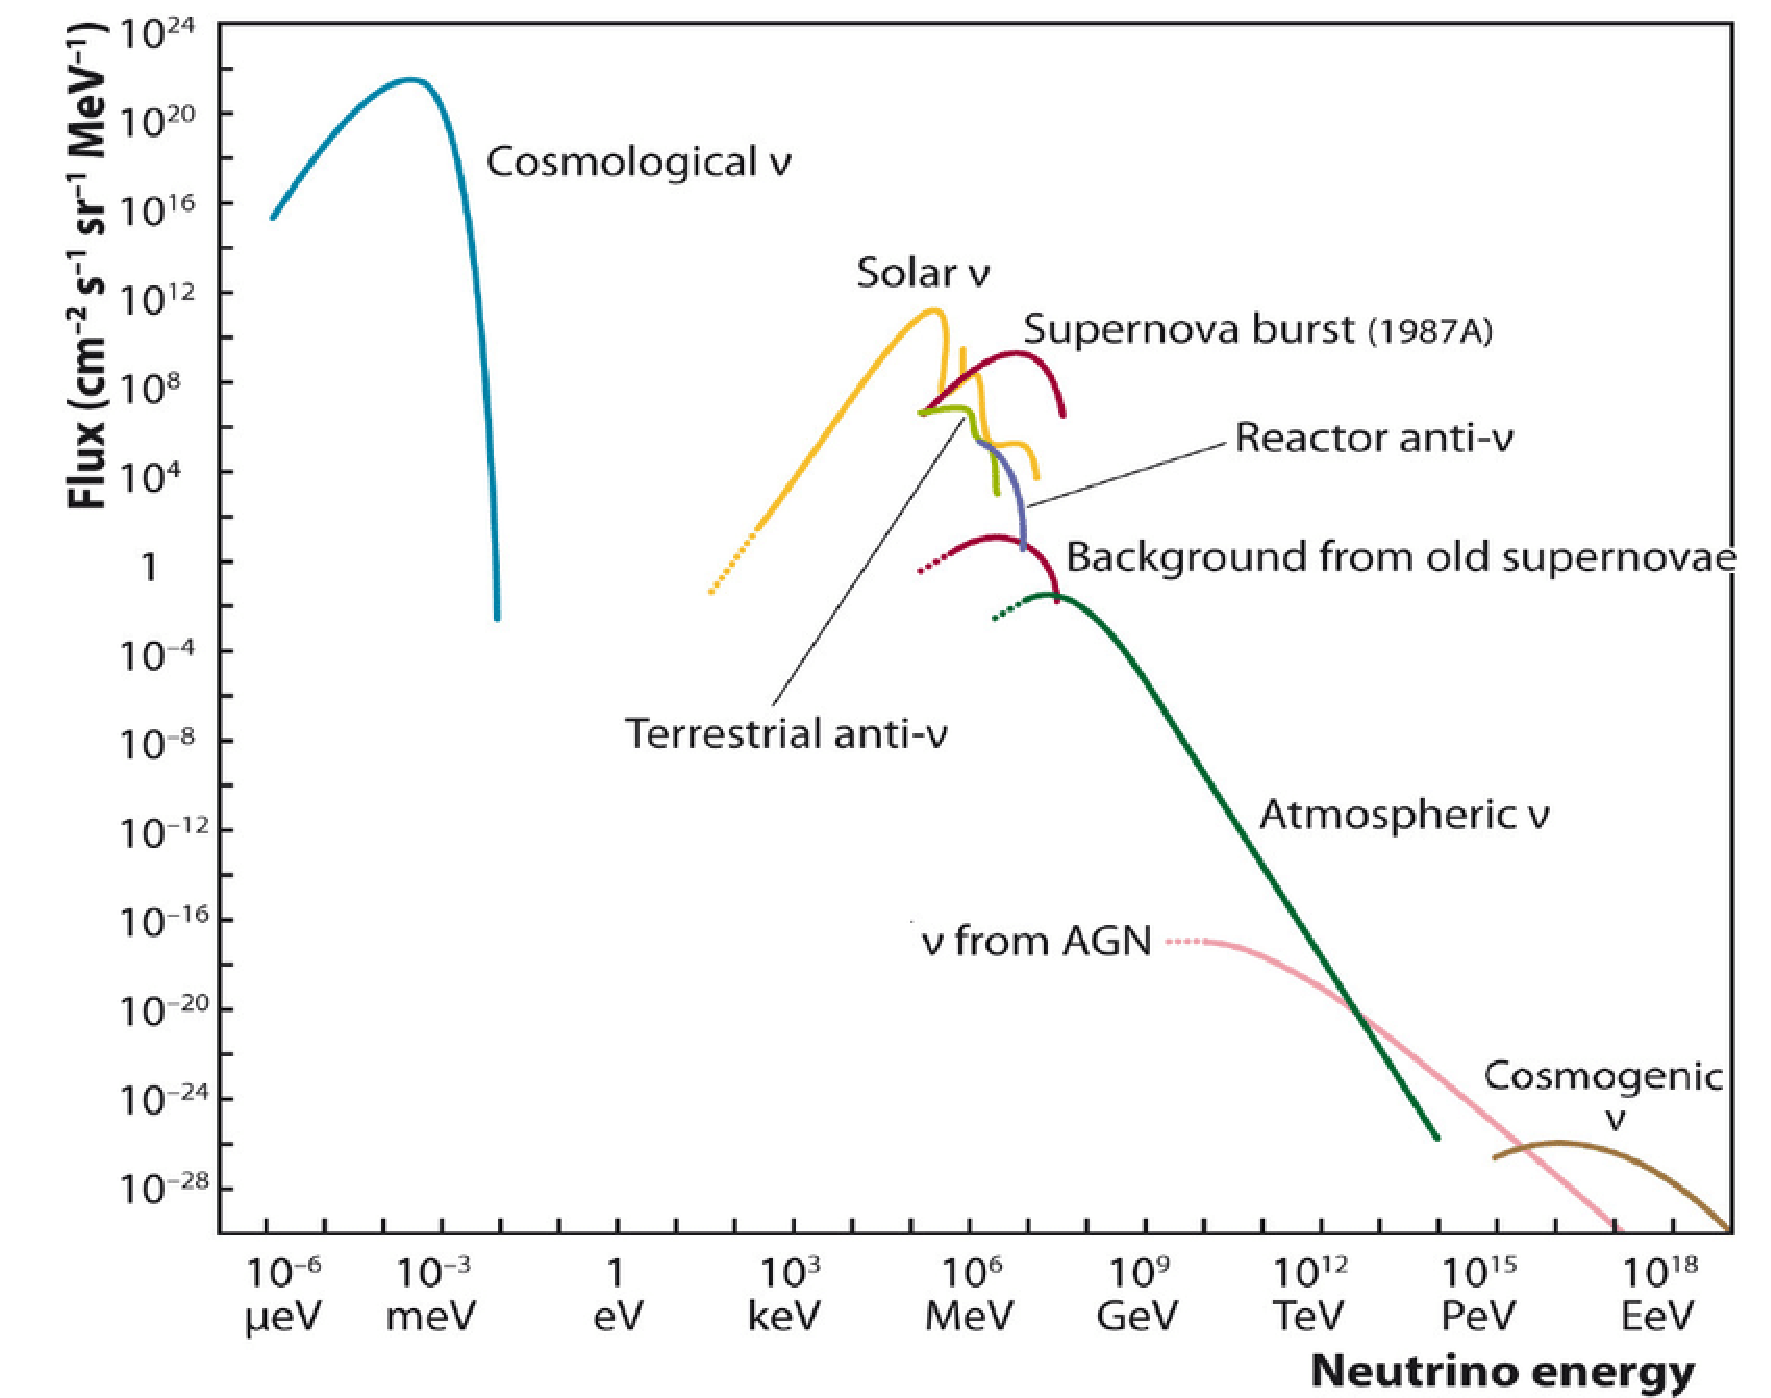
\includegraphics[height = 0.5\textwidth]{neutrinofluxes.pdf}}{\textcopyright Abhik Jash, Studies on the Physics of Resistive Plate Chambers in Relation to the INO Experiment}
	\caption{Predicted neutrino flux for various sources both natural and man-made}
	\label{figure:Neutrino fluxes}
\end{figure}
\subsection{Cosmological/Primordial neutrinos}
The first source of neutrinos we'll talk about is the one in blue to the left of the figure
termed the \textit{Cosmological neutrinos}: 
the neutrino version of the CMB.
To understand this source we'll have to go back all the way to just after the big bang:
The very early universe was hot and dense. As a result, interactions among particles
occurred much more frequently than they do today. As an example, a photon today
can travel across the observable universe without deflection or capture, so it has a
mean free path greater than $10^{26}$ m. When the universe was 1 second old, though, 
the mean free path of a photon was about the size of an atom. Thus in
the time it took the universe to expand by a factor of 2, a given photon interacted
many, many times. These multiple interactions kept the constituents in the universe
in thermal equilibrium. But as the universe expanded there were times when reactions could
not proceed rapidly enough to maintain equilibrium conditions, these particles then fall out
of thermal equilibrium. This falling out of equilibrium is termed \textit{decoupling}.
And we're interested in when neutrinos decoupled.
Neutrinos were kept in equilibrium through the interaction 
\begin{equation}
	\nu e \leftrightarrow \nu e
\end{equation}
up until the universe cooled down to about 1MeV when they decoupled.
To estimate the temperature of the neutrinos who decoupled at the start of the universe, 
we can take a look at conservation of entropy \cite{Dodelson} from which we'll find that
the temperatures are related by:
\begin{equation}
	T_\nu = \left(\frac{4}{11}\right)^{1/3}T_\gamma
\end{equation}
Note that they decoupled before the photons making them lower in temperature.
As $T_\gamma$ is the CMB temperature which, nowadays, is measured to be around
2.7K or $2.3\times10^{-4}$MeV. This would imply $T_\nu = 1.66\times 10^{-4}$MeV which
is roughly where the peak flux is located.  These primordial neutrinos are thus very
low in energy.
\subsection{Solar neutrinos}
The sun fuses elements to release energy and thus keeping itself from collapsing in 
on itself, with most of the various ways particles get fused, neutrinos get released as 
is shown in figure \ref{fig:SunFusion} where the neutrinos are electron neutrinos.
\begin{figure}
	\centering
	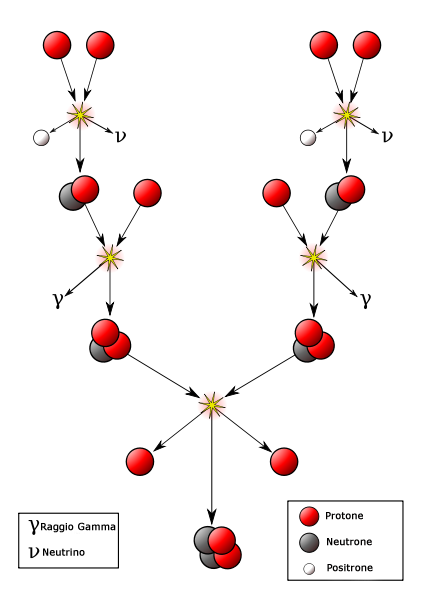
\includegraphics[width=0.4\textwidth]{figures/SunFusion.png}
	\caption{illustration of the full fusion cycle in the sun}
	\label{fig:SunFusion}
\end{figure}
Now with this and some information about the sun like the pressure and mass,
the \textit{standard solar model} was made. This model predicted a certain
amount of electron neutrinos to be hitting the earth from the previously mentioned
thermonuclear fusion, it was however 3 times higher than the observed amount of
electron neutrinos back at our planet. This led to a little bit of hysteria as this could've meant
that the sun was dying and we'd see the aftermath only in a couple of years.
Through various experiments however, it became apparent that this was due to
the different kinds of neutrinos oscillating into each other on their way to
earth, i.e 2/3 of the original electron neutrinos had oscillated into mu and
tau neutrinos. But for them to oscillate into eachother, they not
only require mass but each flavor also should have a different mass as can be seen
from an example 2D approximation to the transition probability\cite{Bellini_2014}:
\begin{equation}
	P(\nu_e\rightarrow\nu_\mu) = |\braket{\nu_\mu|\psi(L,T)}|^2 = c_\mu c_\mu^* = \sin ^2(2 \theta) \sin ^2\left(\frac{\Delta \phi_{12}}{2}\right)
\end{equation}
with
\begin{equation}
	\Delta \phi_{12} \approx \frac{m_1^2 - m_2^2}{2p}L
\end{equation}
In full generality (3D):
\begin{equation}
	\ket{\nu_\alpha} = \sum_iU_{\alpha i} \ket{\nu_i}
\end{equation}
With $U_{\alpha i}$ the Pontecorvo-Maki-Nakagawa-Sakata (PMNS) matrix.  This
phenomenon has been experimentally verified e.g through the descrepency from
the observed and expected neutrino events coming from a nuclear reactor \cite{Eguchi_2003}.
\subsection{Supernovae}
\label{sec:supernovae}
A star starts its life as a ball of pure hydrogen. At the core, due to the
gravitational pressure of the outside plasma, fusion of hydrogen into deuterium
and helium happens. Thus converting mass into energy. The pressure of this energy
counteracts the pressure of gravity and the star is stable.

When the hydrogen at the core runs out no more hydrogen can be fused. For stars
with masses between $8M_\odot$ and $30M_\odot$ ($M_\odot$ being the mass of the sun)
the fusion of heavier elements starts, this can't keep going on however as at
some point the star starts to form the most stable element: iron. 

It costs energy
to both make lighter elements than iron and heavier ones as can be seen on
figure \ref{fig:BindingEnergyCurve}.
\begin{figure}[!ht]
	\centering
	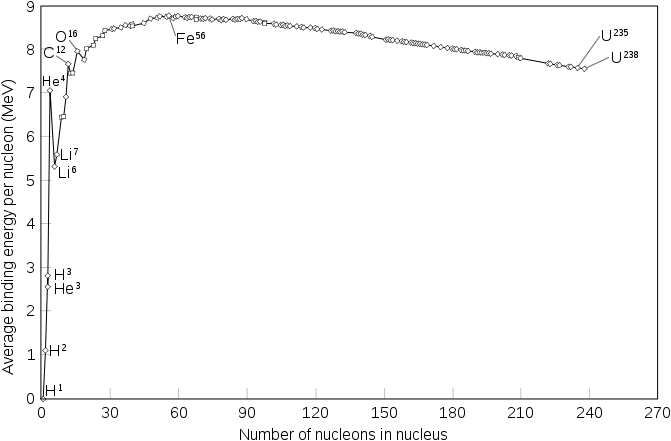
\includegraphics[width=0.5\textwidth]{Binding_energy_curve.png}
	\caption{Energy curve showing that iron is the most stable atom}
	\label{fig:BindingEnergyCurve}
\end{figure}
  As the iron core builds up the outside
pressure from the core starts to decrease as no new energy is released. This
goes on until  the treshold of an iron core with a mass of 1.4$M_\odot$ known
as the Chandrasekhar limit is reached and the the inwards pressure becomes too
large compared to the outwards pressure, making the electrons surrounding the
iron core fuse with the protons (uud), creating neutrons (udd) and neutrinos,
diagramatically shown in figure
\ref{fig:CoreFusion}.
\begin{figure}[h]
	\centering
	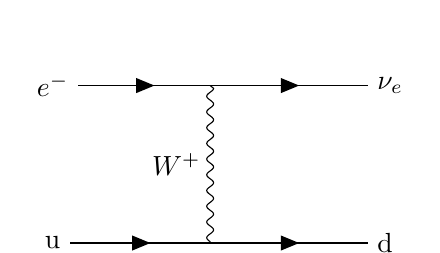
\begin{tikzpicture}
	\begin{feynman}
	\vertex (a0){u};
	\vertex[right=2cm of a0] (am) ;
	\vertex[right=2cm of am] (a1) {d};
	\vertex[above=2cm of am] (bm);
	\vertex[above=2cm of a0] (b0){$e^-$};
	\vertex[right=2cm of bm] (b1){$\nu_e$};
	\diagram* {
		{[edges=fermion]
			(a0) -- (am) -- (a1)
		},
		{[edges=fermion]
			(b0) -- (bm) -- (b1)
		},
		{[edges=boson,edge label=$W^+$]
			(am) -- (bm)
		}
	};
	\end{feynman}
	\end{tikzpicture}
	\caption{fusion of protons with surrounding electrons into neutrons via charged current exchange}
	\label{fig:CoreFusion}
\end{figure}\\
This last part happens in a split second as the collapse goes at 25\% the speed
of light, creating a very dense neutron star (3000km in diameter iron core to
30km in diameter neutron star) and up to $10^{52}$ ultra-relativistic
neutrinos, carrying up to 99\%\footnote{$\approx$1\% is released as kinetic energy, only 0.001\% as
electromagnetic radiation} of the released energy
\cite{Melson_2015}. As the density has suddenly increased so much
there's a huge distance of pure vaccuum between the plasma outer layer and the
(now) neutron star, this plasma starts free-falling inwards, also at 25\% the
speed of light whilst the neutrinos carrying tremendous amounts of energy start
going outwards from the neutron stars core.

The neutrinos then collide with the plasma resulting in what we observe as a
"supernova", wrongly thought of by Kepler as being a "new (nova) star" rather
being a violent death of an old star.

This is quite unexpected as neutrinos rarely interact, it's only as the
incoming plasma is so dense and due to the tremendous amount of neutrinos that
collissions happen at all. Some, however, escape and will be visible on earth
in our neutrino detectors $\approx$ 18h before the light escapes the exploding
star.

Neutrino observatories are thus also useful to know where to point our various
telescopes before the supernova is actually visible in the night sky.
\subsection{Background from old supernovae}
Also termed the \textit{diffuse supernova neutrino background} (DSNB), as the
universe is quite old various supernovae have happened over it's lifetime, each generating
a lot of neutrinos as was discussed in section \ref{sec:supernovae}. 
This is postulated to have generated a continuous neutrino background.
\subsection{Atmospheric neutrinos}
\label{sec:AtmosphericNeutrinos}
Before we can talk about atmospheric neutrinos it's necessary to discuss \textit{cosmic rays}.
Cosmic rays are ionized nuclei of which 90\% are protons, 9\% are alpha particles and
the rest are heavier nuclei. Almost all of them originate from outside the solar system but
from within our galaxy, the few particles that do come from our solar system can be temporally
linked to violent events on the sun. In contrast to this the particles coming from outside
our solar system show an anti-correlation with the sun as they can more easily reach the earth
if solar activity is low.
It has been observed that they roughly follow a power-law spectrum 
$N \propto E^{-\gamma}$ \cite{gaisser_engel_resconi_2016}.

Cosmic rays hit the Earth's atmosphere at a rate of about 1000 per square meter
per second and interact with atomic nuclei in the Earth's atmosphere, creating
showers of particles, many of which are unstable and produce neutrinos when
they decay, these neutrinos are what's called \textit{Atmospheric neutrinos}.
Most notably neutrinos can be produced together with muons in the two-body
decays of charged pions and kaons wherever these hadronic interactions occur.
The most important production channels and their branching ratios for neutrinos
are:
\begin{align}
	\pi^\pm &\rightarrow \mu^\pm + \nu_\mu(\bar{\nu}_\mu) (\sim 100\%)\\
	K^\pm &\rightarrow \mu^\pm + \nu_\mu(\bar{\nu}_\mu) (\sim 63.5\%)
\end{align}
Neutrinos are subsequently also produced when these muons decay:
\begin{equation}
	\mu^\pm \rightarrow e^\pm + \nu_e(\bar{\nu}_e) + \bar{\nu}_\mu(\nu_\mu)
\end{equation}
which is a process mainly happening at low energies in the atmosphere.  The
atmospheric neutrino spectrum shown in figure \ref{figure:Neutrino
fluxes} roughly follows a power spectrum as the cosmic ray flux follows a power
spectrum but the correspondence isn't one-to-one as, due to the difference in
kinematics, the contribution from kaons to neutrinos is significantly more
important than to muons, especially at high energies.

\subsection{neutrinos from AGNs}
An AGN (active galactic nucleus) is deemed to be the reason why several abnormal galaxies exist with
an extra bright (and mostly variable) light source in their core which even the biggest of telescopes
can't spatially discern. The general concensus is that this phenomenon is caused by one particular
kind of object: a supermassive black hole (a black hole with a mass of at least 105M$_\odot$) surrounded with
a close torus of dust and gas.
This torus of gas is called an \textit{accretion disc} and is an enormous source of energy. The conversion
of potential energy of the incoming gas to highly energetic radiation is a very complex physical process
with which we have to account for various factors like gravitational instabilities, magnetic fields, hydrodynamical
turbulence,... And thus produces a spectrum that's quite complex.
It would appear that the luminocity of an AGN would increase indefinitely with incoming mass, but this process is 
limited: if too much matter accretes on the black hole the radiative pressure becomes too massive and the 
matter on the disc gets blown away, this phenomenon is termed a \textit{black hole outburst}.

The emission of high energy neutrinos from AGNs rests solely on the premise
that relativistic protons of sufficiently high energy and energy density in the
AGN's accretion disc will be present \cite{NASANeutrinos} as they may interact
to create e.g pions whom decay into neutrinos. A direct consequence of the occurence of these
relativistic protons is the production of $\gamma$-rays of similar energies to
those of the neutrinos, thus high energy neutrino- and $\gamma$-ray astronomy are
closely related.  However, even though $\gamma$-ray photons can be produced
even in the absence of relativistic protons (e.g via high energy electrons),
neutrinos can not.  Thus the detection of these high-energy neutrinos (which
might have already been detected \cite{AGNNeutrino}) will provide unique
information about the workings of AGNs.
As these ultra high energy neutrinos get produced near the source (the AGN)
they are what's called \textit{astrophysical neutrinos}

\subsection{Cosmogenic neutrinos}
In contrast to the previous source of UHE neutrinos which was generated at the
source, called \textit{astrophysical neutrinos} we'll now talk about UHE
neutrinos whom are generated through the interaction of ultra-high energy
cosmic rays during propagation with the cosmic microwave or other photon
backgrounds termed \textit{cosmogenic neutrinos}.  The mechanism by which these
get created is quite simple, if a proton has sufficiently high energy the cross
section to interact with the CMB (Cosmic Microwave Background) becomes
non-negligable.  These protons can scatter off the photons to resonantly
produce a $\Delta^+$ baryon.  This resonance has enough mass to dominantly
decay to a pion and a nucleon:
\begin{align}
	\Delta^+ &\rightarrow \pi^0 + p \ \ (2/3)\\
	\Delta^+ &\rightarrow \pi^+ + n \ (1/3)
\end{align}
Of which the charged pion decays to neutrinos as previously mentioned in 
\ref{sec:AtmosphericNeutrinos}, these neutrinos carry most of the original energy.
\subsection{How do they fit into the full detector spectrum?}
The origin of the most energetic cosmic rays is still not conclusively
identified. One approach to solving this problem is \textit{multi-messenger
astrophysics}, where several types of cosmic particles are used to identify the
sources of these ultra-high energy cosmic rays (UHECRs). E.g we simultaneously
measure gravitational waves with the Einstein telescope, neutrinos with RNO-G,
photons with various telescopes and muons with a muon detector.
\newpage


\chapter{Radio neutrino detection}
\label{chap:RND}
In this chapter I'll explain how astrophysical neutrinos get detected in the
context of the Radio Neutrino Observatory in Greenland, or RNO-G.

Neutrinos are omnipresent in nature but as they interact very weakly we'll need
a big detector to detect reasonable amounts in finite timespans.  
To this end we can make use of a detector volume nature has
built for us: the Greenland icecap.  Even though various detector media
have been used, like water\cite{SuperKamio}, heavy water
\cite{SNO:1999crp} and
even the moon\cite{numoon}, ice has been chosen as it has a few properties which makes it easy to
work with, of which some are listed below:
\begin{itemize}
  \item Ice is mostly see-through for electromagnetic radiation in the radio-frequency range
  \item The Greenland icecap is a really big continuous volume with little to no background from human activity
  \item As it's really cold within the ice, the detectors don't have to be made water-tight (contrary
	  to in-water detectors)
  \item As ice is a solid the detectors are logistically easy to deploy
\end{itemize}

To detect a neutrino it has to generate some kind of signal. As will be
explained, neutrinos can interact with hadronic matter to produce charged
particles. For cubic-kilometer type in-ice detectors these charged particles can then
be detected through the Cherenkov effect in the visible spectrum or
through the Askaryan effect in the radio frequency range.
For RNO-G the Askaryan effect will be leveraged.

\section{Neutrino interactions in ice}
\label{sec:NIII}
As neutrinos propagate through ice they can interact weakly with the nuclei .
The main mechanisms of interaction is via charged- and neutral current exchange
(see section \ref{sec:WeakInt}) with the quarks\cite{NuRadioMc} as is also
depicted in figure
\ref{fig:NeutrinoNucleusInteraction}.
\begin{figure}[h!]
	\begin{minipage}{\textwidth}
		\begin{minipage}{0.49\textwidth}
			\centering
			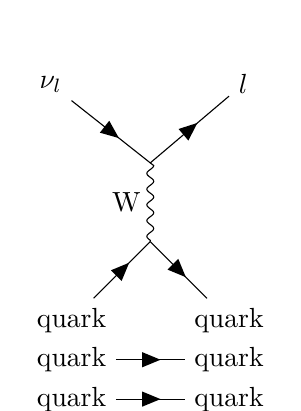
\begin{tikzpicture}
				\begin{feynman}
					\vertex (a0) {quark};
					\vertex[above=0.5cm of a0] (a1) {quark};
					\vertex[above=0.5cm of a1] (a2) {quark};
					\vertex[right=2cm of a0] (b0) {quark};
					\vertex[right=2cm of a1] (b1) {quark};
					\vertex[right=2cm of a2] (b2) {quark};
					\vertex[right=1.0cm of a2] (am);
					\vertex[above=1cm of am] (c0);
					\vertex[above=1cm of c0] (c1);
					\vertex[above=1cm of c1] (cm);
					\vertex[left=1cm of cm] (a3) {$\nu_l$};
					\vertex[right=1cm of cm] (b3) {$l$};
					\diagram* {
						{[edges=fermion]
							(a0) -- (b0)
						},
						{[edges=fermion]
							(a1) -- (b1)
						},
						{[edges=fermion]
							(a2) -- (c0) -- (b2)
						},
						{[edges=fermion]
							(a3) -- (c1) -- (b3)
						},
						{[edges=boson, edge label=W]
							(c0) -- (c1)
						},
					};
				\end{feynman}
			\end{tikzpicture}
		\end{minipage}
		\begin{minipage}{0.49\textwidth}
			\centering
			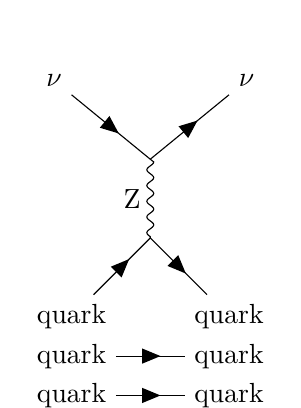
\begin{tikzpicture}
				\begin{feynman}
					\vertex (a0) {quark};
					\vertex[above=0.5cm of a0] (a1) {quark};
					\vertex[above=0.5cm of a1] (a2) {quark};
					\vertex[right=2cm of a0] (b0) {quark};
					\vertex[right=2cm of a1] (b1) {quark};
					\vertex[right=2cm of a2] (b2) {quark};
					\vertex[right=1.0cm of a2] (am);
					\vertex[above=1cm of am] (c0);
					\vertex[above=1cm of c0] (c1);
					\vertex[above=1cm of c1] (cm);
					\vertex[left=1cm of cm] (a3) {$\nu$};
					\vertex[right=1cm of cm] (b3) {$\nu$};
					\diagram* {
						{[edges=fermion]
							(a0) -- (b0)
						},
						{[edges=fermion]
							(a1) -- (b1)
						},
						{[edges=fermion]
							(a2) -- (c0) -- (b2)
						},
						{[edges=fermion]
							(a3) -- (c1) -- (b3)
						},
						{[edges=boson, edge label=Z]
							(c0) -- (c1)
						},
					};
				\end{feynman}
			\end{tikzpicture}
		\end{minipage}
	\end{minipage}
	\caption{Most prominent ways of neutrino-nucleus interaction}
	\label{fig:NeutrinoNucleusInteraction}
\end{figure}

The produced leptons in the W boson mediated interaction are either electrons,
resulting in an electromagnetic shower, muons which typically live
too long and thus escape the detector volume before they can deposit all of their 
energy in the ice\cite{PhdthesisWeling} or tauons which will decay via
\begin{equation}
	\tau^- \rightarrow e^- + \bar{\nu}_e + \nu_\tau
\end{equation}
or, less ideally
\begin{equation}
	\tau^- \rightarrow \mu^- + \bar{\nu}_\mu + \nu_\tau
\end{equation}
In both the charged and neutral current interaction, the resulting nucleus
will result in an hadronic shower. For the neutral current interaction
the fraction of the neutrino energy that gets transferred to
the nucleon is described by the inelasticity $y$ and is heavily shifted towards
small values of $y$\cite{elasticity_y}. This causes a big, irreducible
uncertainty when trying to estimate the original neutrino energy from these
kinds of events.  With the charged current interaction (mediated by the $W^\pm$
bosons) this isn't a problem however as the full neutrino energy ends up in the
resulting cascades.
\section{Askaryan effect}
\label{sec:Askaryan}
A particle shower in ice formed through the interactions described in section
\ref{sec:NIII} can emit strong radio signals if two conditions are met:
\begin{itemize}
	\item There is separation of positive and negative charges in the shower front 
	\item The signals produced over the length of the shower profile overlap coherently.
\end{itemize}
The \textit{Askaryan} \cite{Askaryan} effect, which is responsible for the
production of Askaryan radiation describes the effect at radio frequencies
which abides by both of these conditions.  In general it's a quite involved
effect but we'll give a crude overview. After neutrinos interact in the ice
they produce a cascade of secondary charged particles containing a net negative
charge anisotropy\cite{Connolly_2017}.  This charge imbalance is a result of
medium electrons either Compton scattering into the advancing shower or
annihilating with shower positrons.  This moving charge anisotropy is
propagating faster than the speed of light in the dielectric medium, creating
Cherenkov radiation.  

Cherenkov radiation can be considered the electromagnetic equivalent of a sonic boom. 
A sonic boom happens when an object goes faster than the speed of sound in the
medium; In the same way a particle emits Cherenkov radiation if it propagates faster than 
the speed of light in the medium.  Choosing the particle trajectory to lie along the z
axis an approximate equation can be found\cite{jackson1998classical} for
$\frac{\text{d}^2 \mathscr{J}}{\text{d}\omega \text{d}\Omega}$, which is the energy
radiated per elementary unit solid angle and per elementary unit frequency
interval:
\begin{equation}
	\frac{\text{d}^2 \mathscr{J}(\omega)}{\text{d} \omega \text{d} \Omega} = \frac{q^2}{4\pi}\sqrt{\frac{\mu}{\epsilon}}\beta^2\omega^2\delta^2[\omega(1-\beta \mathbf{e}_r\cdot\mathbf{e}_z)]|\mathbf{e}_r\times\mathbf{e}_z|^2 \label{equation: 4.128 in elektromagnetisme}
\end{equation}
Now we can re-write this equation in spherical coordinates, which gives $1-\beta \mathbf{e}_r\cdot\mathbf{e}_z = 1-\beta\cos(\theta_c)$ in the delta function. We thus only expect radiation if
\begin{equation}
\cos(\theta_c) = \frac{1}{\beta} = \frac{c'}{u} = \frac{c}{n}\cdot\frac{1}{u}
\end{equation}
With u the local speed of light in the medium and n the index of refraction, an optical
property of a medium which we'll later on thoroughly discuss.
If $u>\frac{c}{n}$, Cherenkov radiation will
be emitted along a cone surface with half angle $\frac{\pi}{2}-\theta_c$ as
illustrated in figure \ref{figure: Cherenkov illustratie}. Integrating equation
\ref{equation: 4.128 in elektromagnetisme} over the solid angle and formally
dividing by the time interval we get:
\begin{equation}
	\frac{\text{d}^2\mathscr{J}}{\text{d}\omega \text{d}t} = \frac{q^2}{4\pi}\sqrt{\frac{\mu}{\epsilon}}\beta\omega\left(1-\frac{1}{\beta^2}\right)	
\end{equation}
We see that the energy is proportional to $\omega$, so we expect that most
radiation will be emitted "in blue" with a cut-off frequency above which the
equation $\cos\theta = 1/(n\beta)$ can no longer be satisfied. This "in blue"
characteristic is responsible for the blue glow seen in nuclear reactors as
seen in figure \ref{figure: Cherenkov reactor} .  For ice the index of
refraction is roughly 1.78 in deep ice\cite{Bogorodsky1985}\cite{indexofrefrvalue}, 
so we expect an ultra-relativistic
particle to produce the most radiation at around 56° opening as 
\begin{equation}
	\cos(\theta_c) \approx \frac{1}{n} \implies \cos^{-1}\left(\frac{1}{1.78}\right)\approx 56\text{°}
\end{equation}
\begin{figure}
\centering
\begin{minipage}{0.45\textwidth}
	\centering
	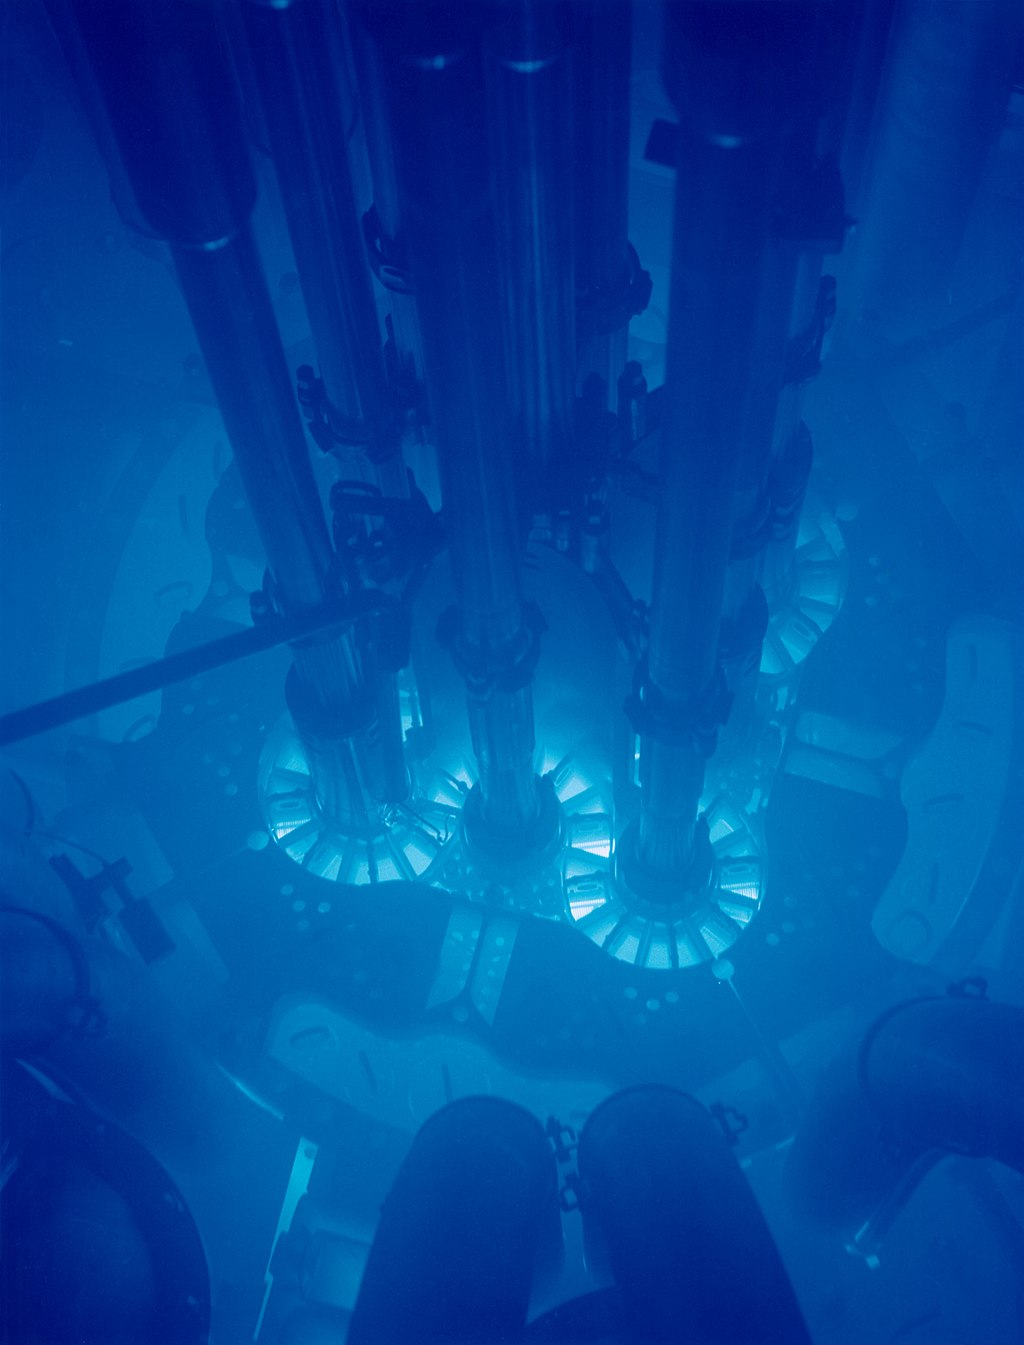
\includegraphics[height = 0.8\textwidth]{Cherenkov-reactor.jpg}
	\caption{The particles coming from the reactor core produce cherenkov radiation as they pass through the water,
	most of the produced light is "in blue"\citeFig{CherenkovReactor}}
	\label{figure: Cherenkov reactor}
\end{minipage}
\hspace{0.05\textwidth}
\begin{minipage}{0.45\textwidth}
	\centering
	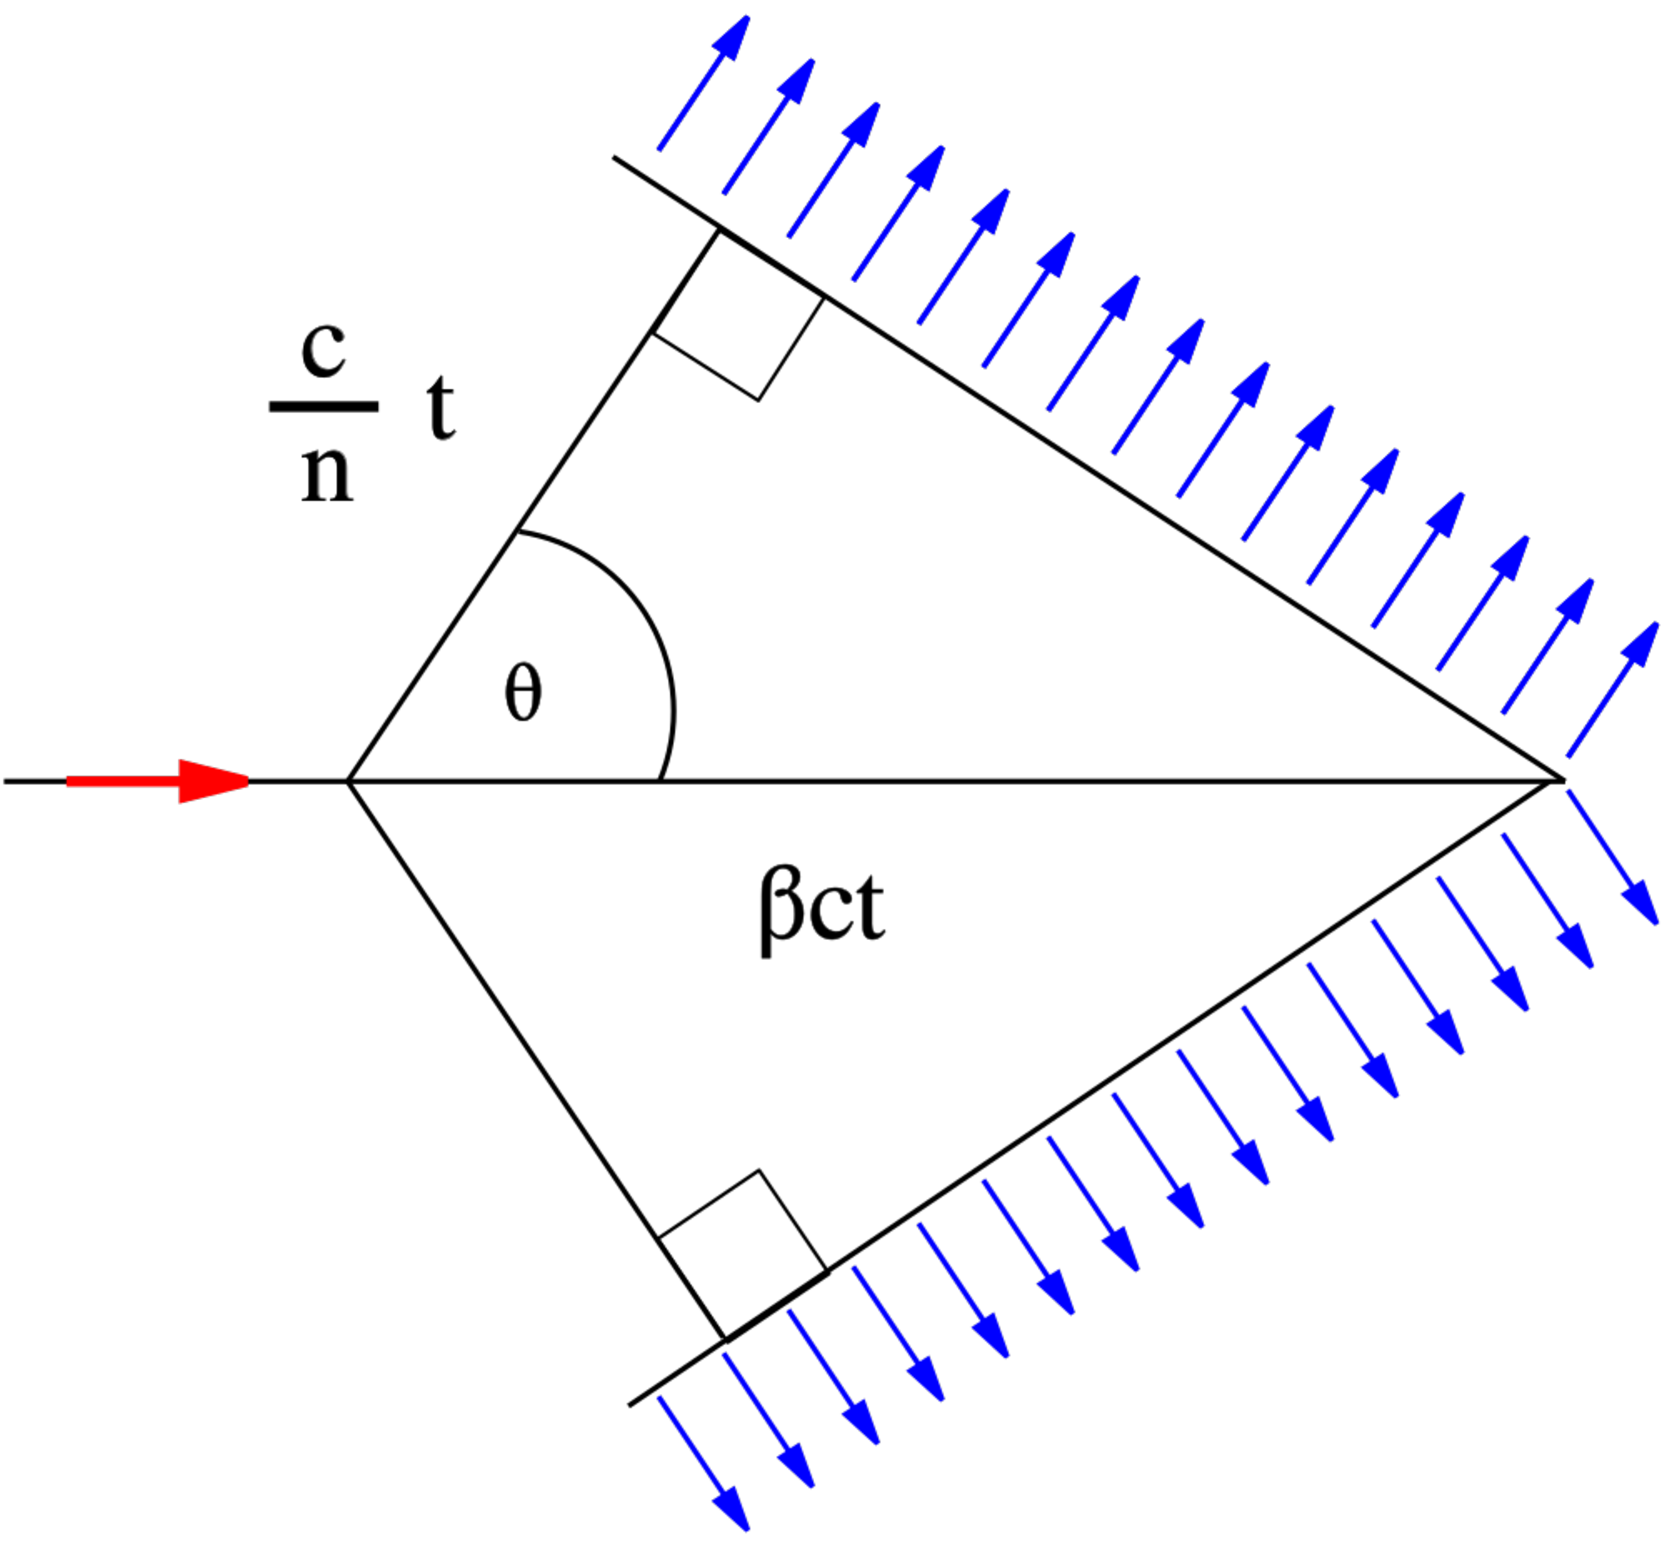
\includegraphics[height = 0.8\textwidth]{Cherenkov.pdf}
	\caption{The cone shape is reminiscent of a sonic boom, the signal is the strongest on the cone \citeFig{CherenkovIllu}}
	\label{figure: Cherenkov illustratie}
\end{minipage}
\end{figure}
Of course this is just an estimate, as the actual index of refraction is depth-dependent which
we'll get to in section \ref{section:Ice Model}.
Now this explains how the signals get generated but logically, from only knowing this
we'd expect radio waves to almost be non-existent 
due to the "in blue" nature of Cherenkov radiation. 

To understand why this isn't the case we'll need another piece of the puzzle: coherent overlap.
Coherent overlap in the radio wave spectrum range can be intuitively explained as
follows: generally the shower is of length
$\mathcal{O}$(10cm)\cite{Huege_2017}, over this length the radiation gets
emitted, most frequencies decoherently interfering, but radio waves with wavelengths of 
$\approx$ 10cm coherently interfere, and it's these waves we then wish to detect.
The radiation generated trough this Askaryan effect is called \textit{Askaryan radiation}.

The Askaryan radiation is polarized perpendicular to the Cherenkov cone, this
concept is illustrated in 2D in figure \ref{fig:illupol}.
The fact that the radiation is polarized can be useful to discern which
direction the neutrino came from using both vertically and horizontally
polarized antennae.
\begin{figure}
	\centering
	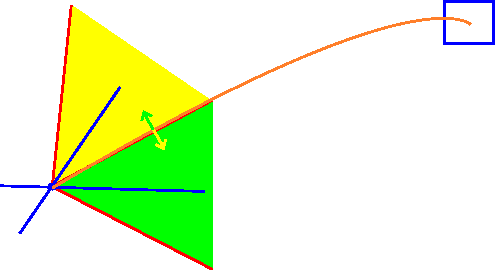
\includegraphics[width=0.5\textwidth]{illu_polarization.pdf}
	\caption{The detector receives an upwards polarization for the cherenkov cone in green
	and a downwards polarization for the one in yellow}
  	\label{fig:illupol}
\end{figure}

The radio signals that get produced by a neutrino interaction in ice always
travel along two paths, an example path is shown on figure \ref{fig:DnR}.  In
this figure the paths are direct and refracted, designated DnR, but note that
direct and reflected (at the surface) and refracted refracted are also
possible.
\begin{figure}
  \centering
  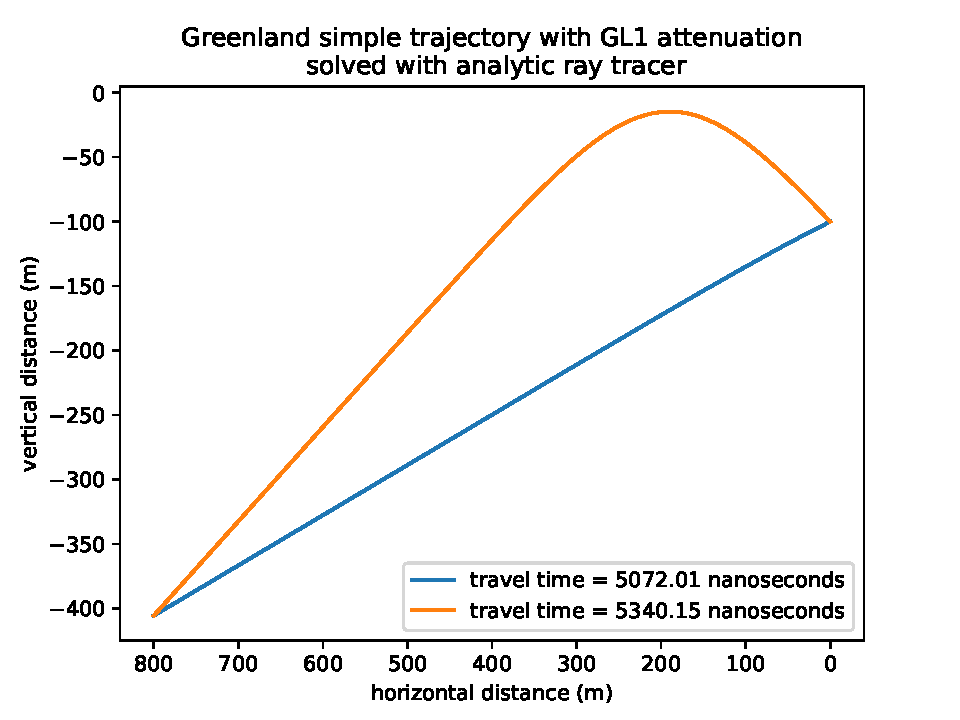
\includegraphics[width=0.7\textwidth]{DnR.pdf}
  \caption{example simulation showing both direct and refracted path from a neutrino vertex (bottom left) to a detector (top right)}
  \label{fig:DnR}
\end{figure}
This double pulse characteristic would be a smoking-gun signature of an in-ice
source.
\section{RNO-G}
Both cosmic ray and neutrino detectors face the same main problem at the
highest energies: the steeply falling flux (as was previously seen in figure
\ref{figure:Neutrino fluxes}) requires large effective areas, which leads to
the construction of neutrino detectors with volumes on the cubic kilometer
scale like IceCube\cite{IceCubeTechnical} which works on the principle of
detecting neutrinos with visible light.  But even IceCube has it's limitations,
it's still too small to observe many neutrino events above the 10 PeV
scale\cite{IceCubeGen2} in acceptable timescales. That's why a new detector was needed which was even
bigger and able to observe cosmogenic neutrinos.  We could just make IceCube
bigger but this would cost a lot of money as the individual detectors need to
be spaced closely as the attenuation length is quite short for light in the
visible spectrum propagating through ice.  

The proposed solution was to work with radio wave detectors, leveraging the
previously discussed Askaryan effect (see section \ref{sec:Askaryan}).  Radiowaves can propagate
way further in ice than visible light making it possible to space the
individual detectors further apart. The proposal was to build the detector in Greenland as shown in figure \ref{fig:GreenlandOP}. Greenand is an
island country in North America and part of the Kingdom of Denmark which has
large ice sheets making it a good candidate for radio neutrino detectors.
\begin{figure}
  \centering
  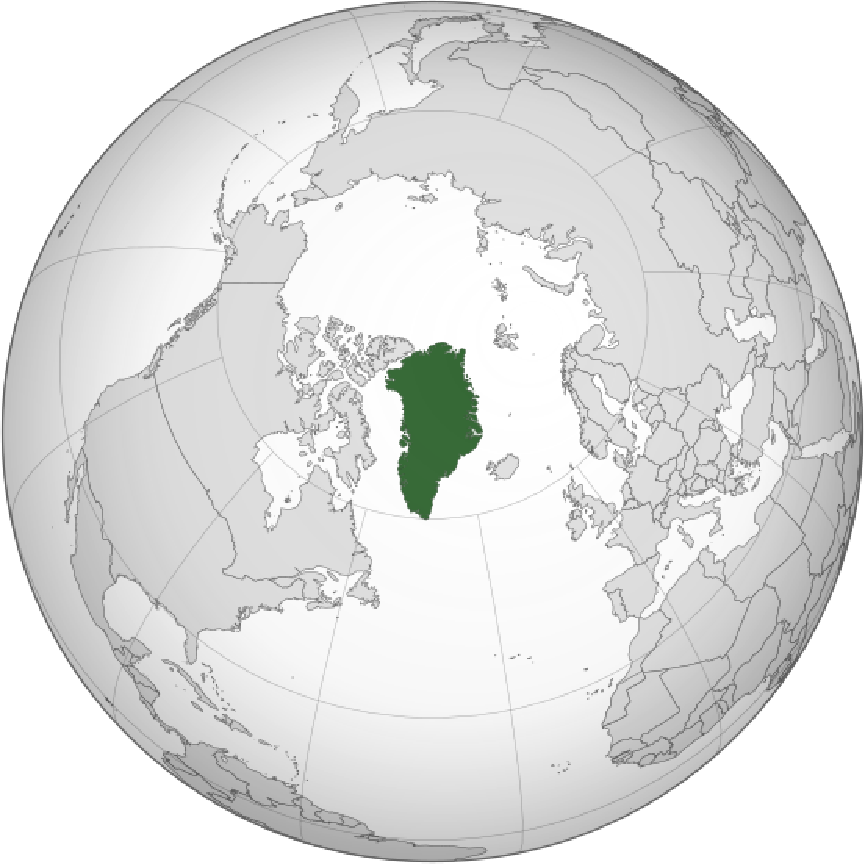
\includegraphics[width=0.5\textwidth]{figures/GreenlandOP.pdf}
  \caption{orthographic projection of Greenland with the red star representing the approximate RNO-G location\citeFig{OrthoGreenland}}
  \label{fig:GreenlandOP}
\end{figure}
The proposal for RNO-G, which was later funded and now in the construction
phase, is for it to be an array of autonomous radio stations each of which having both
surface channels and various deep channels resulting in a total of 24 channels
per station. The whole project builds heavily on the knowledge obtained through
previous radio based neutrino detectors like the NuMoon\cite{numoon} project,
ANITA\cite{ANITA}, ARA\cite{ARA},ARIANNA\cite{Barwick_2015} and RICE\cite{RICE}.

A station is illustrated in figure \ref{fig:detector}, 
\begin{figure}
	\centering
	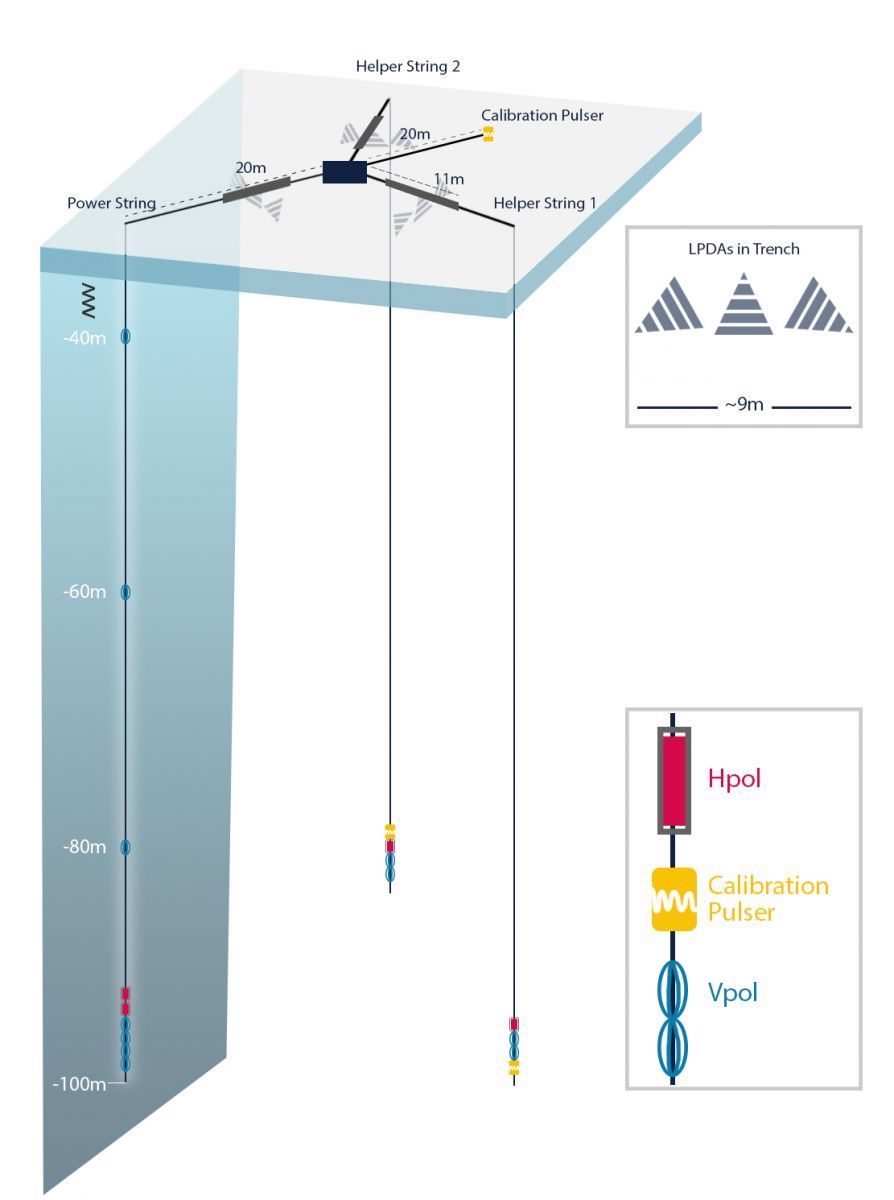
\includegraphics[height=0.4\textheight]{figures/RNO-G_station_sketch.jpg}	
	\caption{The combination of Vpol and Hpol antennae makes it possible to discern the direction of neutrinos whereas
	the surface LPDA antennae makes it possible to distinguish muons.\citeFig{DetectorIllu}}
	\label{fig:detector}
\end{figure}
the plan is to build 35 of these as is shown in figure \ref{fig:station map}. 
\begin{figure}
	\centering
	\includegraphics[width=0.55\textwidth]{figures/station-mapNoComment.png}	
	\caption{All the individual detectors are numbered but also named after various species living in
Greenland (in the native tongue)\citeFig{PlannedLay}}
	\label{fig:station map}
\end{figure}
Looking closely at one such detector we see
just below the surface 9 Log Periodic Dipole Antennas (LPDAs), these are used
to detect air shower muon signals as muons will also generate Cherenkov
radiation in the ice whose signals can then be filtered out.  Aside form these
surface detectors there are also deep components of the detector which can be
split up in three parts: Two \textit{helper strings} and the \textit{power
string}.

The helper strings are the 2 vertical cables shown on the right of figure
\ref{fig:detector} each housing 2 vertically polarized antennas (Vpols), one
quadslot antenna for the horizontal polarization component (Hpol) and one radio
pulser on each helper string which can be used to generate calibration signals.
As was previously mentioned using both the horizontal and vertical polarization of the
signal, the neutrino direction can be discerned. That's why both the helper and power 
string are equipped with both kinds of polarized antennae.

The power string (the leftmost vertical cable) is more densely instrumented
than the helper strings: At the bottom it houses a set of four Vpol and two
Hpol antennas with a spacing of 1m called the \textit{phased array}\cite{Allison_2019}. 
Due to the close spacing of the phased array it is possible to
interferometrically combine their signals creating a coherent receiver with a 
larger aperture than the individuals. This technique is frequently used in radio astronomy
for increasing the angular resolution by combining antennae and is the main
reason it was possible to observe the black hole Sagittarius A-star\cite{SqrA*}.
It is called the "phased" array as the radio array is electronically
steered using beamformers, which is called "phasing".
The resulting high resolution arguably makes the channels in the phased array the most important 
antennae of the detector.
Then finally further up the string, with a spacing of 20m, are three more Vpol antennas.
\begin{figure}
  \centering
  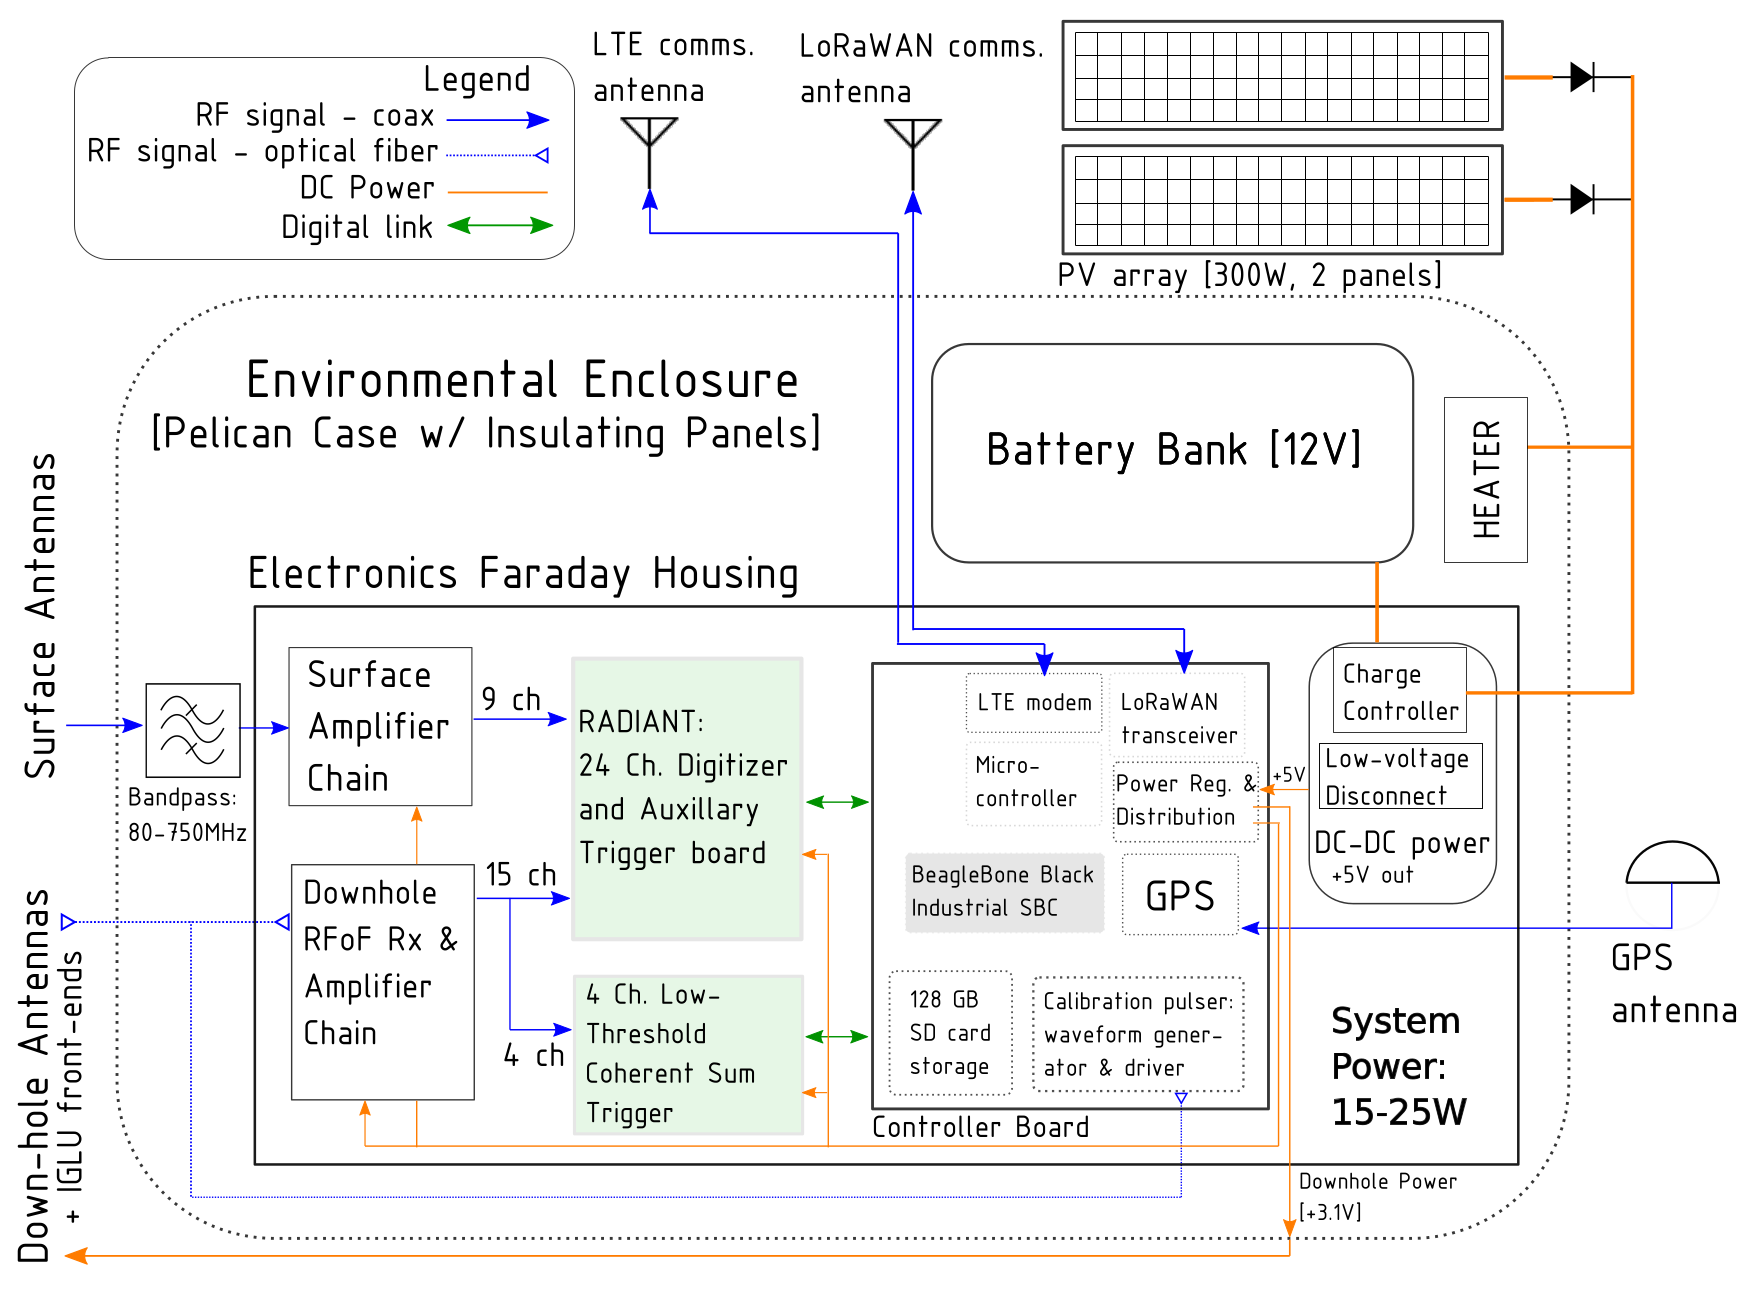
\includegraphics[width=0.85\textwidth]{SysDiagRNOG.png}
  \caption{System diagram for a RNO-G station \citeFig{Aguilar_2021_Fig}}
  \label{fig:SysDiag}
\end{figure}

A full system diagram for a RNO-G station is shown in figure \ref{fig:SysDiag},
We'll give a walk trough of how data gets collected.  The signal from each of
the deep antennae are fed into a low-noise amplifier directly above it\cite{Aguilar_2021}, from
there the signal is send to the data acquisition (DAQ) system at the surface
via a Radio Frequency over Fiber (RFoF) cable.  The signals coming from the
surface antennae are first passed through a Bandpass filter of
80-750MHz after which both the resulting signals and the deep component signals get sent
up to the RAdio DIgitizer and Auxiliary Neutrino Trigger (RADIANT). There it's
again amplified, digitized and, if a trigger threshold is reached, saved onto
an SD card. This data is then transmitted via a Long Term Evolution (LTE)
telecommunications network to a local server\footnote{There is additionally a
Long Range Wide Area Network (LoRaWAN) antenna as backup in case of problems
with the LTE network}, from where it is sent via a satellite link.
As a power source, battery banks are used whom are charged via solar panels.
But as there isn't enough light during the Greenland winters, there are plans to
build wind turbines (with one of the problems being the possibly detectable RF
noise the 'engine' would produce).

The two helper strings are needed for a full direction reconstruction.
Three independent measurements are needed for azimuthal information, which is
provided by the Vpol (Vertical polarization) antennas and placing the Hpol
(Horizontal polarization) antennas at different depths on every string, both
zenith and azimuth information will be provided for those signals. The helper
strings' calibration pulsers, as well as the one on the surface, will ensure
regular performance monitoring of the station and provide information
useful for precise calibration of the antenna geometry.

\section{Reconstruction}
When the channels pick up a signal which has a high enough amplitude to
cause it to trigger and record the data, how will it be analysed?

We can figure out wether the event was a neutrino or noise, where it came from
and it's energy using simulations. The code that's used to unravel the event
consists of 2 parts: NuRadioMC\cite{Glaser_2020} and
NuRadioReco\cite{Glaser_2019}. NuRadioMC uses Monte Carlo simulations to
generate neutrino events in the ice for particular energies and simulates how
they propagate to the various channels. This propagation will be covered more
in-depth in the next chapter.  NuRadioReco is reconstruction software, it
simulates how the various detectors would respond to the simulated incoming
radio waves.  Combining these two pieces of software thus makes it possible to
figure out how a signal looks like when a certain flavor of neutrino  
comes from a certain direction, interacting with the matter trough
either W or Z-boson exchange at a certain point in the ice with a certain
energy. 

How is this code then used to analyse an event?
A plan \cite{lookuptable} is to simulate a lot of neutrino events for various energies and
record the detector responses in a giant database, then, when an actual neutrino
event occurs, look in the database and match the actual
detector response to the simulated detector responses, thus finding the origin .

\section{Multi-Messenger Astronomy}
The origin of the most energetic cosmic rays is still not conclusively
identified. One approach to solving this problem is \textit{multi-messenger
astrophysics}, where several types of cosmic particles are used to identify the
sources of these ultra-high energy cosmic rays (UHECRs). E.g we simultaneously
measure gravitational waves with the Einstein telescope, neutrinos with RNO-G,
photons with various telescopes and muons with a muon detector.

As layed out in section \ref{sec:supernovae}, neutrinos from a supernova can
get observed on earth $\approx$18h before the visible light escapes the
supernova. To make use of this the Supernova Early Warning System
(SNEWS)\cite{SNEWS} was established, it can automatically give early warnings
to astronomers in the event of a supernova in the Milky Way, or a nearby galaxy
such as the Large Magellanic Cloud or the Canis Major Dwarf Galaxy.  Using this
SNEWS system astronomers can prepare by pointing their telescopes at the right
part of the sky prior to observing the event, thus being able to witness the
beginning in high resolution.

\chapter{Ray tracing}
\label{chap:RT}
As mentioned in the previous chapter, we want to simulate the signal a neutrino event
would produce in the detector. The neutrino event generates radiowaves that end
up at our detector, but as the ice has a continuously varying density, these radiowave
paths need to be computed.

In this chapter we'll go more in-depth as to how the radio wave paths get
simulated in ice within the NuRadioMC framework.
\section{Wave propagation}
\label{sec:WaveProp}
\begin{figure}[h!]
	\centering
	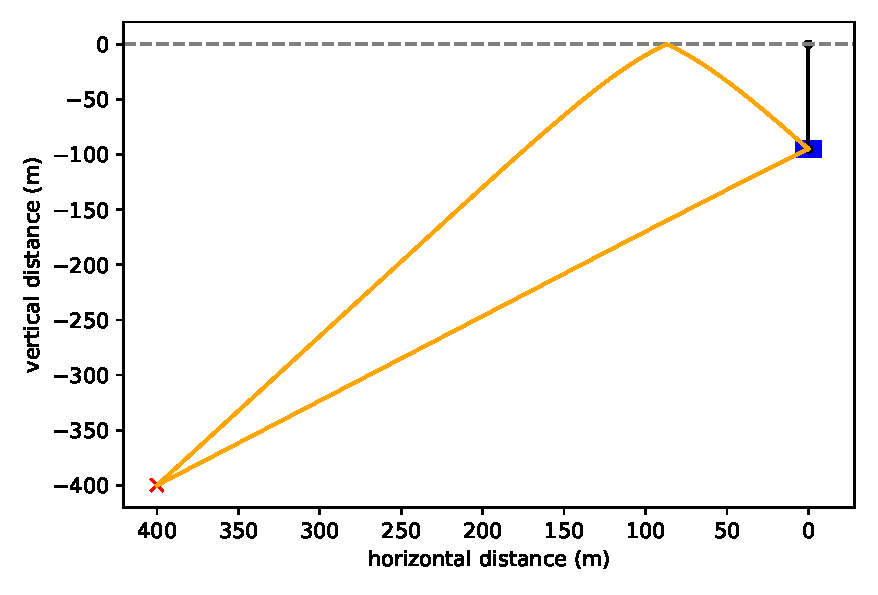
\includegraphics[width=0.7\textwidth]{DirectNReflected.pdf}
	\label{fig:PathIllu}
	\caption{Simulated radio wave paths from a source to a detector, these always come in a pair 
	if it's an in-ice source due to the density gradient of the ice and the reflective ice-air boundary.}
\end{figure}
There is a multitude of photons coming from our event but only the ones
in line with the cherenkov cone are strong enough to be detectable.
We thus only need to concern ourselves with simulating those.

The way we simulate the strongest waves propagating to the detector from a
radio source is through a process called ray tracing which we'll explain shortly, 
an illustration of the final result of ray tracing is shown in figure \ref{fig:PathIllu}.  

The amount of solutions (i.e how many radio wave paths exist between our source and the detector)
and how the waves are bent are consequences of the
properties of the ice we work in.  In a dielectric medium a ray propagates with
its signal wave-speed determined by the local index of refraction as $v =
c/n$. But the effect on speed isn't the only property the index of refraction has
which we'll need to concern ourselves with, another one is the breaking of the path,
but to understand that effect in continuous media we'll first need to talk about Snell's law. 

If a ray propagates towards a boundary dividing 2 media with different indexes
of refraction, the ray will refract and the refracted angle can be found from
Snell's law:
\begin{equation}
	n_i\sin{\theta_i} = n_o\sin{\theta_o}
\end{equation}
Where n is the index of refraction, $\theta$ the angle with respect to the
surface normal and "i" and "o" indicating incoming and outgoing respectively.
The system we'll consider however, isn't homogeneous with some specified
boundary. Ice in Greenland has a continuously varying density and
index of refraction.

How do we know how the waves propagate in such a medium?  The software we'll be
using to simulate how the radio waves behave is called \textit{Radiopropa}
\cite{Winchen_2019}. As simulations of the wave propagation in full detail with
the finite-differences-time-domain (FDTD) technique \cite{1138693} (solving
maxwells equations on a grid) are, even though they are more accurate, quite time
consuming. The authors of radiopropa opted to build their program on
geometrical optics, i.e ray tracing. A path of a ray $\mathbf{r}(s)$ with path
parameter s in a medium with index of refraction n($\mathbf{r}$) is described
by the eikonal equation\cite{herman2019treatise}:
\begin{equation}
	\frac{d}{ds}\left(n(\mathbf{r})\frac{d\mathbf{r}}{ds}\right) = \mathbf{\nabla} n
\end{equation}
in radiopropa the local paraxial approximation (small angle approximation) is
used, i.e if we assume that in any individual step of the algorithm the change
of the refractive index along the path $ds$ is small it's possible to rewrite
the equation as:
\begin{equation}
	n(\mathbf{r})\frac{d^2\mathbf{r}}{ds^2} \approx \mathbf{\nabla} n
	\label{eqn:radiopropaformula}
\end{equation}
Which is then numerically solved using the Cash–Karp method.  The way you would
go about using this program is thus: given a starting point (e.g a supposed
neutrino interaction point), "shoot" your ray in a
certain direction. Radiopropa will then compute the path the ray takes. 
If you chose your direction right, this ray will at some point cross an
"end point" you gave it (e.g the location of the detector) at which point it will
stop simulating. Meaning that you now have computed the path from a start point in ice
to an end point.

The difficulty in this matter is choosing the direction right so the ray
crosses paths with the end point, for this a wrapper algorithm is needed which we'll
get to later.  If there are boundaries (such as in-ice defects or the ice-air surface) these
are treated separately within radiopropa using Snell's law. 
\section{Ice model}
\label{section:Ice Model}
Radiopropa, as previously described, is based on solving equation \ref{eqn:radiopropaformula}.
This equation is dependent on the local index of refraction $n(\mathbf{r})$ for which
we'll thus need a model. But before we can derive a model we'll need to talk about the
density-depth relation.

Due to the way the ice bonds there will be more air trapped in between the
molecules closer to the surface than at greater depths where the pressure due
to the overhead ice prevents this.  Due to this air being trapped, the density
of ice will be smaller closer to the surface than at greater depth.  The region
where this air occurs in the ice is called the firn\cite{Firn} as to
distinguish it from glacial ice which is ice at large depths with nearly no air
trapped.

Purely from classical gravity and density considerations it can be derived that
the density scales exponentially. To see this let's consider a sheet of ice in
the Greenland firn with a surface A at a depth z and with a width dz, the extra
pressure this sheet of ice exerts on the ice just below it is:
\begin{equation}
	d\sigma = \frac{dF}{A} = -\frac{gdM}{A} = -g\frac{A\rho(z)dz}{A} = -g\rho(z)dz
\end{equation}
with $\rho(z)$ the depth-dependent density. The proportional change in air
space is assumed to be proportional to the change in
pressure\cite{herron_langway_1980}:
\begin{equation}
	\frac{dV}{V} \propto d\sigma
\end{equation}
As the volume scales inversely with the density let's assume the relation $V \propto (\rho_i - \rho)$ with
$\rho_i$ the density of pure ice, this yields:
\begin{equation}
	\frac{d\rho}{\rho_i - \rho} \propto \rho dz
\end{equation}
Which can be solved to give
\begin{equation}
	\rho = \frac{A\rho_i e^{z/z_0}}{1 + Ae^{z/z_0}}
\end{equation}
The following function was also empirically fitted:
\begin{equation}
	\label{eqn:myderiexp}
	\rho = \rho_0 e^{z/z_0} + B
\end{equation}
Figure \ref{fig:DensityMeasurements} shows how both of these functions fit the
density-depth data\cite{alley_koci_1988}\cite{hawley_morris_mcconnell_2008}.  
\begin{figure}
  \centering
	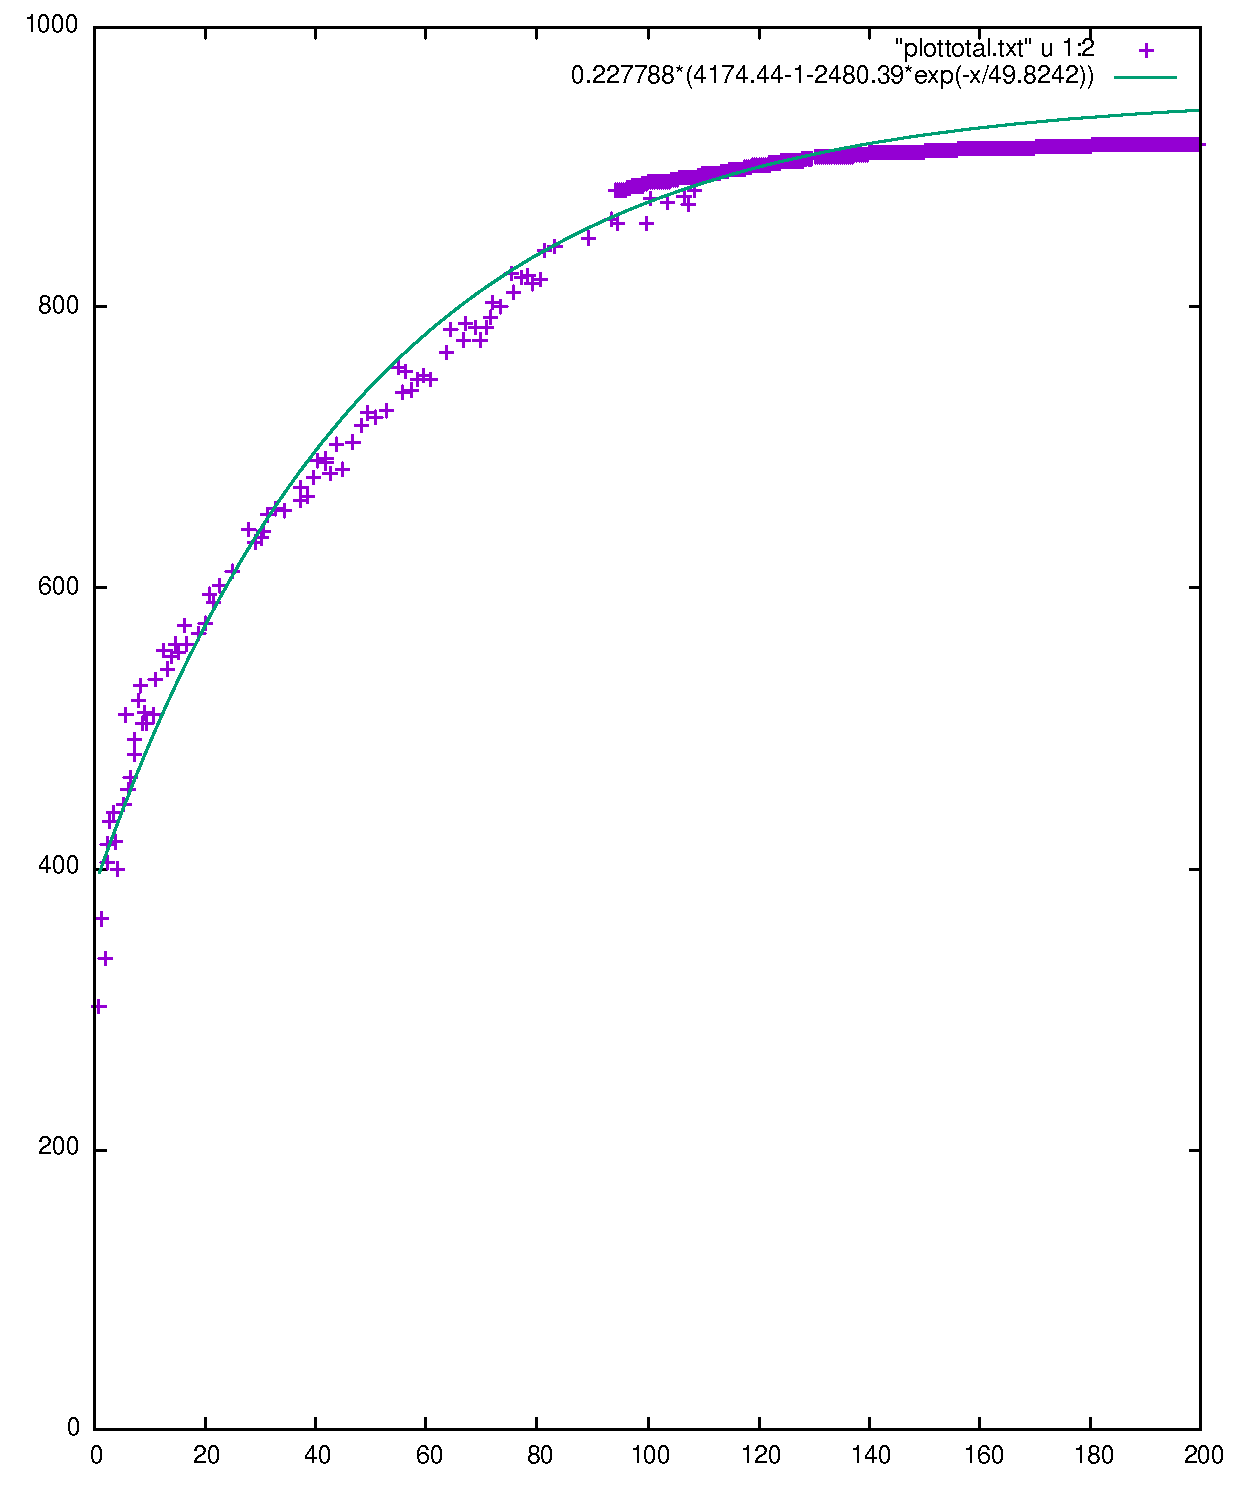
\includegraphics[width=0.5\textwidth]{Density_measurements2.pdf}
	\caption{Illustration of the shortcomings of the analytical models}
	\label{fig:DensityMeasurements}
\end{figure}
Now that we have a model for the density-depth curve we can link this to the
index-depth relation we need for radiopropa.  The dependence of the dielectric
constant on density for ice can approximately be given by\cite{Robin}:
\begin{equation} 
	\epsilon(z) \approx (1 + 0.845\rho(z))^2 
\end{equation} 
Here $\rho$ is called the \textit{specific gravity} as to make the equation
dimensionally correct, this is the same as the density in g/cm$^3$ but stripped
off its units.  As the dielectric constant is the square of the index of
refraction we can find an approximate index-density relation:
\begin{equation} 
	n(z) \approx 1 + 0.775\frac{\rho(z)}{\rho_0} \approx 1 + 0.78\frac{\rho(z)}{\rho_0} \label{eqn:Schytt}
\end{equation} 
Where we introduced $\rho_0$, the density for solid ice (917 kg/m³).  
Now that we have a linear relation between the index of refraction and the density
and also a model for the density-depth relation (equation \ref{eqn:myderiexp}) these two can
be combined to form the \textit{single exponential model}
\begin{equation}
	\label{eqn:expn}
	n(z) = n_{ice} - \Delta n e^{z/z_0}
\end{equation}
with $n_{ice}$ the refractive index of solid ice and $\Delta n = n_{ice} - n_s$
with $n_s$ the index of refraction of snow. 

Using this exponential model for radiopropa has a huge advantage as it's
analytically solvable, meaning that we can know which direction we'll have to
shoot our ray in after the location of the neutrino interaction and the
detector are specified. The ray tracing algorithm developed using this
exponential index is called the \textit{analytic ray tracer}.

\section{Shortcomings of the exponential ice model}
As can be seen from figure \ref{fig:DensityMeasurements}, there is a
discrepancy between the single exponential fit used for the exponential model
and the density data, especially between 40 and 120 meters of depth where the
phased array is located.  This discrepancy could imply that the analytic ray tracer will
make slightly wrong predictions.  This is why the development of a different
ray tracer was needed which will be able to handle more complex ice models. One
such ray tracer, called the iterative ray tracer, will be explained in section \ref{sec:Iterative} but this ray
tracer has its shortcomings. That's why we found that the development of a new ray tracer
was needed which is the partial work of this thesis and we'll get to that ray
tracer in chapter \ref{chapter:hybrid}.

\begin{figure}
  \centering
  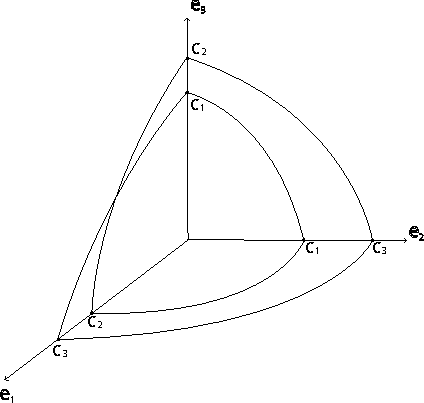
\includegraphics[width=0.5\textwidth]{figures/Fresnel.pdf}
  \caption{The three unit axes each have 2 possible wave speeds. E.g if a wave would
  travel along $\mathbf{e}_1$, depending on the polarization it could travel at a speed $C_3$ or
  at a speed $C_2$. The exponential model assumes all speeds to be the same, i.e $C_1=C_2=C_3=c/n$}
  \label{fig:Fresnel}
\end{figure}

There is also another effect worth mentioning that the exponential model
doesn't account for which might become important in the future: birefringence.
Up until now we have implicitly assumed that ice is isotropic meaning that both
its permittivity $\varepsilon$ and its permeability $\mu$ are scalars but
these could very well be tensorial in nature for radio waves in ice. In
general, after calculating this tensorial nature through you'd find that in
every direction two different indices of refraction can be found implying two
different types of waves each propagating with a different speed as illustrated
in figure \ref{fig:Fresnel}.  Of these two possible speeds in a direction, which the waves actually
follows is then dependent on the polarization of the wave, which in our case thus depends
on the Askaryan effect (see section \ref{sec:Askaryan}).  This optical property
coming from the anisotropic nature of the material is what's called
\textit{birefringence}.  Birefringence has been researched for it's
implementation into the simulation software NuRadioMC\cite{Heyer2023}.
\newpage
\section{Iterative ray tracer}
\label{sec:Iterative}
To work with more complex index-depth relations there's a need for a
new algorithm which is able to find the angle with which radiopropa should
shoot its ray if given the neutrino interaction and detector location.

To this end the iterative ray tracer \cite{2022icrc.confE1027O} was developed.
As can be derived from its name, it iteratively searches the path a ray might
take. We'll now explain the workings of the first part of the algorithm, a handy
accompanying illustration is given in figure \ref{fig:Illustration of iterative algorithm}.
\begin{figure}
  \centering
  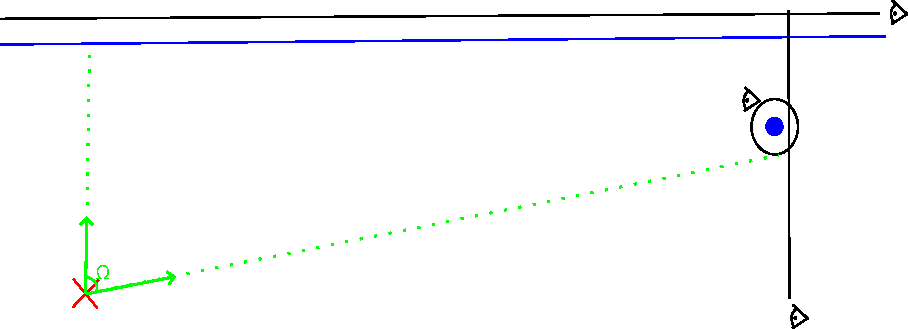
\includegraphics[width=0.8\textwidth]{algoillu.pdf}
  \caption{Illustration of the setup. The red cross is the neutrino interaction vertex, the blue dot is the detector,
  the observer sphere around the detector stops the simulation counting it as a solution and the other obervers (other lines with eyes) don't count the ray as a solution.}
  \label{fig:Illustration of iterative algorithm}
\end{figure}
\subsection{Setup}
Say we have a neutrino interaction point $\mathbf{X}_i$
(the red cross on the figure) and a detector located at $\mathbf{X}_d$ (the
blue dot on the figure), the algorithm starts by constructing an
\textit{observer} sphere with radius $r_1$ with the detector, located at $\mathbf{X}_d$, as the
center.  This means that any ray that gets shot and propagates to the sphere
will get stopped and counts as a solution.  Then, to reduce the time spent simulating, there are also observers placed
whose purpose is to stop the ray tracing but not count the observed signal as a solution.
One such observer is placed 
just above the ice surface as a ray that escapes the ice won't be able to make it back, and one
is placed just behind the detector looking from the point of the interaction vertex $\mathbf{X}_i$ as
a ray is not able to reach the detector anymore after it has passed it in the
lateral direction. 

Finally it's noted that due to the way the ice's index of refraction
continuously increases with depth, rays can't propagate upwards, this means that we only 
have to look for solutions within the angle $\Omega$ which is just the zenith angle the detector
makes with the bottom of the observer sphere.

\subsection{Narrowing algorithm}
Now that the setup has been established we'll just iteratively shoot rays from the neutrino
interaction point starting at an angle $\Delta \theta_1$ then at an angle
$2\Delta \theta_1$, $3\Delta \theta_1$,... Until we have reached $\Omega$. This
process is illustrated on the left side of figure \ref{fig:IterativeWorkings}.
\begin{figure}
  \centering
  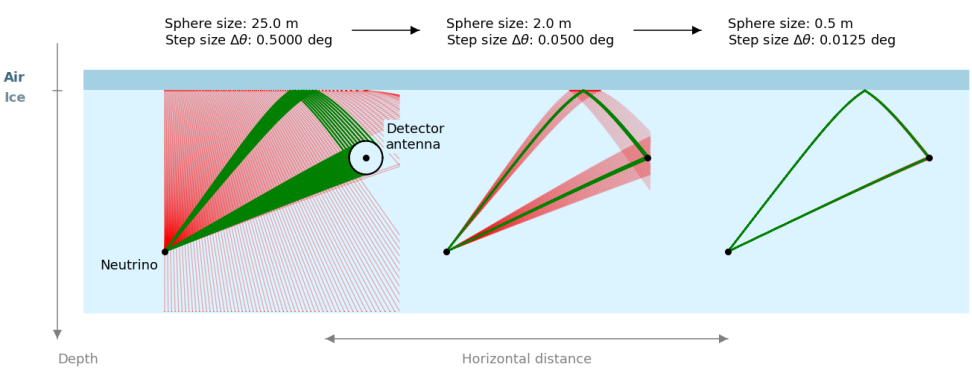
\includegraphics[width=0.9\textwidth]{IterativeWorkings.png}
  \caption{Illustration of the steps in the iterative ray tracer, first rays get shot in steps of 0.5°, the ones that end up at the sphere with a 25m radius are colored in green and within these angles the algorithm repeats (middle figure) but now with a smaller
  step and sphere size. \citeFig{2022icrc.confE1027O} }
  \label{fig:IterativeWorkings}
\end{figure}
After we have gone over all the different launch angles we'll have some
solutions (marked in green) and some that don't end up on the sphere around the detector (marked
in red) we can now make the observer sphere's radius smaller ($r_2 < r_1$) and
the step size of the angle smaller ($\Delta \theta_2 < \Delta \theta_1$).  And
again iteratively find the rays which end up on the sphere, only this time
looking within the angles of the solutions of the previous step. We can keep on
making the sphere and step size smaller in iterative steps until we've reached
the precision we want. We then take, for each bunch of solutions within an
angle interval, the most normal to the detector as the final solutions.




\chapter{Hybrid Ray tracer}
\label{chapter:hybrid}
%----------------------------------------------------------------------------------------
%	HYBRID RAY TRACER	
%----------------------------------------------------------------------------------------
Radio waves get simulated within the NuRadioMC framework via geometrical
optics, also known as ray tracing which we layed out in section \ref{sec:WaveProp}.
The ray tracing algorithm that's being used is radiopropa and is dependent on
the ice model. To simulate a path using radiopropa you need a start position 
and a launch angle, if you only have the initial and final position you'll need
a wrapper algorithm for determining the launch angle.  
A wrapper algorithm that works with complex ice models was developed previously
called the \textit{iterative ray tracer}\cite{2022icrc.confE1027O}, and was
discussed in section \ref{sec:Iterative}.

The way the iterative ray tracer works is sub-optimal as it uses it's own
procedure in python which in general will work slower and less accurate than an
optimization library. Work had been done on trying to implement an algorithm
using optimization libraries deemed the "minimizer", but this attempt failed as
there was no reliable way to determine initial launch angle intervals over
which to minimize.  As we saw this work the idea came to mind to combine the
iterative ray tracer and the code used in this minimizer. Inspired, we
built the algorithm which will be discussed in this chapter: The \textit{hybrid ray
tracer}, in the source code called the "hybrid minimizer" \cite{hybrid}. 

The hybrid ray tracer succeeds in more rapidly finding the path from the event
to the detector than the iterative ray tracer, is also more accurate and
arrives closer to the detector as the final result is not limited by the final
drawn sphere size but by a given tolerance making it useful for simulations in
which high time and space precision is needed like plane wave reconstruction,
which we'll do in chapter \ref{chap:WB}.

\section{How the hybrid ray tracer works}
The hybrid minimizer can be seen as an extension of the iterative ray tracer as
it starts out the same way, so to understand the first step I refer to section 
\ref{sec:Iterative}. Only the leftmost step of the three steps shown in figure
\ref{fig:IterativeWorkings} is completed, after this step two distinct launch regions
have been found.

After 2 distinct launch regions have been found, say in the regions
$[\theta_1,\theta_2]$ and $[\theta_3,\theta_4]$, 
then the so called \textit{minimization} procedure will
start. Using scipy's module optimize.minimize the optimal solution will be
found by using the Nelder-Mead method\cite{10.1093/comjnl/7.4.308}. First we
get rid of the spherical observer and place the vertical observer at the
detector, now to be able to use the minimize module we'll need a function to
minimize, for this reason we first define the function \textit{delta\_z} as,
given a certain launch angle, propagating the ray onto the vertical observer
and returning the distance from the point where it lands on the plane to the
detector, as illustrated on figure \ref{fig:PrincipleHybridIllu} (i.e it
returns the value $\Delta z$).
\begin{figure}
  \centering
  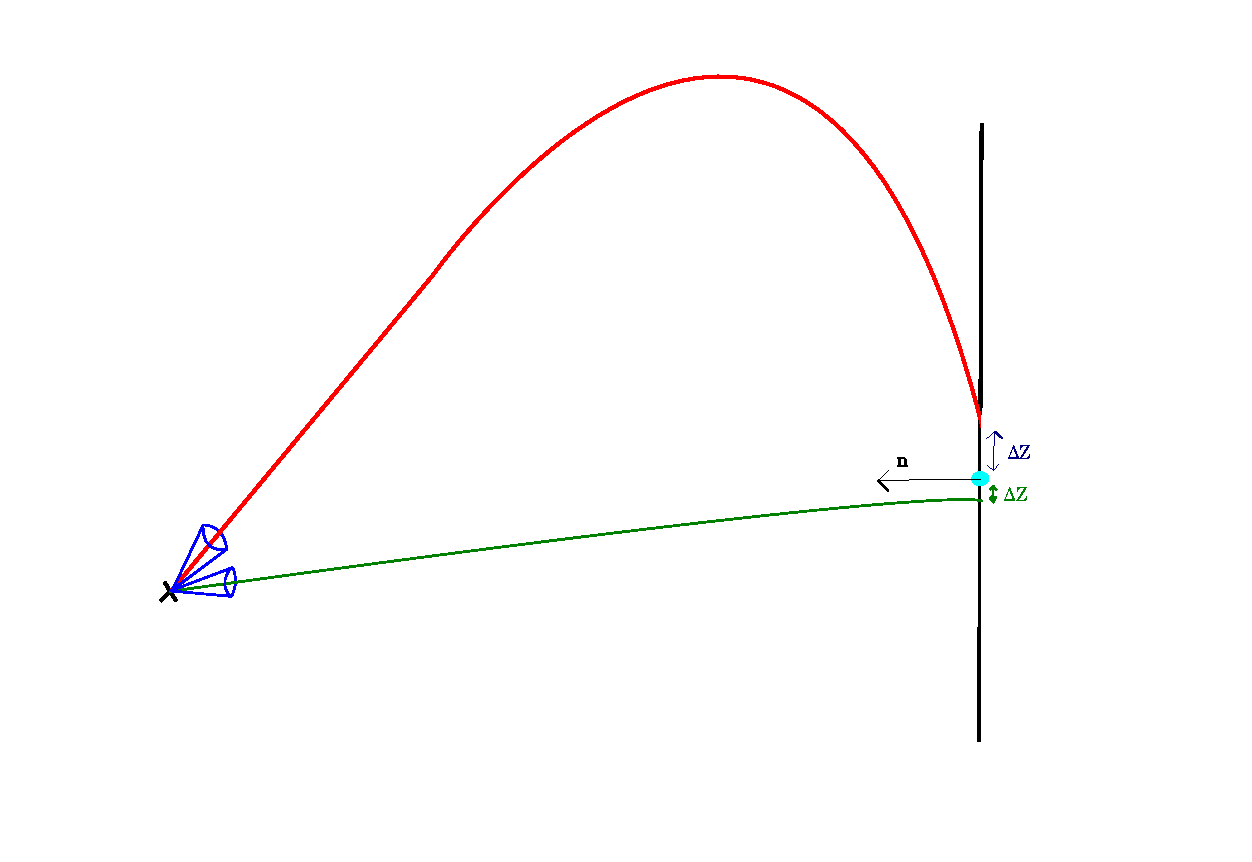
\includegraphics[width=0.7\textwidth]{PrincipleHybridIllu.pdf}
  \caption{The scipy algorithm shoots rays in a direction within the blue cone angle intervals and minimizes the $\Delta z$ that gets returned}
  \label{fig:PrincipleHybridIllu}
\end{figure}
The function we'll minimize is then delta\_z\_squared which just squares the
value which delta\_z returns as we want to do away with negative values (so we
can minimize to $\Delta z=0$). We use the previously found angle boundaries as
the boundaries for this minimization algorithm, meaning that if the 2 zenith
angle intervals $[\theta_1,\theta_2]$ and $[\theta_3,\theta_4]$ were found in
the first step of the algorithm it will first minimize $\Delta z^2$ within the
first angle interval and find it's solution and then within the second angle
interval. With this our algorithm is done, it does have a fail-safe as well in case
that the first step, finding the launch regions, doesn't find the 2 launch
regions.  Namely it reverts back to being the iterative ray tracer.

\section{Performance Optimization} 
We wish to optimize this algorithm to make
it as fast as possible.  To consistently test the algorithm after every
particular change in a parameter we'll be randomly generating vertex
interaction positions, keeping the detector at the fixed location of (0,0,-100).  To
this end the numpy random module was used to generate random coordinates, the
considered square (as there is only a z component to the ice model, the 3D
problem has cylindrical symmetry and thus essentially only a 2D problem) is
x:0.1km,4km and z:-0.1km,-3km\footnote{This start at 100m depth was to get
around issues concerning events that won't even trigger in a full simulation}.
Every simulated point shown in the following subsections consists of at least
500 random initial positions.  As the speed of the algorithm is computer
dependent the algorithm's speed is always plotted relative to the iterative ray
tracer's speed, simulated with the same coordinates and under equal computer load.

Now we don't want to just achieve higher speed in our algorithm, we also want
to at least have the same accuracy as the iterative ray tracer, if not even better.
To this end we need to check with an "exact solution". There is only one candidate
that fits this role: \textit{the analytic ray tracer}. The plan is thus to use the
exponential ice model as a testing ground for the hybrid ray tracer and solving each
vertex-detector ray tracing problem with both the iterative, analytic and hybrid ray tracer.
After having solved for the \textbf{propagation time} (meaning the time it takes the ray to
propagate from the source to the detector) and the \textbf{arrival zenith angle} (the zenith angle
the ray makes at the detector) for each of the algorithms we can infer the accuracy of a particular
algorithm by how much it differs from the solution found through the analytic ray tracer.
\subsection{Length of the normal vector}
\begin{figure}
	\centering
	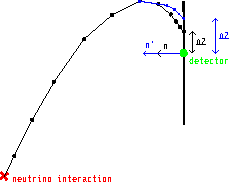
\includegraphics[width=0.6\textwidth]{figures/PrincipleNormIllu.pdf}
	\caption{the steps taken are illustrated with the dots, the spacing reduces close to the detector. changing
	the normal vector changes the spacing and thus the accuracy.}
	\label{fig:normexpl}
\end{figure}
Whilst figuring out what was wrong with the initial \textit{minimizer} we
stumbled on the fact that radiopropa has a little weird quirk.  As visually
explained in figure \ref{fig:normexpl}, the size of the normal vector seems to
influence how big radiopropa's ray tracer's step size is taken close to the
detector.  This thus influences the accuracy and total computational time
taken. The results of varying the length of this normal vector, comparing the
accuracy (in timing and arrival zenith) with the analytic ray tracer and the computational time with the
iterative ray tracer, are shown in figure \ref{fig:norminfl}.  
Looking at these figures we can make, what would
normally be rather obvious but is interesting nonetheless, a first optimization
conclusion: take the normal vector length to be 1 unit in radiopropa.
We can conclude this as the calculation speed seems to be minimal there 
and the accuracy dropping rapidly after 1 meter.
Note that none of the measurements performed during this chapter have
error flags, this is because this optimization procedure is only to get
us roughly into the right ballpark.

\begin{figure}
	\centering
	\begin{minipage}{\textwidth}
		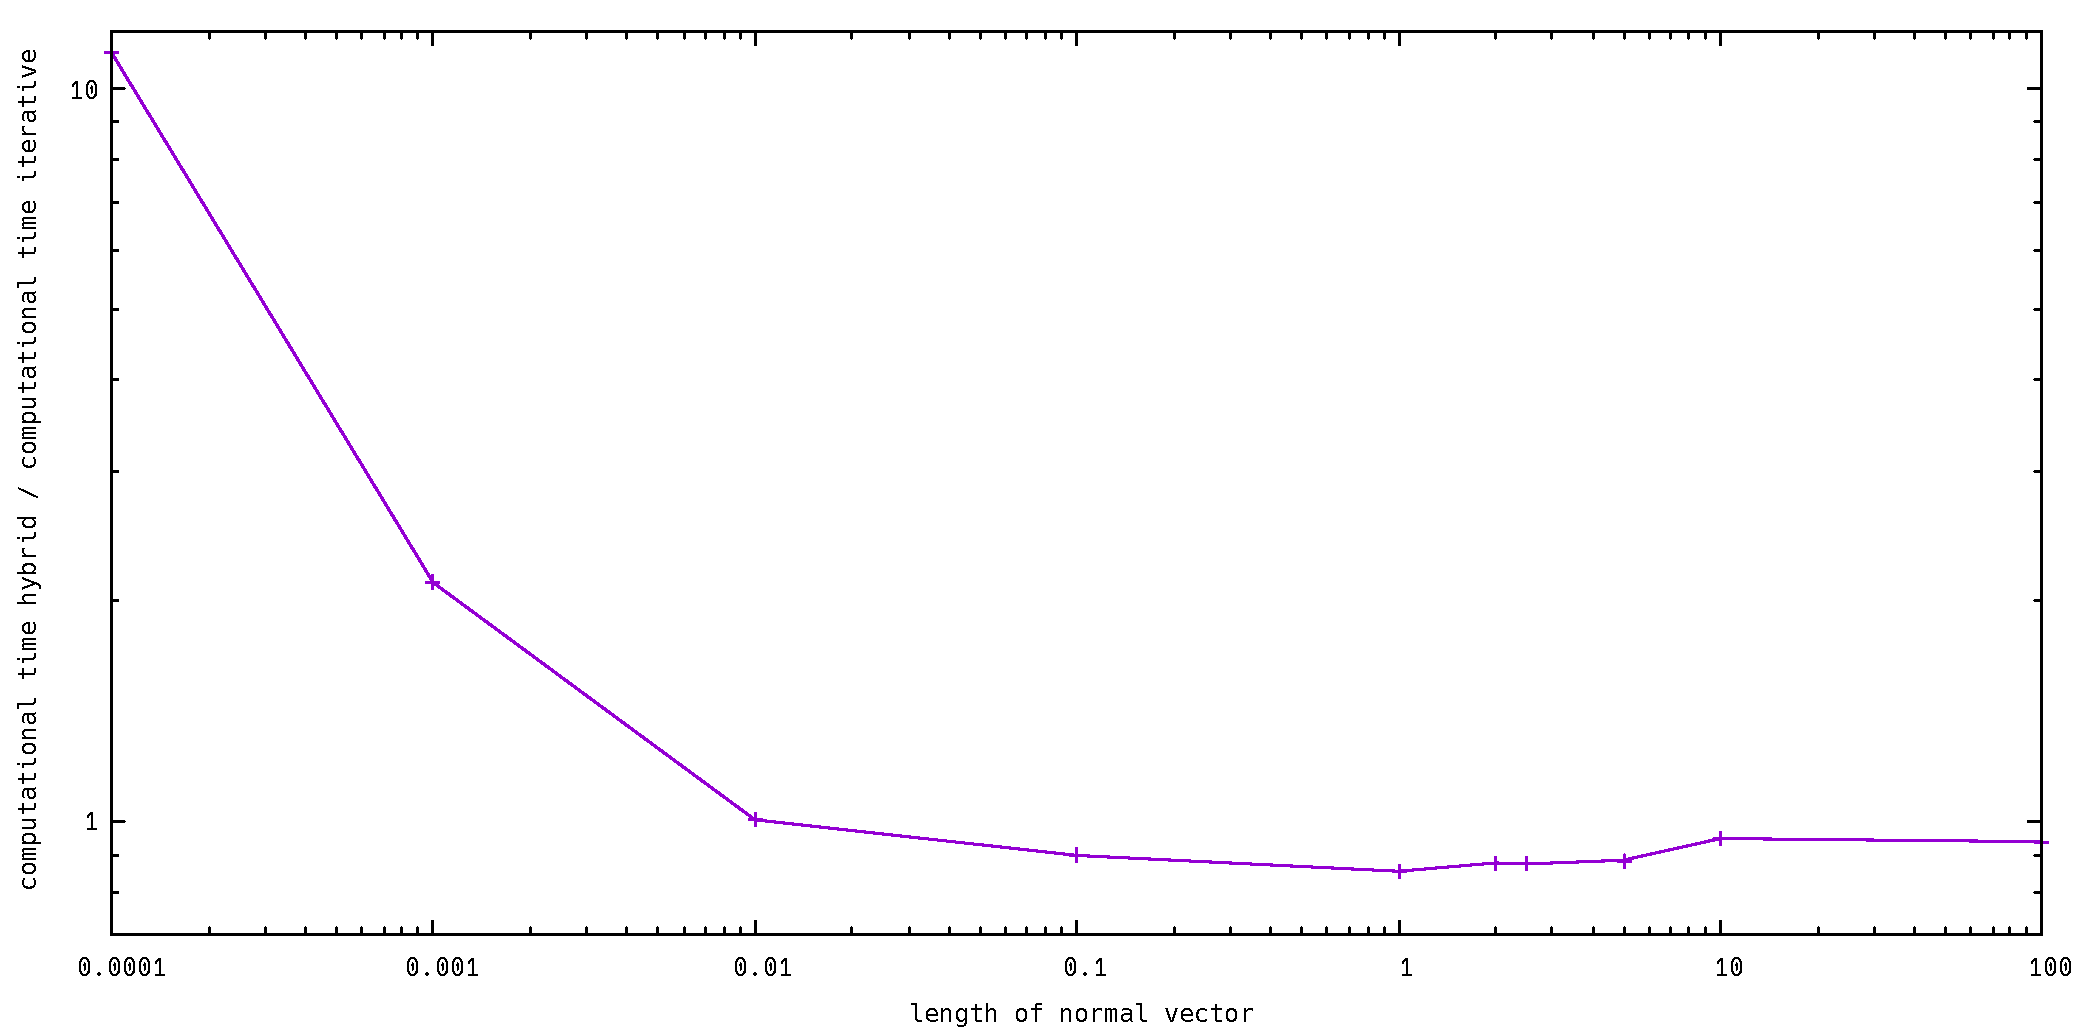
\includegraphics[width=0.9\textwidth]{figures/NormVsTime.pdf}
	\end{minipage}
	\begin{minipage}{\textwidth}
		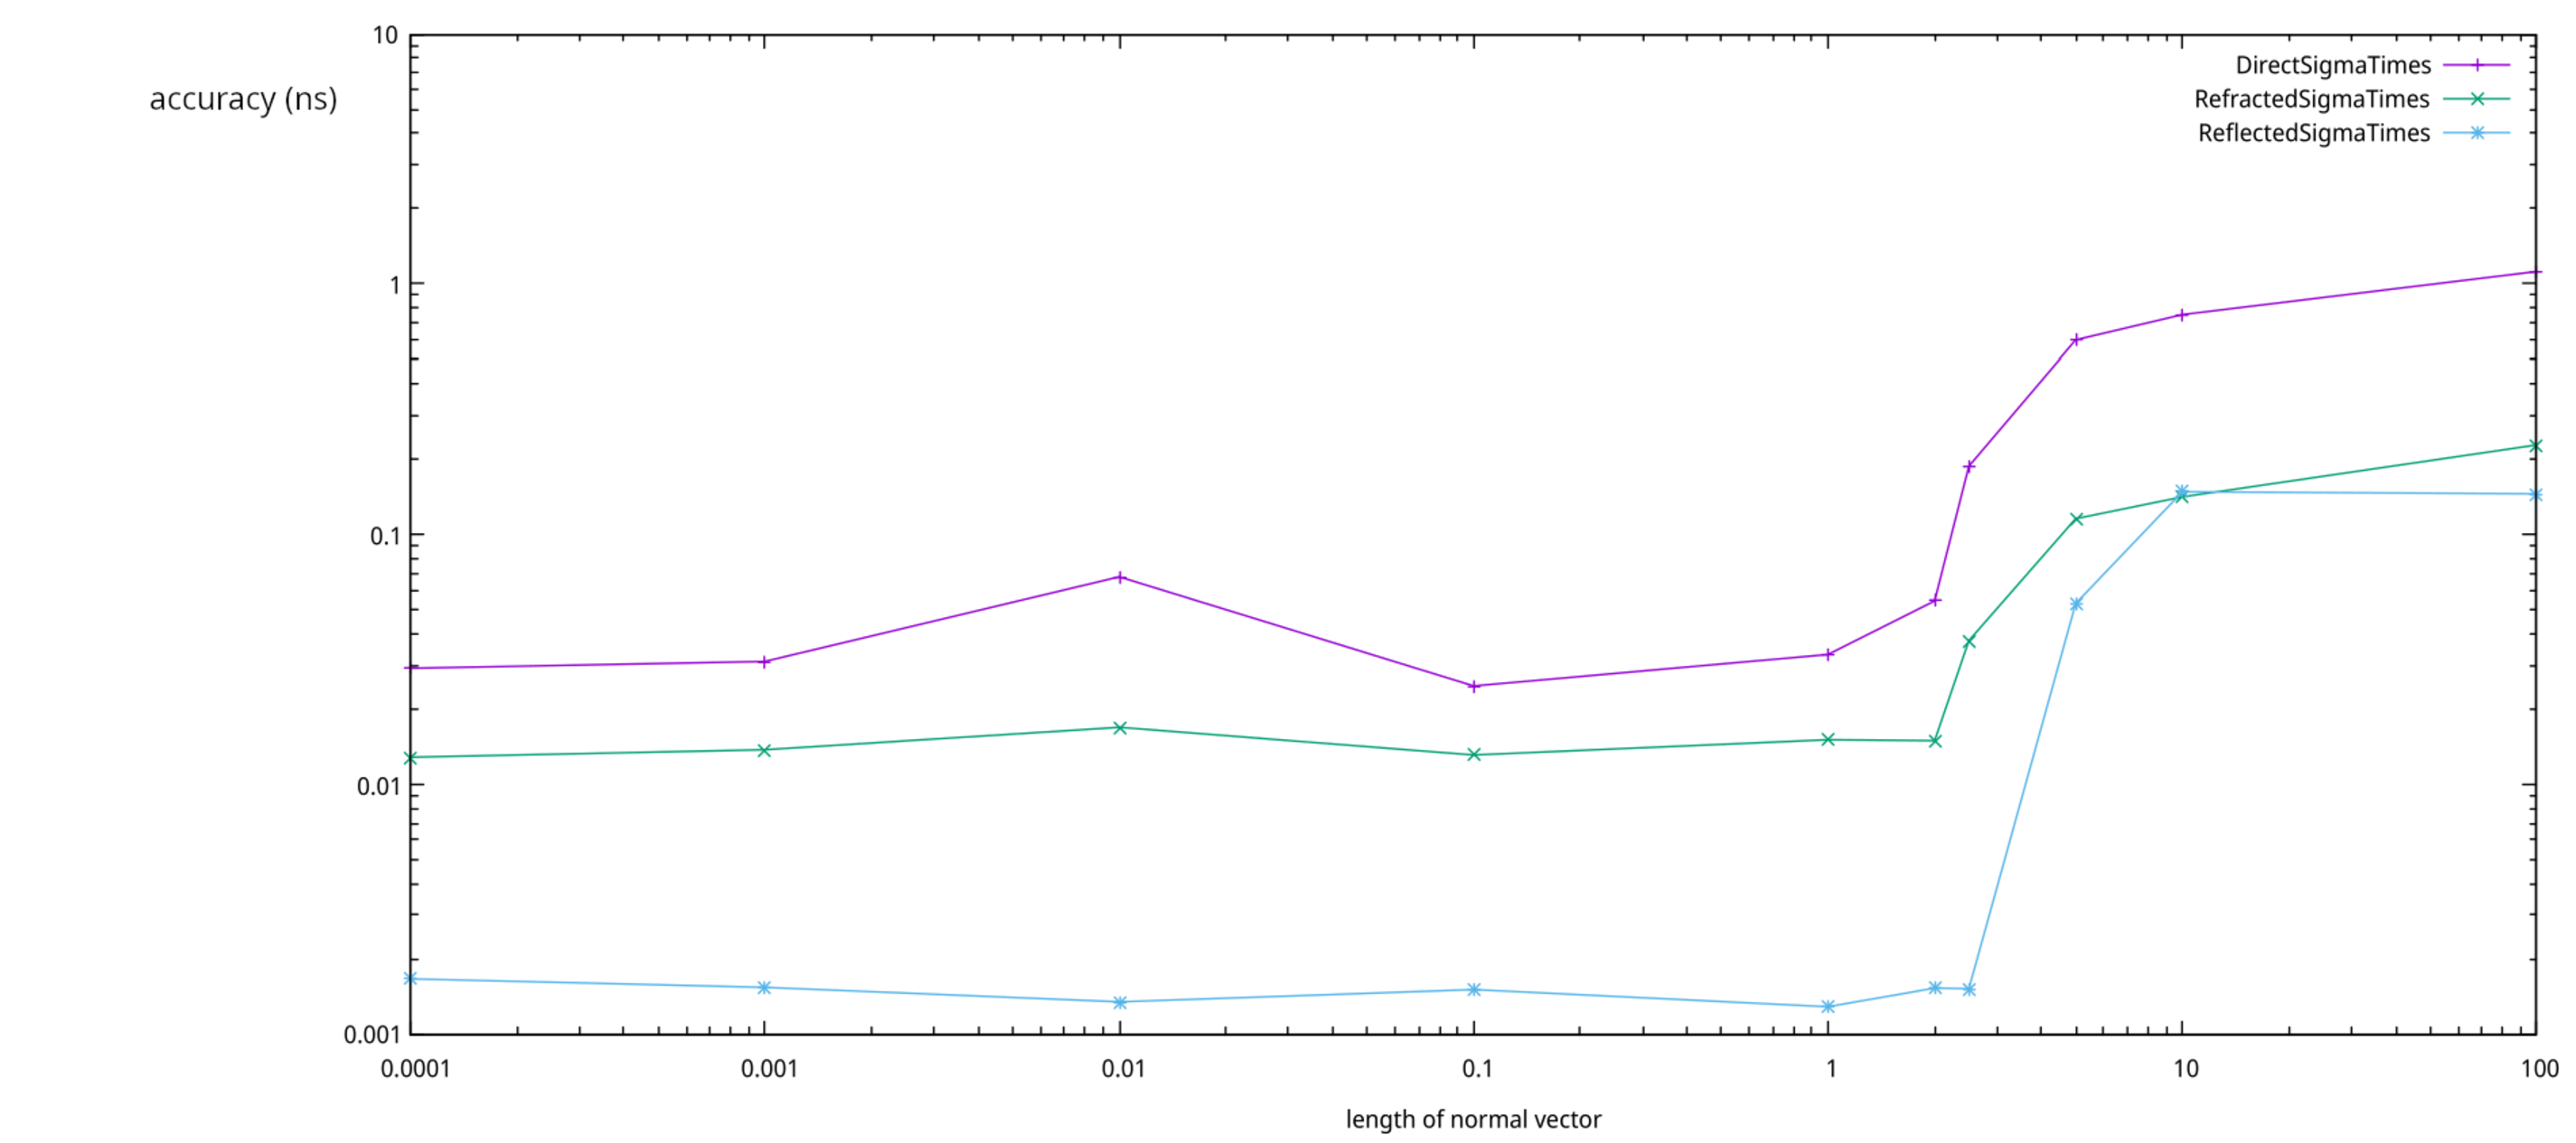
\includegraphics[width=0.9\textwidth]{figures/NormVsSigmaTime.pdf}
	\end{minipage}
	\begin{minipage}{\textwidth}
		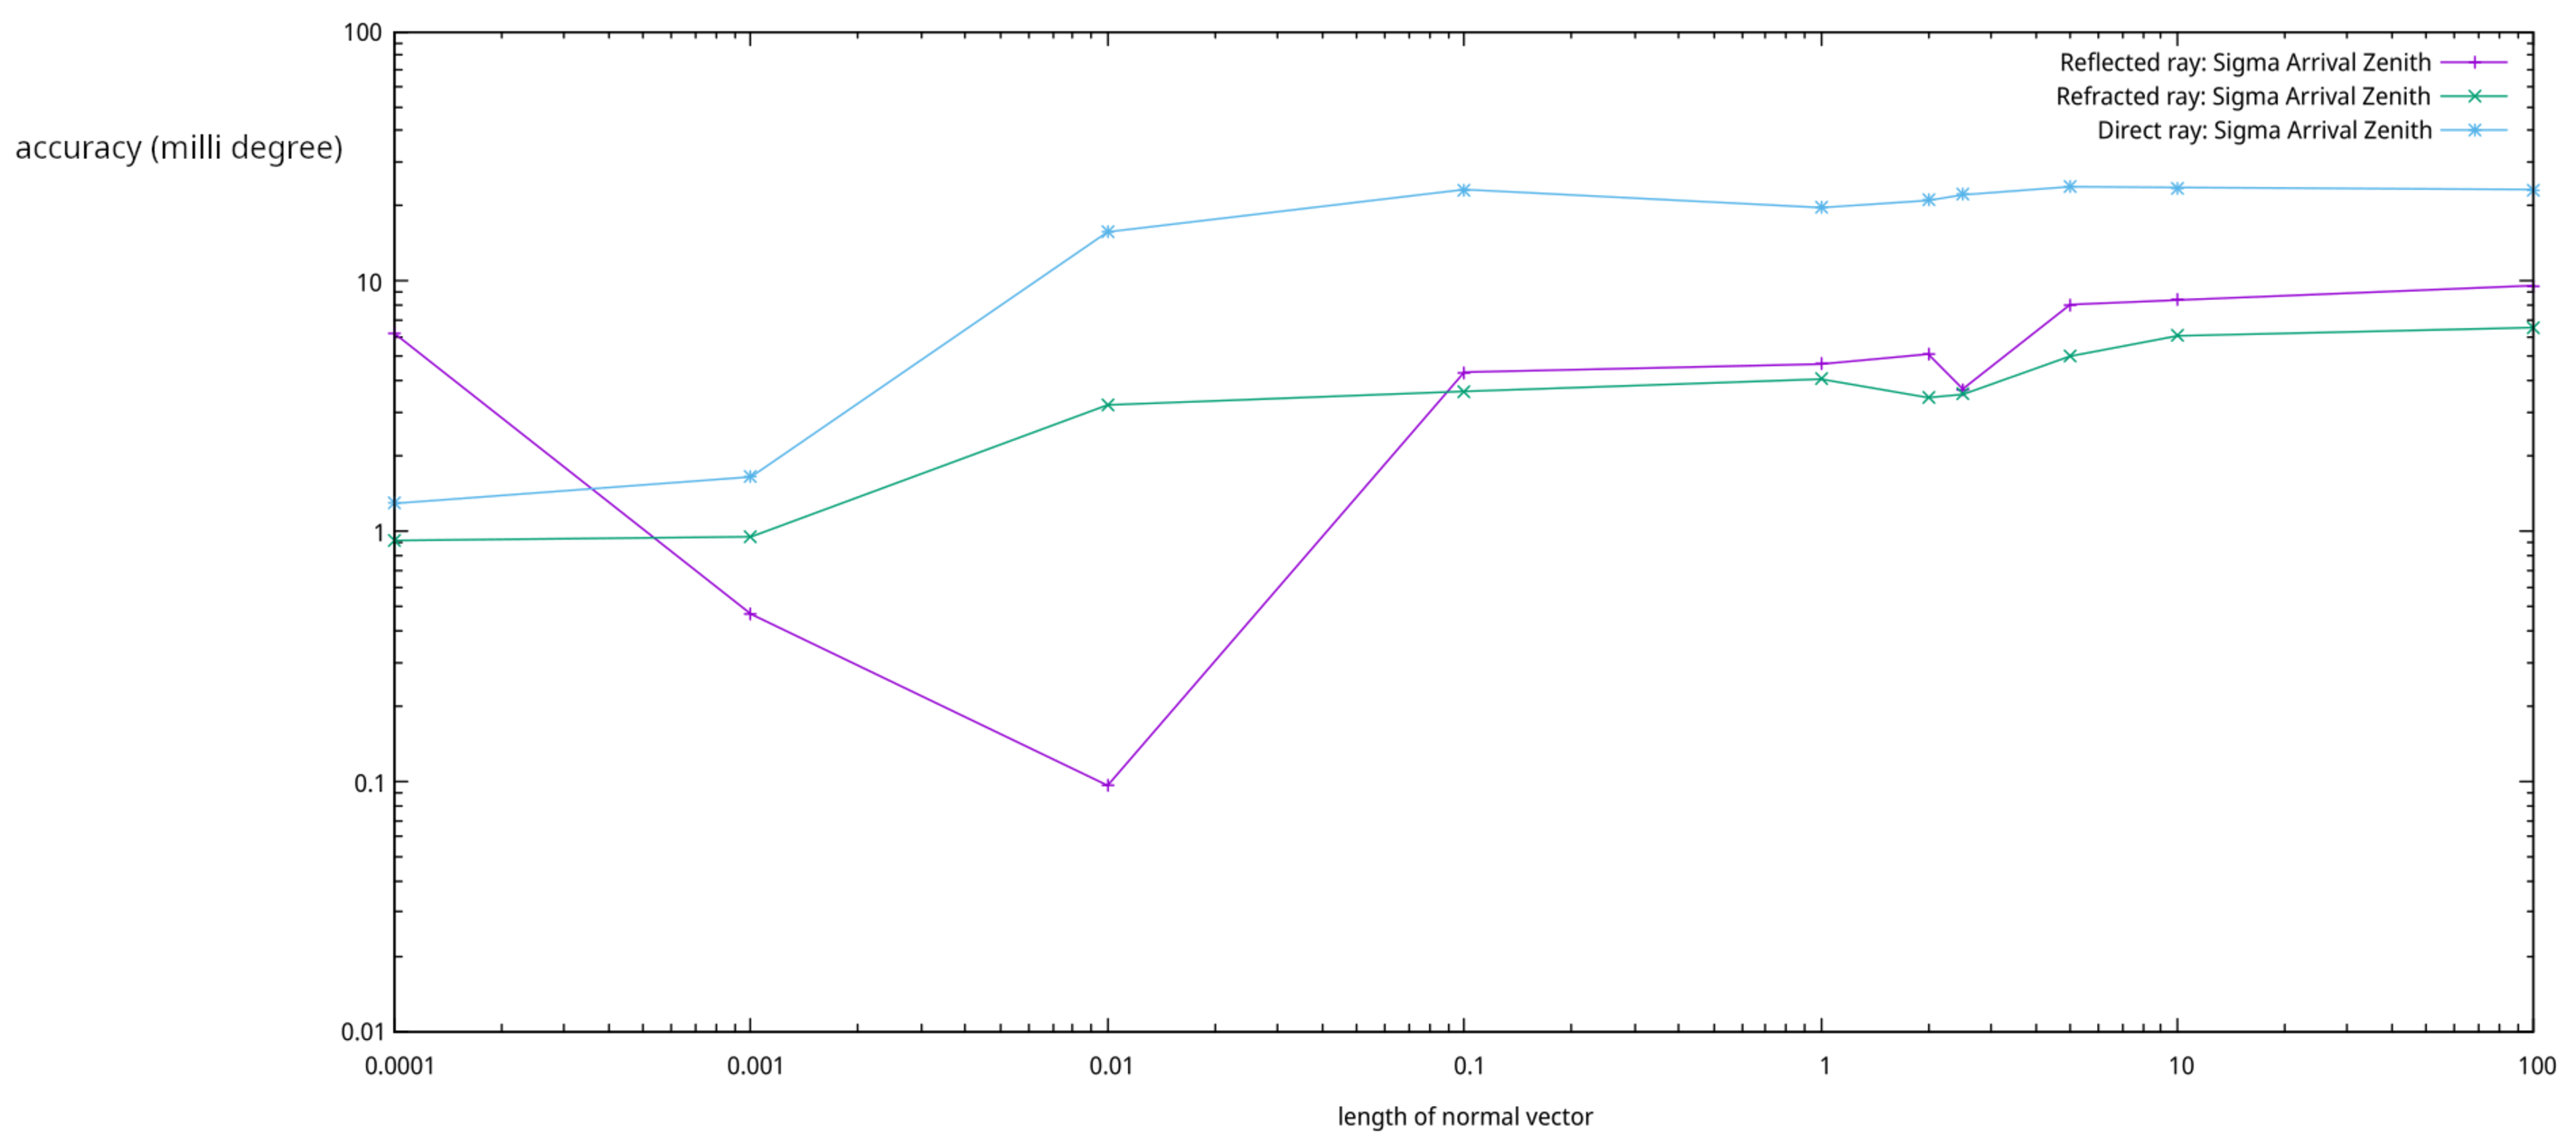
\includegraphics[width=0.9\textwidth]{figures/NormVsSigmaAZ.pdf}
	\end{minipage}
\caption{The speed first lowers with larger normal vector lenght, reaching a minimum near 1 but the accuracy on timing gets worse after a length of 1. We thus
conclude to take a normal vector length of 1.}
\label{fig:norminfl}
\end{figure}

\subsection{ztol}
We'll now change the \textit{tolerance}, with this we mean when 
the minimization algorithm returns a $\Delta z$ smaller than a certain
threshold "ztol" the ray will be accepted as the solution.  
The results from analogous comparisons as
previously discussed are shown in figure \ref{fig:ztolinfl}.
\begin{figure}
	\centering
	\begin{minipage}{\textwidth}
		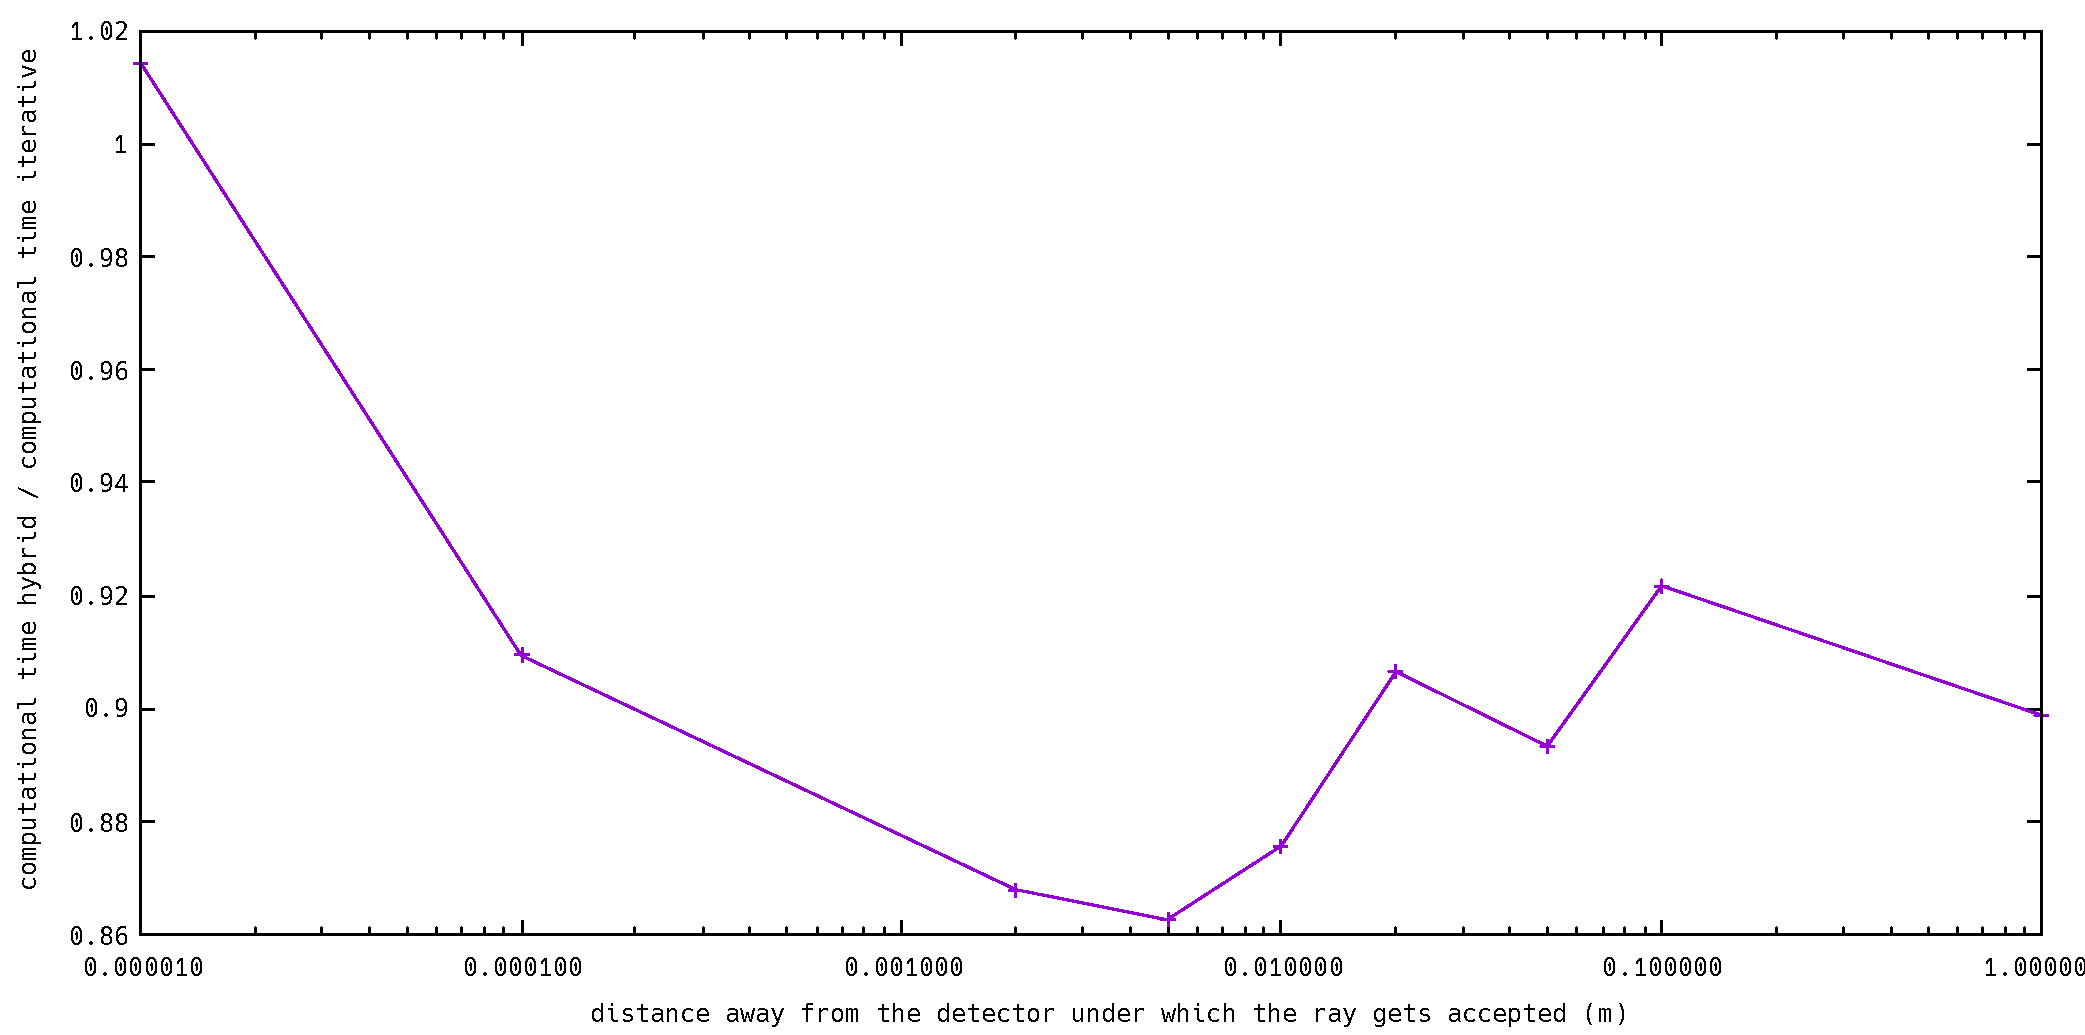
\includegraphics[width=0.9\textwidth]{figures/ZtolVsTime2.pdf}
	\end{minipage}
	\begin{minipage}{\textwidth}
		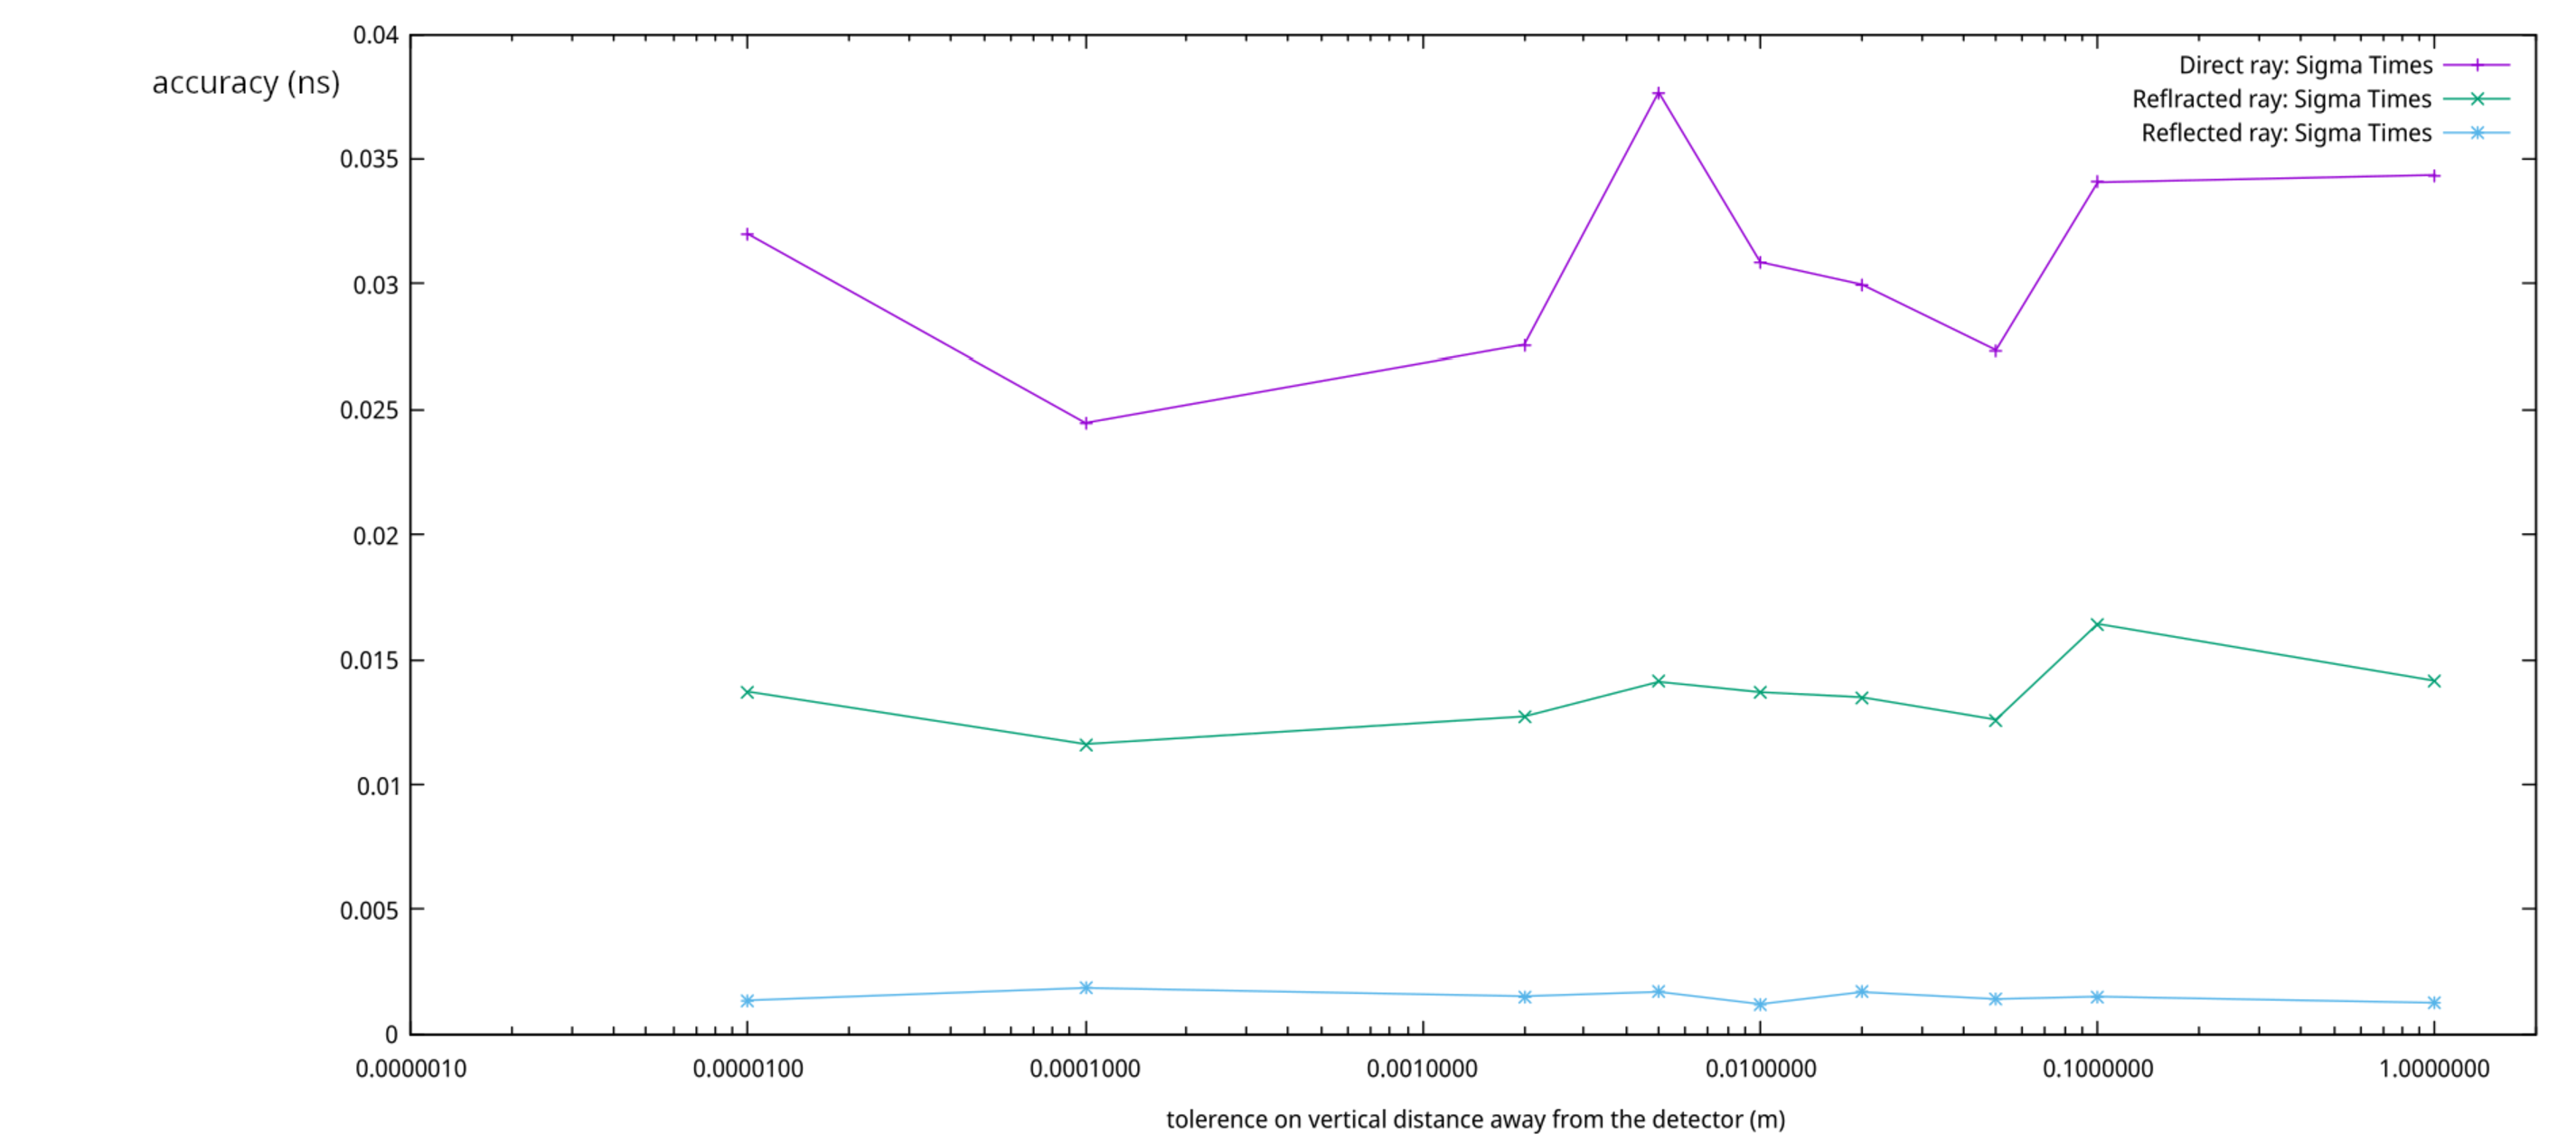
\includegraphics[width=0.9\textwidth]{figures/ZtolVsSigmaTime.pdf}
	\end{minipage}
	\begin{minipage}{\textwidth}
		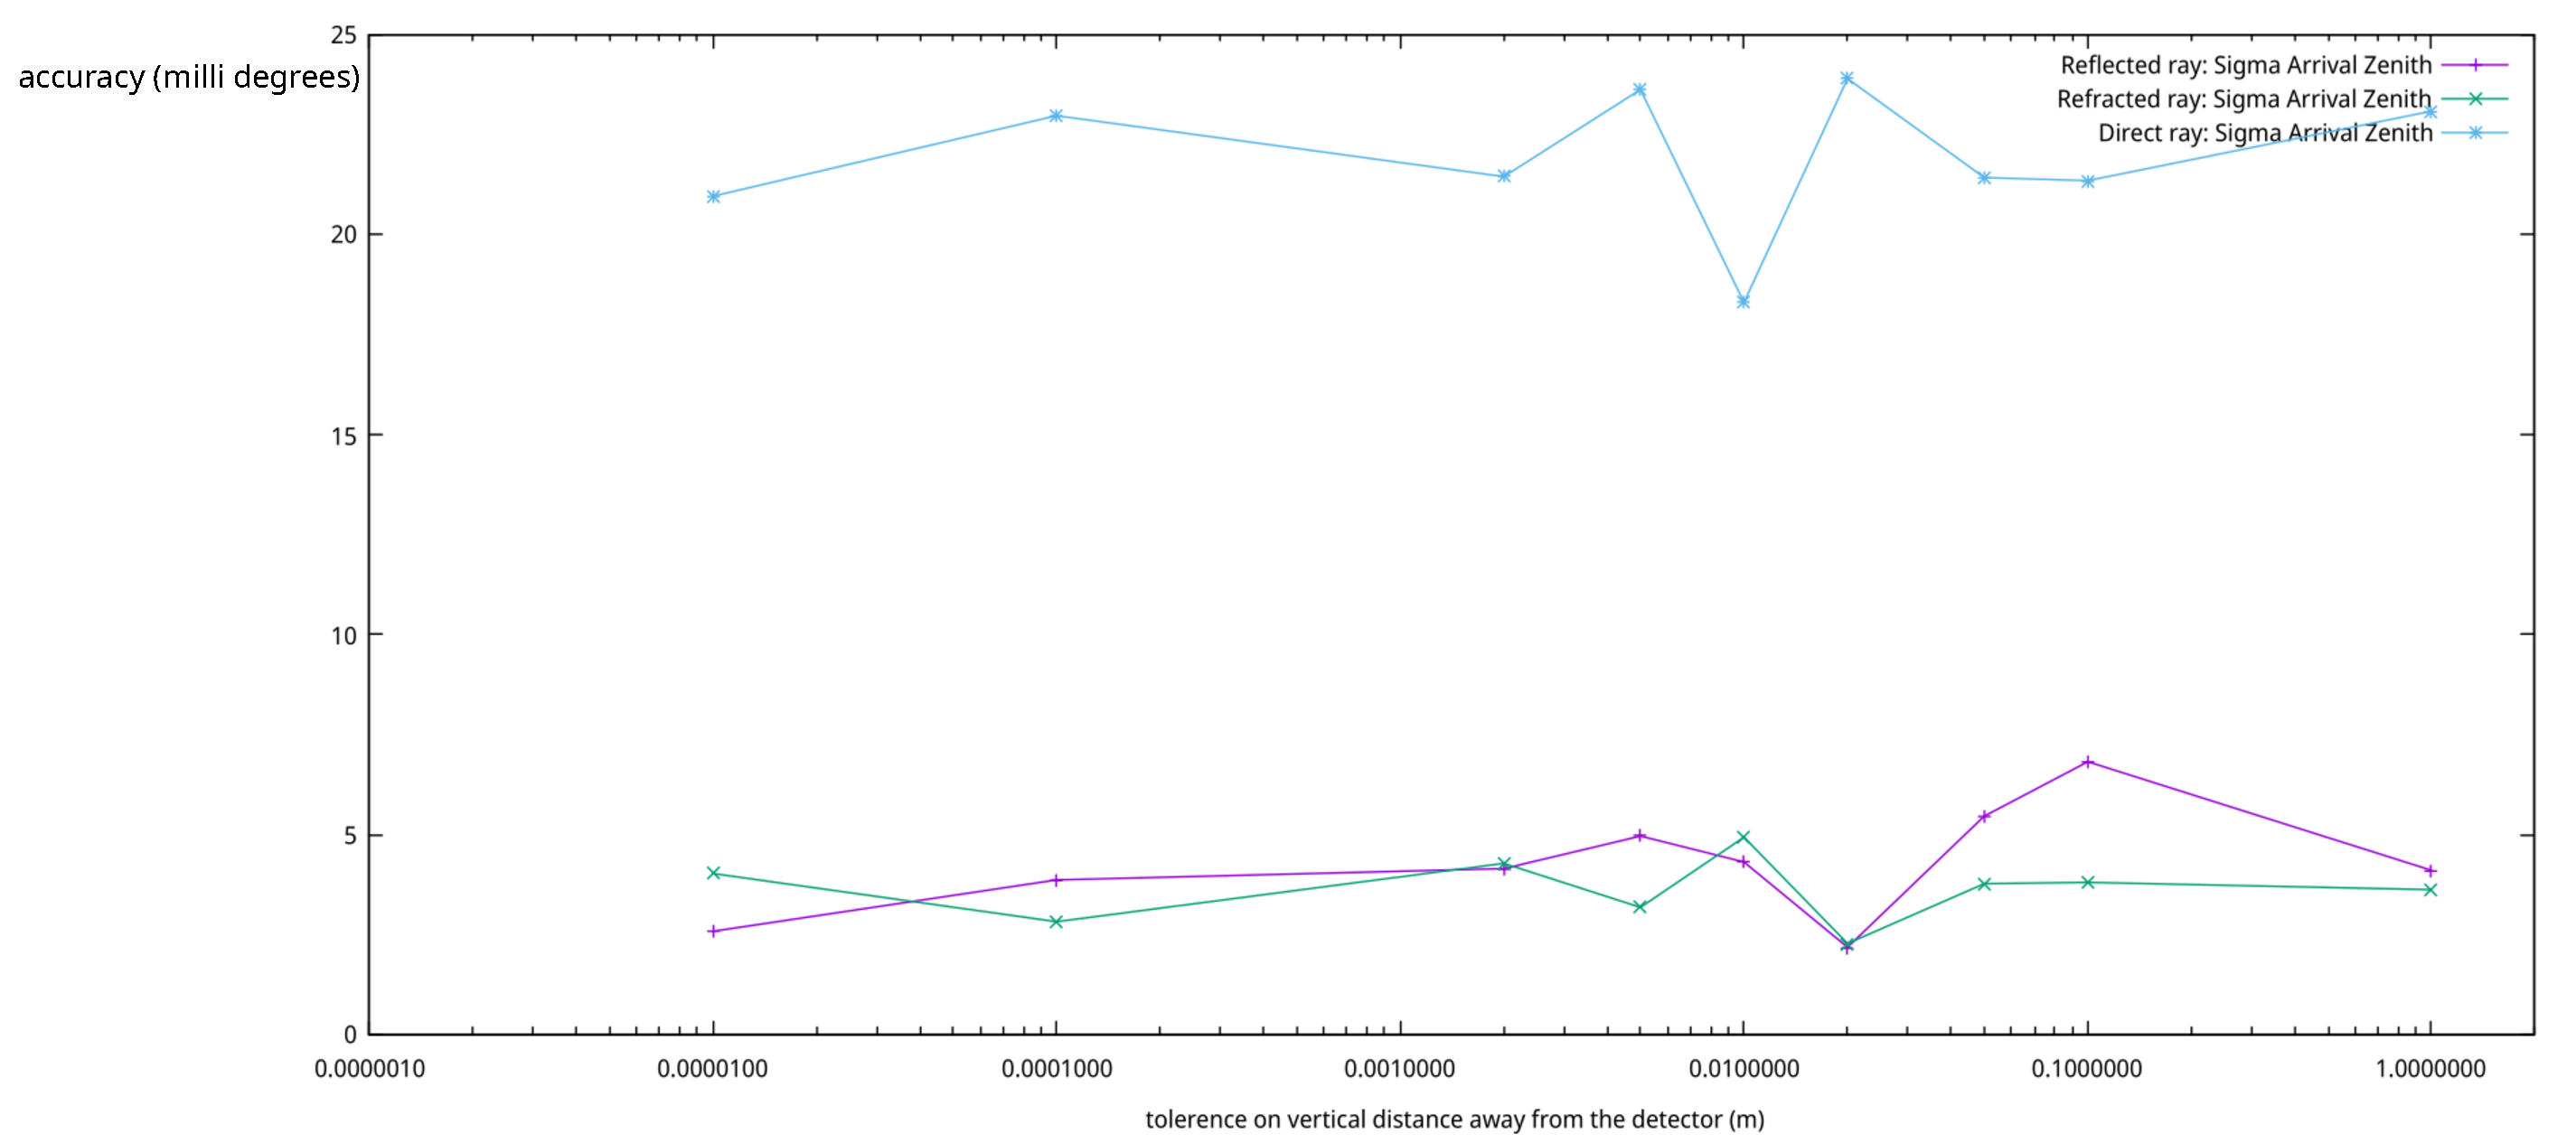
\includegraphics[width=0.9\textwidth]{figures/ZtolVsSigmaAZ.pdf}
	\end{minipage}
\caption{the solution seems to reach a minimal time at a tolerance of 5cm whilst both the accuracy on timing and the one on the zenith angle stay roughly the same, we thus conclude the zenith
tolerance to be 0.05m for optimal computing.}
\label{fig:ztolinfl}
\end{figure}
\newpage
There seems to be a minimum around 0.05m, looking at the
accuracy for this tolerance it seems sufficient to be used.  We can thus infer
the second optimization conclusion: take ztol to be 0.05 m.

\subsection{Sphere Size \& Step Size}
The initial rays are sent out in steps of a certain angle and with a sphere
around the detector of a certain size. Varying the parameters of this first
step of the algorithm (e.g the step size and sphere size) might thus have an
effect on both the accuracy and the computational time.  As this initial search
for launch angle regions is also the slowest step in the hybrid ray tracer (takes
$\approx 57\%$ of the total computation time)
it's also the most important step to optimize. The optimization procedure is as
follows: change the sphere size and loop over various step sizes, recording the
speed. Note that, as we have to vary 2 parameters, we can't really look at
accuracy here. This isn't needed however as we'll see that after finding the
optimal solution the accuracy is still sufficient, apart from one part where it is
needed: when insufficient solutions are found. 

As we wish this algorithm to be better than the iterative ray tracer, it'll need to
at least find as many solutions as the iterative ray tracer does.  If, for a
particular random interaction vertex location, less solutions are found by the
hybrid ray tracer than for the iterative ray tracer, this parameter choice will
be thrown away (and colored differently).  The results are shown in figure
\ref{fig:SphereStepInfl}, the points colored red are unusable following the previously
discussed criterium of sufficient solutions.

The lower on the graph the points lie, the better. If we combine all the green points into a single plot
we get what is shown on figure \ref{fig:SphereStepFinal},
looking at the lowest point, we see that an optimal sphere size seems to be at 45m accompanied
by a step size of 0.7°, this is in contrast to the iterative ray tracer where a sphere size of 25m and stepsize
of 0.5° is used. Note that changing these values for the iterative ray tracer doesn't change it's speed nor accuracy.

The programs used in making these plots can be found \href{https://github.com/arthuradriaens-code/projects-mt}{here}
under the folder "testhybrid".
\begin{figure}
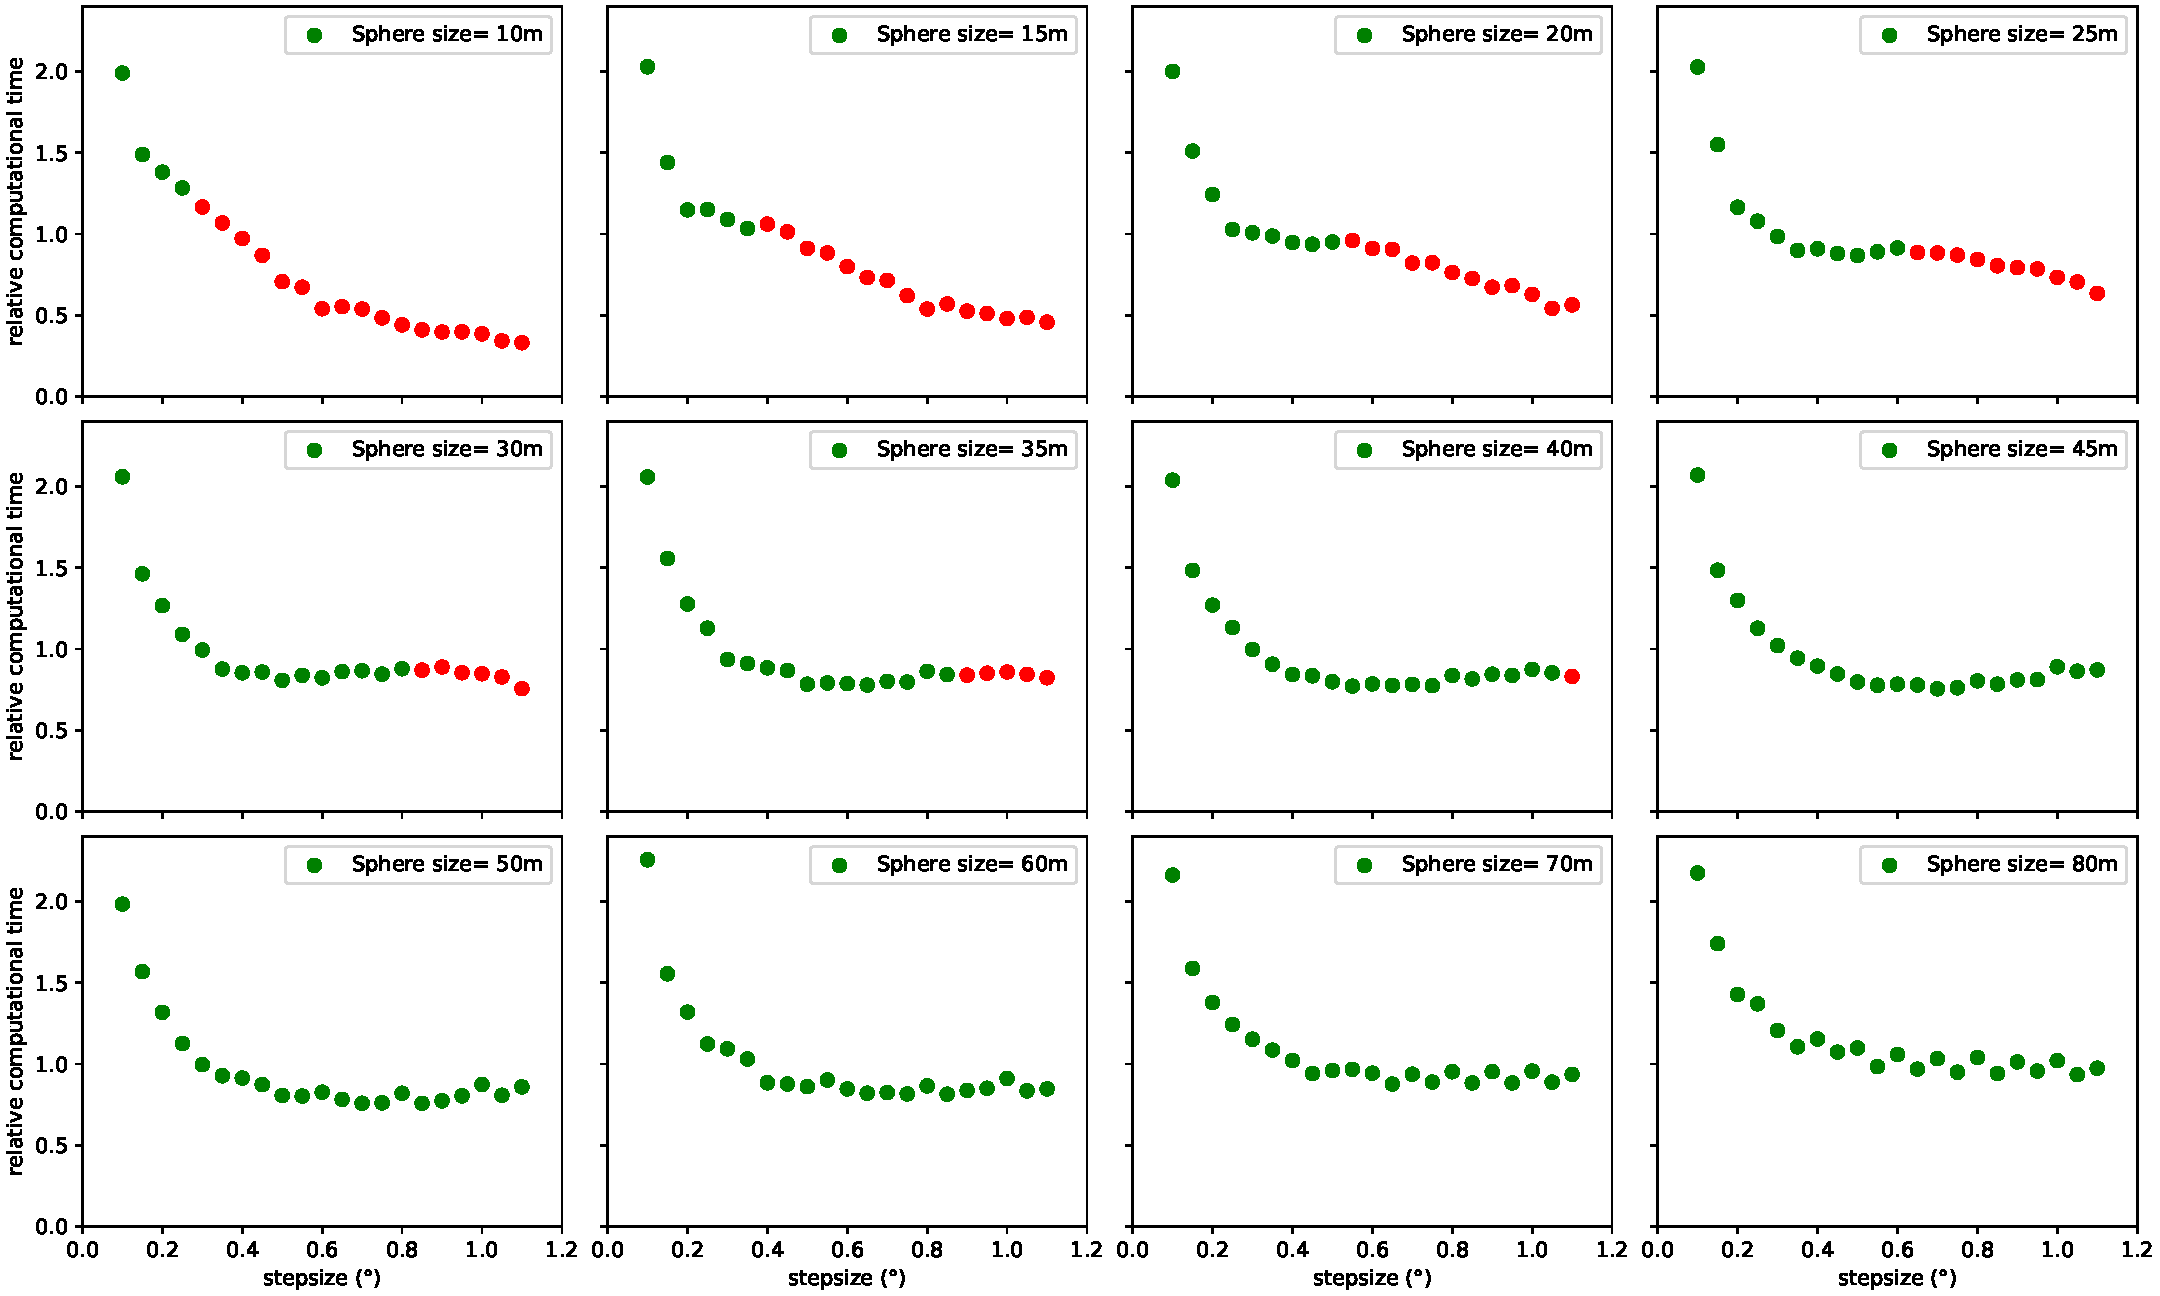
\includegraphics[width=\textwidth]{figures/subplotofallstepsphere.pdf}
\caption{The data in green is acceptable, at high sphere size the geometric effects start to play a role and staggering is observed}
\label{fig:SphereStepInfl}
\end{figure}
\begin{figure}
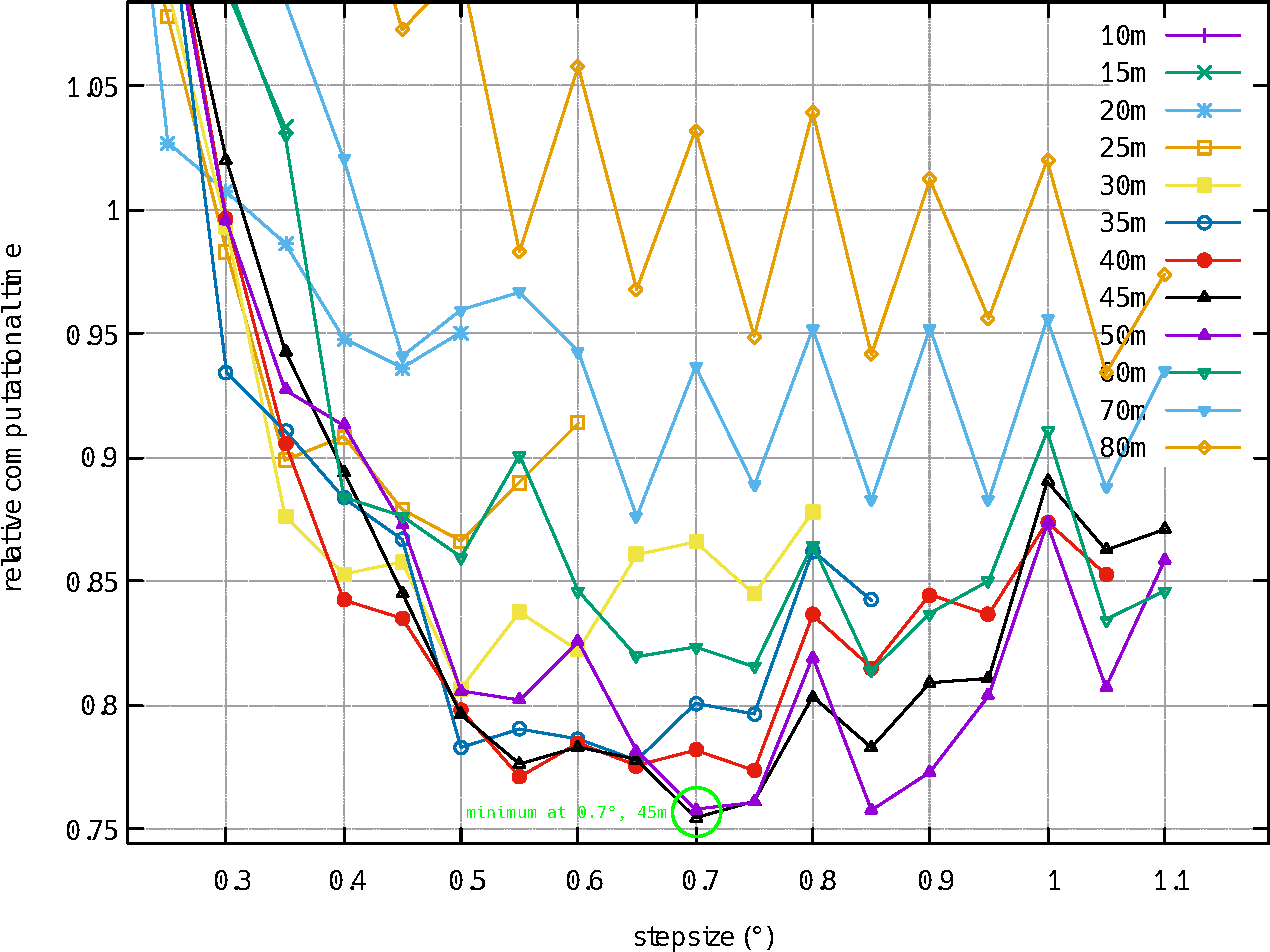
\includegraphics[width=\textwidth]{figures/SphereAndStepFinalWithMark.pdf}
\caption{Green values in variation in sphere and angle step size, the lower the better. Max speed (lowest point on the figure) at 0.7° as step size and 45m sphere size}
	\label{fig:SphereStepFinal}
\end{figure}
\newpage
\subsection{Conclusion of optimization}
How does the hybrid ray tracer perform relative to the iterative ray tracer if we use 
the previously optimized variables? After doing a simulation of 1000 random source locations (double the previous amount) with
the iterative, analytic and hybrid ray tracer and comparing both the iterative to the analytic and the hybrid to the analytic
we get what's shown in figures \ref{fig:acchyb} and \ref{fig:accit}. Where we can clearly see that the hybrid
ray tracer is more accurate, now during this simulation we also recorded the computational speed, the fractional
speeds relative to the analytic ray tracer are presented below:
\begin{itemize}
	\item iterative: $5.93 \times 10^{-5}$ computations/analytic computation
	\item hybrid: $7.97 \times 10^{-5}$ computations/analytic computation
\end{itemize}
The hybrid ray tracer is thus 33.7\% faster than the iterative ray
tracer. The speed difference with the analytic ray tracer might seem
quite overwhelming but this can get mitigated in the future if part
of the hybrid ray tracer gets re-written in a compiled language
like C++ in which the analytic ray tracer was written.

\begin{figure*}
	\centering
\begin{minipage}{0.49\textwidth}
	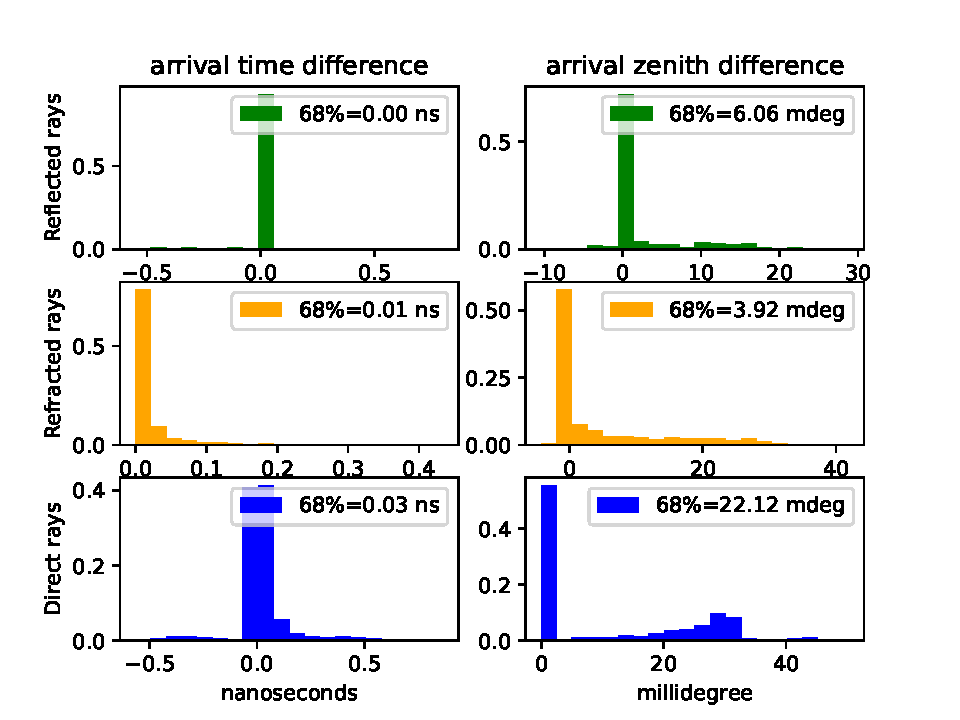
\includegraphics[width=1.1\textwidth]{figures/hybrid_comparison_N_1000.pdf}
	\caption{Hybrid}
	\label{fig:acchyb}
\end{minipage}
\begin{minipage}{0.49\textwidth}
	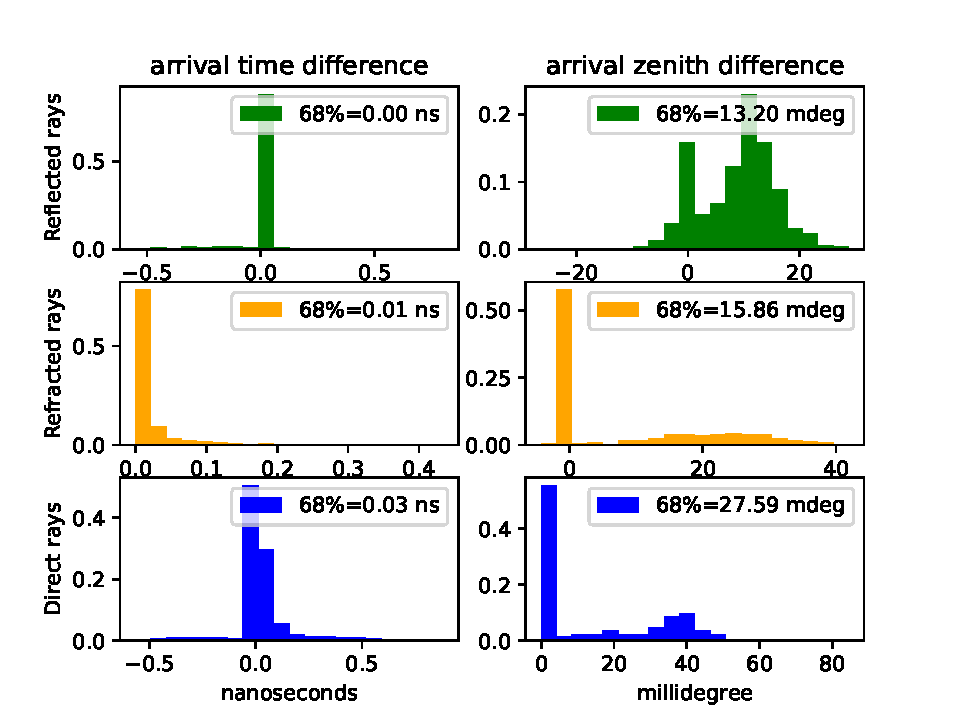
\includegraphics[width=1.1\textwidth]{figures/iterative_comparison_N_1000.pdf}
	\caption{Iterative}
	\label{fig:accit}
\end{minipage}
\end{figure*}



\chapter{Weather Balloon}
\label{chap:WB}
In this chapter we'll infer optical information about the ice the detectors reside in
using radio signals coming from a weather balloon flying over the stations. 

Every day in the summer, 2 times a day, a weather balloon gets launched
from base camp at Summit in Greenland. This weather balloon has an antenna
strapped to it constantly emitting a sinusoidal signal of 0.403GHz.

We can use this signal to find the index of refraction locally at the phased
array.  We'll go about this by first finding the difference in timing between the
channels by fitting the balloon's sinusoidal signal to the data, and then doing
a plane wave reconstruction using the angle the balloon makes with the channel.
With this plane wave reconstruction we can then find the index of refraction locally at the channel.  This procedure will
be explained more in depth over the following sections.

Prior to the measurements we'll need to be able to predict how accurate our
findings will be, for this we'll need to run a simulation with the hybrid ray
tracer (explained in chapter \ref{chapter:hybrid}).  
There is one change that needs to happen to our algorithm in order
to be able to simulate this: The air observer has to be removed to make
ray tracing possible from within the air into the ice and onto the detector\cite{hybrid}.

\section{Plane Wave Reconstruction}
We want to do a plane wave reconstruction of the balloon's position as this
will enable us to infer the index of refraction between chosen channels.
Example paths the weather balloon produces that end up in the deep channels are
shown in figure \ref{fig:Example trajectory}, here the balloon emits a signal
which propagates straight in the air and then refracts in the ice. Locally in
the ice we can assume the wave to come in as a plane wave.
\begin{figure}
	\centering
	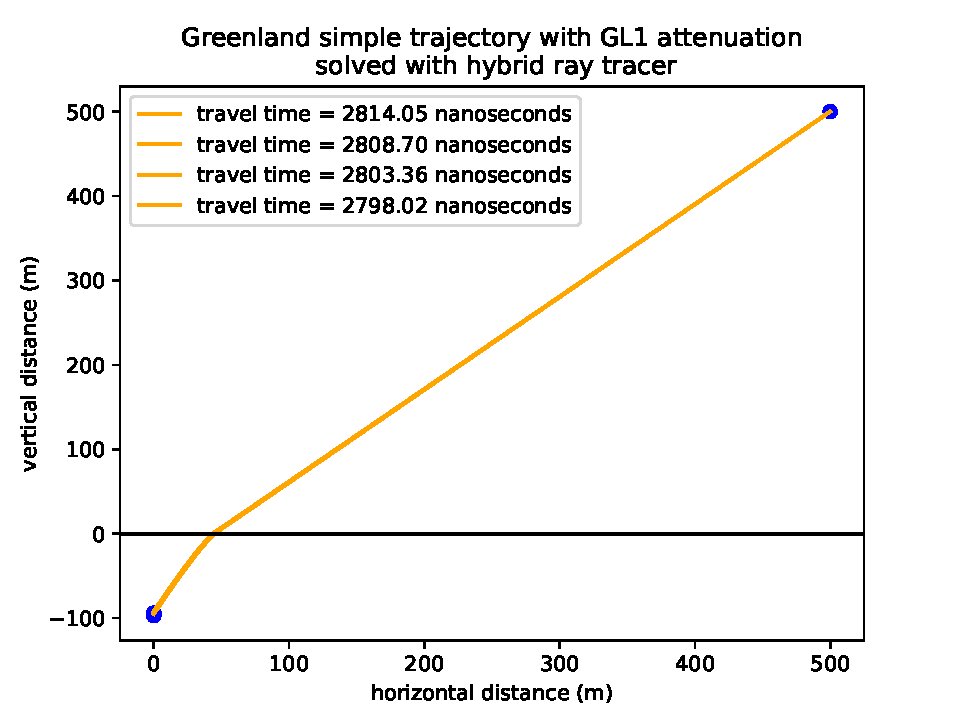
\includegraphics[width=0.7\textwidth]{weerballontraject.pdf}
	\caption{Example trajectory of rays coming from a weather balloon (red top right dot) and going through the ice to the various detectors (blue dots bottom left)}
	\label{fig:Example trajectory}
\end{figure}
\begin{figure}
	\centering
	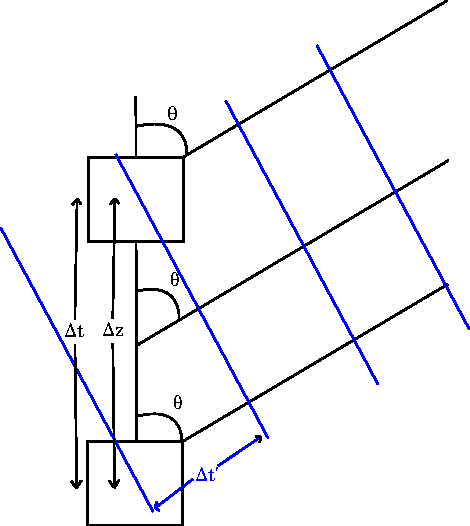
\includegraphics[width=0.7\textwidth]{planewave.pdf}
	\caption{The incoming signal can locally be seen as a plane wave, here drawn in blue. The channels are drawn in gray but are assumed to be points located at the center.}	
	\label{fig:Plane Wave}
\end{figure}

The arriving plane wave is shown as parallel lines in blue on figure \ref{fig:Plane Wave}. The
plane wave reconstruction method can be understood by taking a closer look at this figure, 
the radio waves coming from the weather balloon make a certain zenith angle $\theta$ with the detectors. The top detector (top box)
detects the wave at a certain time $t_1$, the bottom detector detects it at a
time $t_2$. After deciphering the data RNO-G recorded we'd thus see that these
two detectors got a signal $\Delta t = t_1 - t_2$ seconds apart from each other.
Now ideally this observed time is equal to the time it would theoretically take a plane
wave to propagate that distance ($\Delta t'$) which we can calculate from the geometry of
the problem and dimensional analysis:
\begin{equation}
	\Delta t' = \frac{m}{(m/s)} = (s/m)*m = v^{-1} * m = v^{-1} \cos\theta \Delta z
	\label{eqn:deltataccent}
\end{equation}
With $v = c/n$ the local speed of light, n the index of refraction at the depth in between
the considered channels and $\Delta z$ the distance between the channels. 
Thus if we know the zenith angle $\theta$, the difference in timing $\Delta t'$ and the distance between the channels $\Delta z$
we could infer the index of refraction at a certain depth as can be seen by reforming equation \ref{eqn:deltataccent}:
\begin{equation}
	n = \frac{\Delta t'}{\Delta z} \frac{c}{\cos\theta}
\end{equation}
We can actually roughly guess the angle, as for a balloon flying close to the
detector the incoming plane wave angle will be roughly the same as the angle the balloon
makes with the pair of channels ($\theta\approx\theta_b$).
At the actual index of refraction we thus expect the following function to show a 
minimum (go to zero):
\begin{equation}
	\eta(n) :=  (\Delta t - \Delta t'(\theta_b,n)) = \left(\Delta t
	- n\frac{\cos\theta_b \Delta z}{c}\right)
  	\label{eqn:eta}
\end{equation}
If we want to determine the index of refraction, 
we thus need to minimize equation \ref{eqn:eta}.

If we want to use more than 2 detectors at once however (which we'll
do for the phased array), we'll need to specify various functions to
minimize.  E.g if we have four detectors labeled 0 to 3 we'll have
to construct functions between detectors 0\&1, 0\&2, 0\&3, 1\&2,
1\&3 and 2\&3 . The further apart the detectors lie the larger the
function values and thus the more they will weigh in the sum. This importance to
further spaced channels is what we want as these will yield a more
accurate result. 
\subsection{simple plane wave reconstruction}
\label{seq:SimplePW}
To take into account all the different channels, we take the sum of the
various eta functions (as defined in equation \ref{eqn:eta}) and
thus minimize the following function with respect to the index:
\begin{equation}
	f(n) := \sum_{i=\text{channel pairs}}\eta_i(n) = \sum_{i=\text{channel pairs}}\left( \Delta t_i - \frac{n\cos\theta_b \Delta z_i}{c}\right) \equiv \sum_{i<j}\left( \Delta t_{ij} - \frac{n\cos\theta_b \Delta z_{ij}}{c}\right)
  	\label{eqn:PlaneWave}
\end{equation}
where $\Delta t_{ij}$ denotes the observed time difference between
channels i and j, similarly $\Delta z_{ij}$ denotes the distance
between channels i and j.
If this function $f$ gets minimized, the n leading up to this minimization
will be the answer we are seeking: the index of refraction between
the various detectors.  
We now want to find the error on the index we fitted this way. To find the error on our result we need an expression for the index, let's solve for n:
\begin{align}
	f(n) &= \sum_{i<j}\left( \Delta t_{ij} - \frac{n\cos\theta_b \Delta z_{ij}}{c}\right)\\
\sum_{i<j}\frac{n\cos\theta_b \Delta z_{ij}}{c}&=\sum_{i<j}\Delta t_{ij} - f(n)\\
	n &= \frac{c}{\cos\theta_b}\left(\frac{\sum_{i<j}\Delta t_{ij}}{\sum_{i<j} \Delta z_{ij}} - \frac{f(n)}{\sum_{i<j} \Delta z_{ij}}\right)
\end{align}
Let's assume an error on the difference in propagation time between channel i and j
($\Delta t_{ij}$) of $\delta t_{ij}$, which we'll find out later.  For the
positional accuracy we'll assume to know the detector location to within 1cm\footnote{this
is a reasonable estimate as this is the accuracy of the reported channel positions},
this will imply an accuracy on $\Delta z_{ij}$ of 2cm.

Let's now compute the error on our predicted index:
\begin{align}
  \delta n &= \frac{c}{\cos{\theta_b}}\delta\left(\frac{\sum_{i<j}\Delta t_{ij}}{\sum_{i<j} \Delta z_{ij}} - \frac{f(n)}{\sum_{i<j} \Delta z_{ij}}\right)\\
  \delta n &= \frac{c}{\cos{\theta_b}}\delta\left(\frac{\sum_{i<j}\Delta t_{ij}}{\sum_{i<j} \Delta z_{ij}}\right)+ f(n)\frac{c}{\cos{\theta_b}}\delta\left(\frac{1}{\sum_{i<j} \Delta z_{ij}}\right)\\
\end{align}
Note here the function $\delta$ denotes the absolute error, let's define the function $RE$ to be the relative error and look at the terms individually:
\begin{align}
  \delta\left(\frac{\sum_{i<j}\Delta t_{ij}}{\sum_{i<j} \Delta z_{ij}}\right) &= \left(\frac{\sum_{i<j}\Delta t_{ij}}{\sum_{i<j} \Delta z_{ij}}\right)\times\left(RE\left(\sum_{i<j}\Delta t_{ij}\right) + RE\left(\sum_{i<j} \Delta z_{ij}\right)\right)\\
\delta\left(\frac{\sum_{i<j}\Delta t_{ij}}{\sum_{i<j} \Delta z_{ij}}\right) &= \left(\frac{\sum_{i<j}\Delta t_{ij}}{\sum_{i<j} \Delta z_{ij}}\right)\times\left(\frac{\sum_{i<j}\delta t_{ij}}{\sum_{i<j}\Delta t_{ij}} + \frac{\sum_{i<j}\delta z_{ij}}{\sum_{i<j}\Delta z_{ij}}\right)\\
\delta\left(\frac{\sum_{i<j}\Delta t_{ij}}{\sum_{i<j} \Delta z_{ij}}\right) &\approx \left(\frac{\sum_{i<j}\Delta t_{ij}}{\sum_{i<j} \Delta z_{ij}}\right)\times\left(\frac{\sum_{i<j}\delta t_{ij}}{\sum_{i<j}\Delta t_{ij}} + \frac{\sum_{i<j}0.02m}{\sum_{i<j}\Delta z_{ij}}\right) =: E_1\\
\end{align}
And now the second term:
\begin{align}
  \delta\left(\frac{1}{\sum_{i<j} \Delta z_{ij}}\right) &= \left(\frac{1}{\sum_{i<j} \Delta z_{ij}}\right)\times RE\left(\sum_{i<j}\Delta z_{ij}\right) \\
  \delta\left(\frac{1}{\sum_{i<j} \Delta z_{ij}}\right) &= \left(\frac{1}{\sum_{i<j} \Delta z_{ij}}\right)\times \frac{\delta\left(\sum_{i<j}\Delta z_{ij}\right)}{\sum_{i<j}\Delta z_{ij}} \\
  \delta\left(\frac{1}{\sum_{i<j} \Delta z_{ij}}\right) &= \frac{\sum_{i<j}\delta z_{ij}}{\left(\sum_{i<j}\Delta z_{ij}\right)^2} \\
  \delta\left(\frac{1}{\sum_{i<j} \Delta z_{ij}}\right) &\approx \frac{\sum_{i<j}0.02m}{\left(\sum_{i<j}\Delta z_{ij}\right)^2} =: E_2\\
\end{align}
So, finally:
\begin{align}
  \delta n &\approx \frac{c}{\cos\theta_b}\left(E_1 + f(n)E_2\right)
\end{align}
\subsection{plane wave reconstruction using Snell's law}
\label{seq:SnellPW}
This was one way of fitting the index of refraction, another procedure
that we could do is by implementing breaking of the plane wave at 
the surface. 

We thus assume the reconstructed plane wave to behave like an actual wave
and, encountering the ice-air boundary, refracting according to Snell's law.
This is useful for when the angle with the balloon is quite big as is illustrated
in figure \ref{fig:WeatherBalloonPositionReconstruction}. Here you can clearly
see that, even though the plane wave locally matches the incoming signal, it
ends up really far away from the balloon. The reconstructed plane wave follows the
wave path closely until the air-ice boundary where the wave path got refracted,
we thus try doing the same thing by making the plane wave refract as well.

To find the index of refraction this way we can't minimize by taking the
incoming plane wave to have the same angle as the balloon. We'll need to look
at the distance between the plane wave reconstructed ray (after also refracting
at the surface) and the balloon, both at the height of the balloon.  The full
procedure then goes as follows: We first choose a certain index of refraction n, 
then we reconstruct the plane wave launch angle by minimizing the following function in
terms of $\theta$:
\begin{equation}
	f(\theta) := \sum_{i=\text{channel pairs}}\left( \Delta t_i - \frac{n\cos\theta \Delta z_i}{c}\right) \equiv \sum_{i<j}\left( \Delta t_{ij} - \frac{n\cos\theta \Delta z_{ij}}{c}\right)\label{eqn:snellmin}
\end{equation}
\begin{figure}
	\centering
	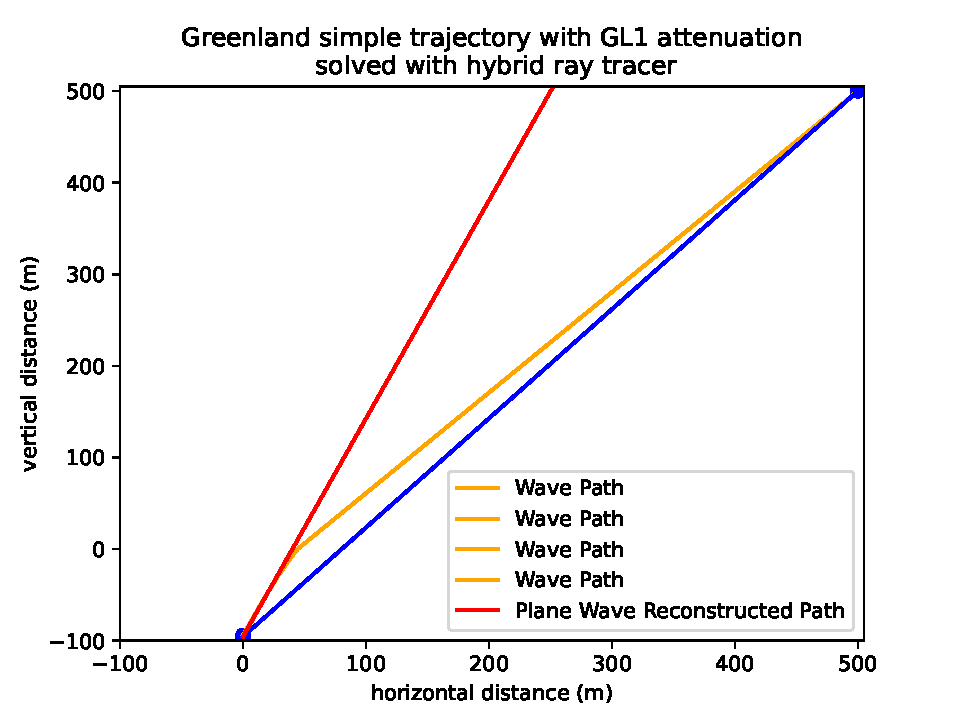
\includegraphics[width=0.7\textwidth]{WeatherBalloonPositionReconstruction.pdf}
	\caption{In blue is a straight line connecting the detector to the
	balloon. As can be seen, the balloon is too far away for a simple plane wave
	reconstruction, but using Snells law at the surface might mitigate the
	problem.}
	\label{fig:WeatherBalloonPositionReconstruction}
\end{figure}
Such a function is illustrated in figure \ref{fig:SummedCorrelation}.  For this
figure the modified hybrid ray tracing algorithm was used to simulate what the
difference in timing would be. 
As can be seen on the figure this function is minimal at a certain launch angle
$\theta_1$, we can use this angle and the height of the middle of the concerned
detectors to derive the path in the ice until it encounters the air-ice
boundary.  To know the path after this boundary we'll need the outgoing zenith
angle at the surface $\theta_2$ which can be calculated from Snell's law:
\begin{equation}
	n_1 \sin{\theta_1} = n_2 \sin{\theta_2} \implies  \theta_2 = \sin^{-1}\left(\frac{n_1}{n_2}\sin{\theta_1}\right)
\end{equation}
After doing this we have a linear function describing the path in air after it
passed the ice-air boundary layer.  If we evaluate this function at the height
of the balloon we then get the distance the reconstructed ray is away from the
balloon.  To find the index of refraction n we record this distance and redo
the procedure starting at the minimization of equation \ref{eqn:snellmin} for a
different index of refraction. After iterating through indices this way
we then have a list of corresponding distances to the balloon. The index
corresponding to the minimum in these distances is then the final result.
\begin{figure}
	\centering
	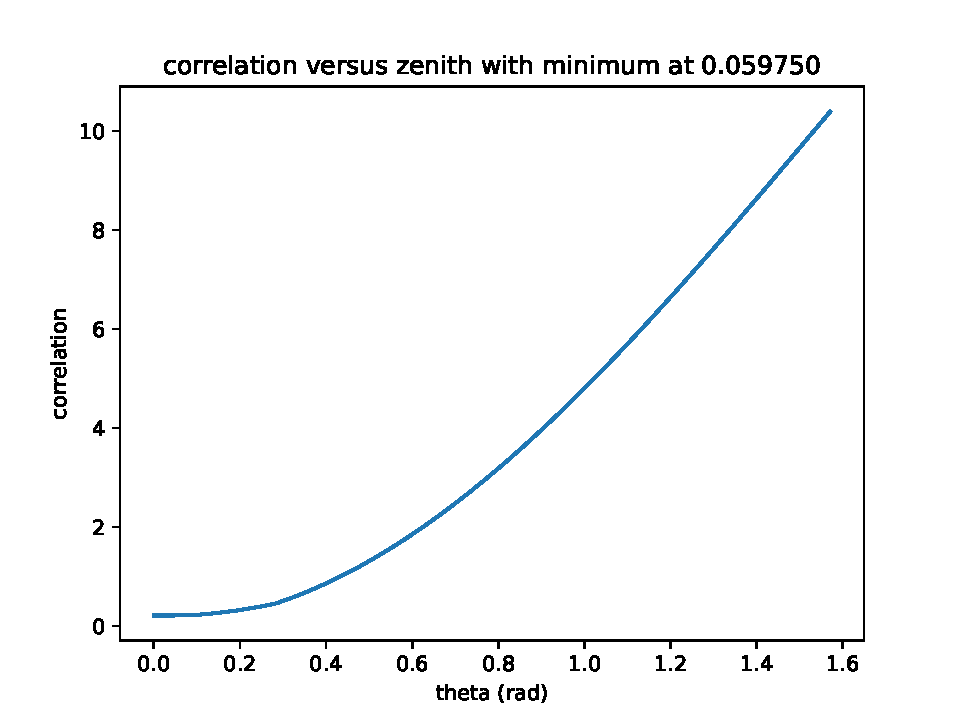
\includegraphics[width=0.8\textwidth]{SummedCorrelation.pdf}
	\caption{Example sum of the correlation functions, the ideal angle is located at the minimum of the curve}
	\label{fig:SummedCorrelation}
\end{figure}
\section{Is the goal feasible?}
\label{sec:feasible}
In the example reconstruction illustrated in figure
\ref{fig:WeatherBalloonPositionReconstruction} the difference in angle between
direct to balloon and plane wave reconstruction is quite big
($\approx 65\%$) but as the balloon gets closer to the detector this reduces
significantly. As previously mentioned out, our goal is to find the local index of refraction n by using the
plane wave reconstruction with the recorded timing and the positional data from
the weather balloon.

Now let's ask ourselves the question, within which angles should the
weather balloon fly for the data to be useful?  The
further the weather balloon is away (in the x direction) the bigger the zenith
angle with the detector, the less accurate the plane wave reconstruction.  So
which angles are acceptable? Note that not only angle but also height will eventually
play a role in the accuracy, the angle however gives a good starting point.

To determine the accuracy we vary the position of the weather balloon in the x direction (keeping the
height constant at 500m), simulate the ray path to channels 0 to 3 and then fit n
both via the simple plane wave reconstruction method explained out in section \ref{seq:SimplePW} and
the one using Snell's law explained in section \ref{seq:SnellPW}.
We then compare the indices we have fitted  to the
one we know from the model at that position.  We quantify the discrepancy
between the fitted and known index of refraction via the
\textit{systematic error}:
\begin{equation}
  \varepsilon\ (\%) = \frac{n_\text{fit} - n_{\text{exact}}}{n_{\text{exact}}}
\end{equation}
Carrying this out we get figure
\ref{fig:EpsilonIFODirect}. Both the Snell and simple plane wave method get
exponentially less accurate as the balloon moves further away.  If we wish the
systematic error to be within 1\% for the simple plane wave, the angle the
balloon makes with the middle of channels 0 to 3 needs to be less than 10°.
\begin{figure}
	\centering
	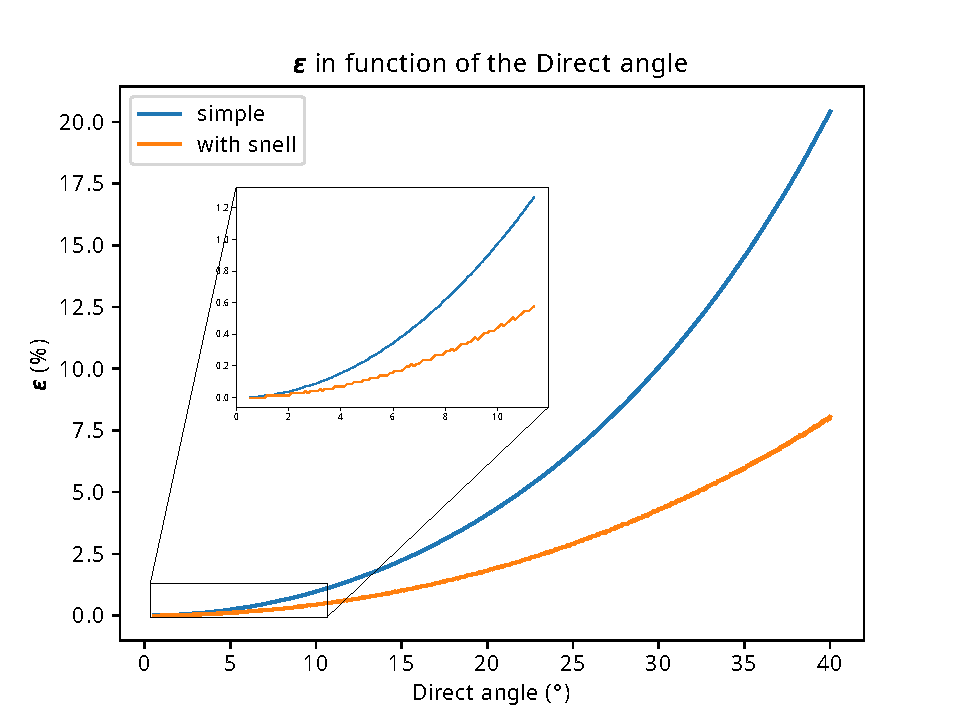
\includegraphics[width=0.8\textwidth]{EpsilonWithZoom.pdf}
	\caption{The accuracy of the plane wave reconstruction with the use of Snell's law at the surface is more 
  accurate but the simple plane wave method's accuracy is sufficient to make reliable
predictions for angles less than 10°. For small angles the simple reconstruction is preferred as no ice 
parameters need to be assumed.}
	\label{fig:EpsilonIFODirect}
\end{figure}

Now can we actually find moments when the balloon passes by a detector, making
an angle with the phased array of 10 degrees or less?  To figure this out we
looped over all the balloon positions recorded over the summer of 2022, more
particularly in the period 15/06/2022 - 30/09/2022 \footnote{The positional
data of the weather balloons was obtained from the \url{ftp1.esrl.noaa.gov}
website using the rno-g-sonde script of the official RNO-G github page.}, and
recorded the time intervals when they flew close enough.  To illustrate such a
trajectory, an example path of a balloon passing close enough to a detector is
shown in figure \ref{fig:ExampleBalloonPathCrossing12}.  The data shown in
appendices \ref{app:5Deg} and \ref{app:10Deg} respectively show $<5$° and
$<10$° encounters.
\newpage
\begin{figure}
  \centering
	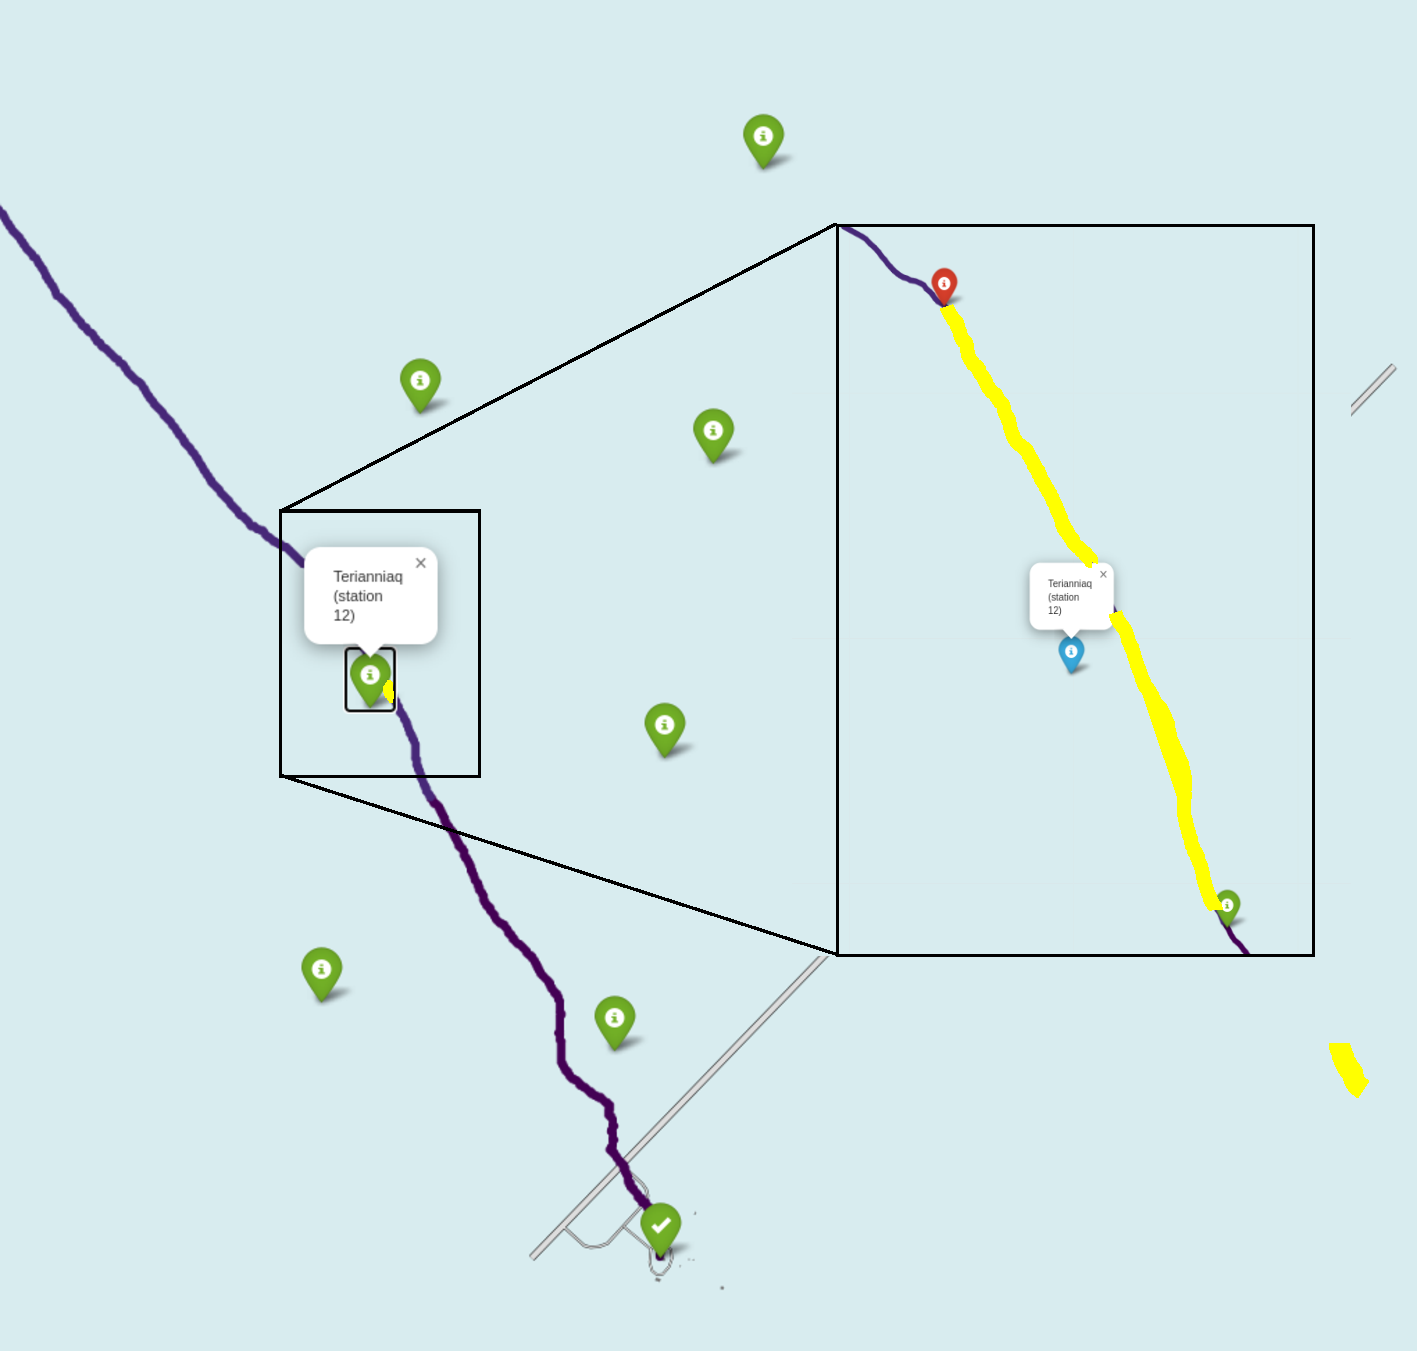
\includegraphics[width=0.5\textwidth]{BallonPathAllIllu.pdf}
  \caption{Path traced out by a weather balloon in purple released at 20/08/2022, in yellow you can see when it
  gets within 10° of detector 12. The green marks indicate the location of the various detectors.}
  \label{fig:ExampleBalloonPathCrossing12}
\end{figure}
\section{Fitting the index: Phased array}
Now that we know our goal to be feasible, let's analyze some data.  As we'll
start by just analyzing one event, let's take a reasonably good one for our analysis.

If we search in the DESY database
\footnote{\url{https://rnog-monitor.zeuthen.desy.de/}} within the calculated
time frames as listed in appendix \ref{app:5Deg} where the 403MHz signal coming from the
balloon is detected in the deep channels, an event recorded on the 24$^\text{th}$ of July stands
out; at 23:21:53 the balloon gets quite close to detector 11 and shows a clear
403MHz signal at the phased array in channels 0, 2 and 3, as shown for the
channels 2 and 3 in figure \ref{fig:freqs23}.

To use this event as to fit the index of refraction we built a program called FitN.py\cite{projects-mt}, 
which we'll now expound:
\subsubsection{Spatial data}
The first part we'll need to concern ourselves with is determining the relative
positions of everything. The balloon data file and the time when the event took
place are given, from these two both the latitudinal and longitudinal position
and the elevation of the balloon at the given time are determined, which we convert
to ENU (x,y,z) coordinates as to be able to use them. 

The locations of the various stations have also been determined and can be found 
on the official RNO-G github under "analysis-tools". 

Now that we have both the position of our balloon and station, 
let's simplify the calculations by setting the detector as the
origin i.e our new balloon position will be
\begin{equation}
  \mathbf{r}_{bs} = \mathbf{r}_b- \mathbf{r}_s
\end{equation}
With the subscript b denoting "balloon" and s "station".
As we might want to plot this later, due to the cylindrical symmetry of the
ice, we can rotate the coordinates to get rid of our y-axis. We can do
this by defining the radius:
\begin{equation}
  r := \sqrt{x_{bs}^2 + y_{bs}^2}
\end{equation}
And redefining our relative position as
\begin{equation}
  \mathbf{r} = 
  \begin{bmatrix}
  r \\
  0 \\
  z_{bs}
  \end{bmatrix}
\end{equation}
We don't have the position of our individual channels yet, only of the station
itself. The relative position of these\footnote{relative to the detector} can
however also be obtained and as we chose our station to be the center of the
coordinate system, these relative positions are absolute positions of the
channels in our frame of reference. Using these, it thus doesn't matter where
the position of the station was defined.

\subsubsection{Signal analysis and initial guesses}
Now that we have the positions of both the balloon and the channels, let's
analyze the data. The data for a particular channel from a
recorded event (here event 12397 of run 1034) is stored in a channel object,
from this object we can get the recorded voltages and times during this event.
These recorded voltages can be Fourrier transformed to get the recorded
frequency spectrum.  We know that the signal sent out by the weather balloon is
a sine wave with a frequency of 403MHz; as the data is measured in nanoseconds
the frequency is:
\begin{equation}
	f = 403\text{MHz} = 403\times 10^{-3} \frac{1}{\text{ns}}
\end{equation}
The recorded spectrum of channels 2 and 3 is given in figure \ref{fig:freqs23}, for 
which we previously mentioned the spike at 0.403GHz.
\begin{figure}
	\begin{minipage}{0.49\textwidth}
		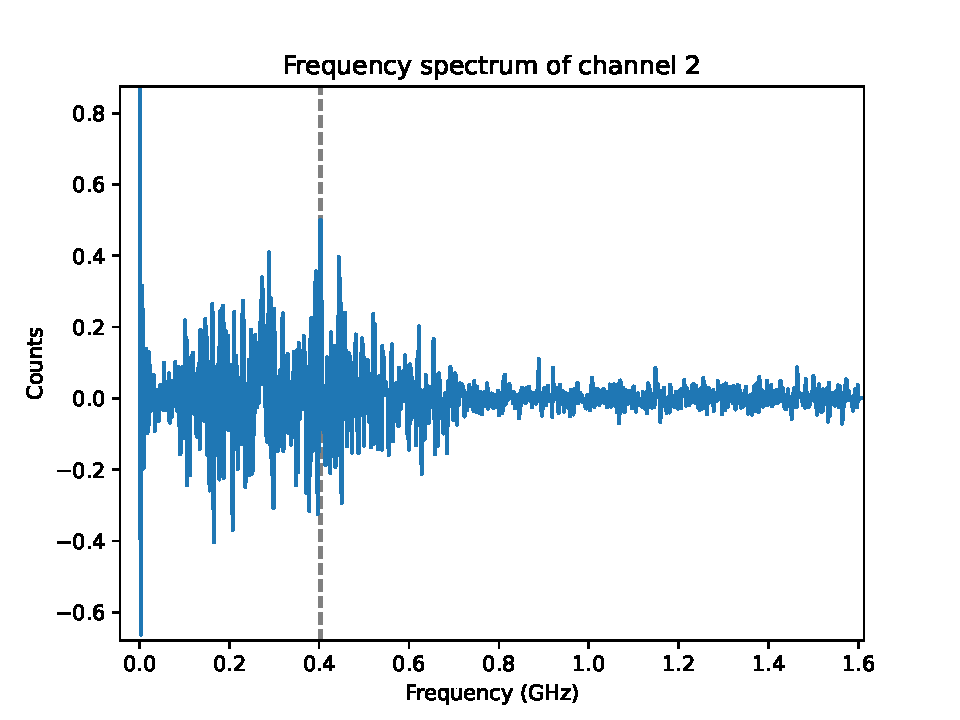
\includegraphics[width=\textwidth]{figures/2-freq.pdf}
	\end{minipage}
	\begin{minipage}{0.49\textwidth}
		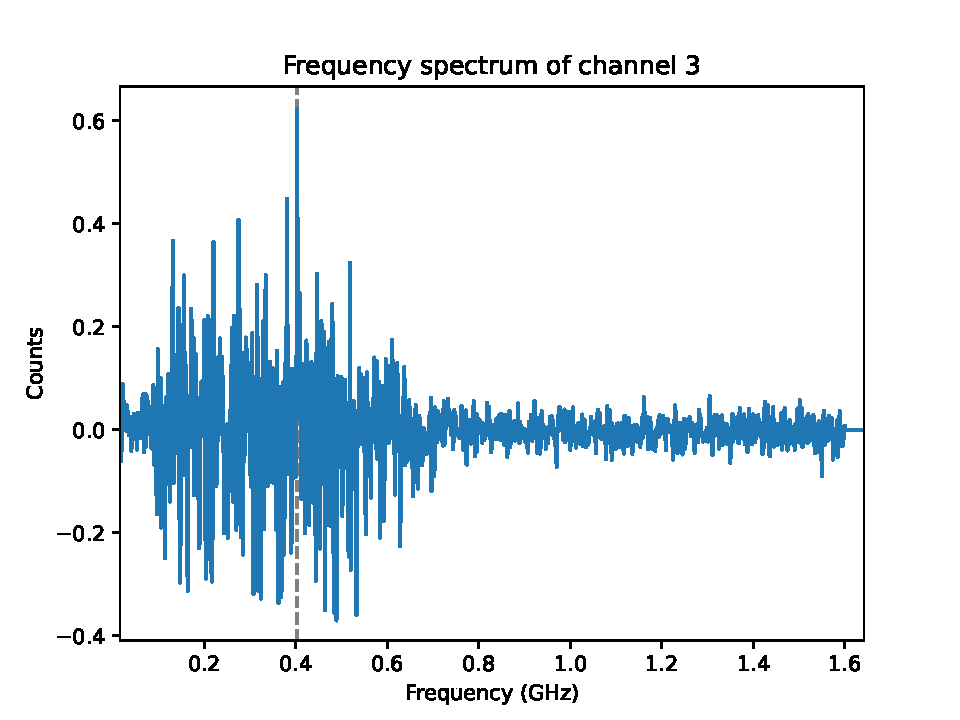
\includegraphics[width=\textwidth]{figures/3-freq.pdf}
	\end{minipage}
	\caption{recorded frequencies on detector 11 at 2022/07/24 23:21:53, clear spikes at 0.403GHz are visible}
	\label{fig:freqs23}
\end{figure}
Now note that on this figure it's shown that there are signals with frequencies
both below 0.15GHz and above 0.6GHz, these can be left out as the Vpol is
defined to be most responsive only in the range 0.15GHz to 0.6GHz
\cite{Aguilar_2021}. To filter out these frequencies we'll pass the signal through a virtual
butterworth bandpass filter.

Now that we have filtered our data we'd also like to increase the accuracy in
timing, to this end we'll resample the signal\footnote{Resampling is the process of
changing the sampling rate of a discrete signal to obtain a new discrete
representation of the underlying continuous signal}. We'll upsample towards 10GHz
increasing our timely accuracy from 0.3125ns to 0.1ns, this is possible as the
full Nyquist-sampled waveforms are stored\cite{Allison_2019}.  As the timely accuracy
is now 0.1ns, the error on a time difference between channels is 0.2ns. So
$\delta t_{ij}=0.2$ns as explained in section \ref{seq:SimplePW}.

After this cleaning of
our data (by filtering and upsampling) we have a voltage response with an example 
shown for channel 0 in figure \ref{fig:VoltageAfterFilter}, we wish to find a sine
wave coming from the weather balloon in this signal.
\begin{figure}
	\centering
	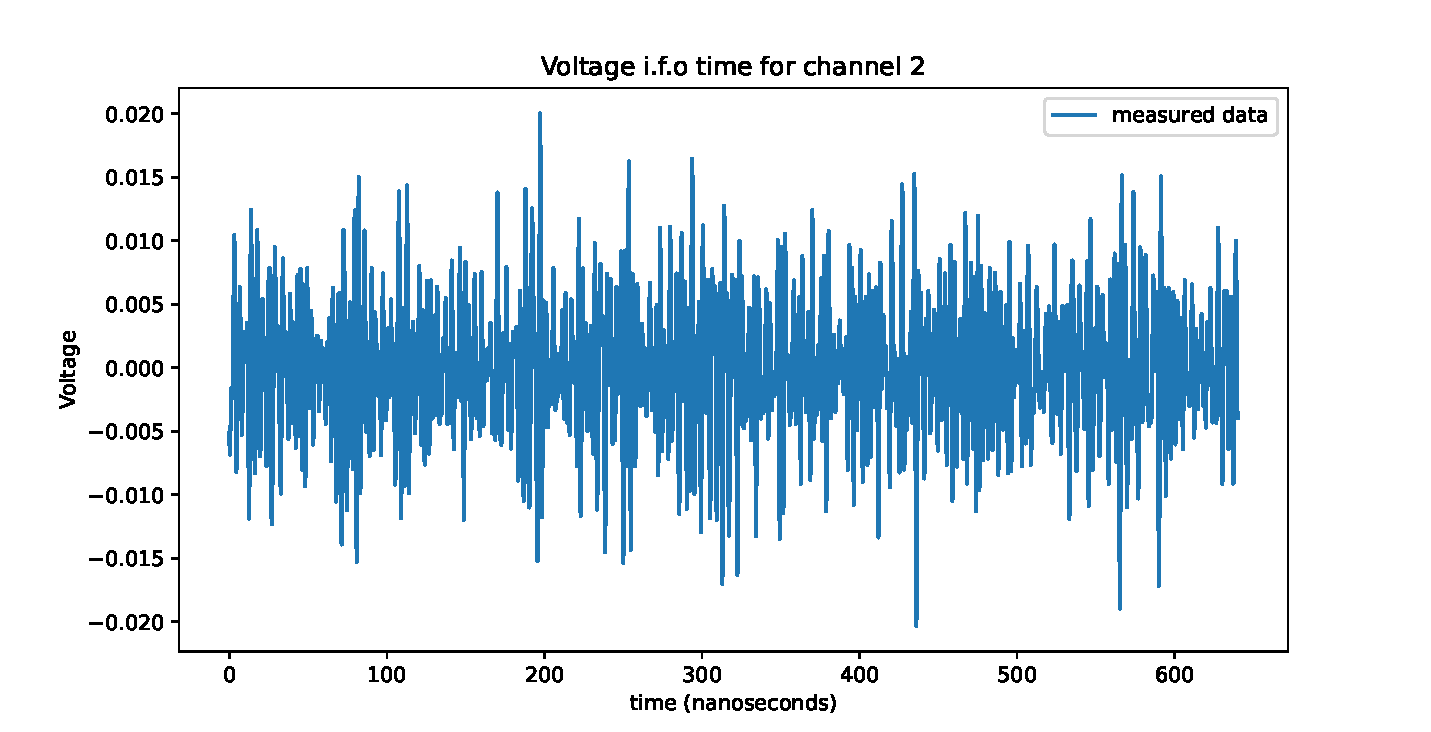
\includegraphics[width=\textwidth]{figures/VoltageAfterFilter.pdf}
	\caption{Recorded voltage i.f.o time in vpol antenna 2 after upsampling and passing through the butterworth filter, herein we'll need to find a sinusoidal signal.}
	\label{fig:VoltageAfterFilter}
\end{figure}
To find a sine wave herein, and thus find out the timing of our signal, we'll
make use of a method called \textit{cross correlation}, whereby we move a
template over our data, returning a high value if the data and template line up
and a low value if they don't.

We thus need a template to correlate with the data. The template we'll be choosing is
of course the sine function but it's important to notice that the channel has a
certain sampling rate, namely now after upsampling, 10GHz. 

Our template sine which we'll correlate to the data will also need to have this
sampling rate, meaning that it needs to be step wise defined with spaces of
0.1ns. Next we'll also need to give the sine a certain amplitude, as we don't
have a system for finding this let's assume an amplitude $A =0.007$ 
(this shouldn't impact the result).  Our template thus looks like this:
\begin{equation}
	\mathcal{S} = A\cdot\sin(\omega t) 
\end{equation}
with
\begin{equation}
	\omega = 2\pi f
\end{equation}
With f the frequency of the balloon signal, 0.403GHz and $t$ an array going
from 0 to $3/f$ as to be able to fit 3 periods. The
cross-correlation is done by moving the signal with steps of $\Delta t = 0.1$ns,
an illustration of this procedure is shown in figure \ref{fig:SineCorrFull}. Mathematically this
amounts to evaluating\cite{Bracewell1966TheFT}:
\begin{equation}
  (f\star g)(\tau) \delequal \int_{-\infty}^\infty f(t)g(t+\tau)dt
\end{equation}
With f(t) the recorded signal and g(t) the sine wave template\footnote{$\delequal$ means "equal by definition"}.

\begin{figure}
	\centering
	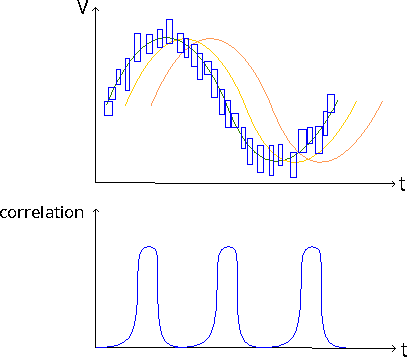
\includegraphics[width=0.8\textwidth]{figures/SineDataCorrFull.pdf}
	\caption{How correlating a sine with data leads to periodic peaks in the correlation function}
	\label{fig:SineCorrFull}
\end{figure}
In reality the data is a bit less perfect and after doing this correlation
procedure on the real data we get what's (partially) shown in figure \ref{fig:CorrCh2}.
\begin{figure}
	\centering
	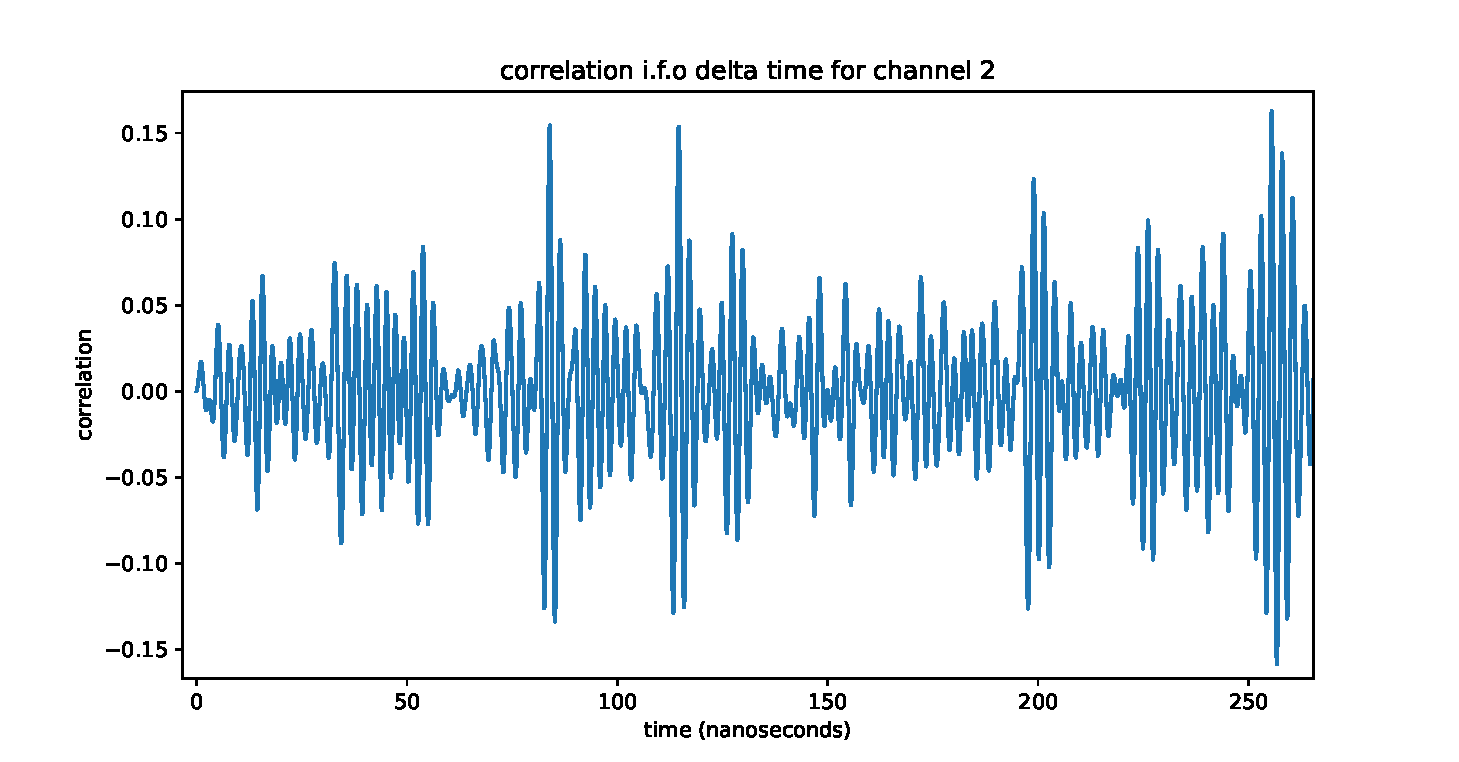
\includegraphics[width=\textwidth]{figures/CorrelationCh2.pdf}
	\caption{The correlation is less clear than in the illustration but still shows the periodicity of the sinusoidal signal}
	\label{fig:CorrCh2}
\end{figure}
Herein the peaks represent the maximal correlation, if we now do the same for
channel 3 we have two correlation functions, if we crosscorrelate these with
each other we'll get the difference in timing between the channels.  This is
easy to comprehend after taking a look at the illustration shown in figure
\ref{fig:IlluCorr}. 
\begin{figure}
  \centering
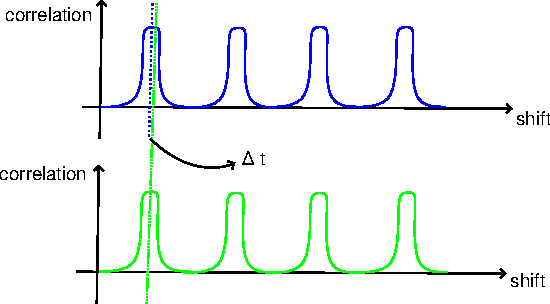
\includegraphics[width=0.8\textwidth]{figures/IlluCorr.pdf}
\caption{Crosscorrelating two crosscorrelated functions gives peaks at the differences in timing}
	\label{fig:IlluCorr}
\end{figure}
What this cross-correlation of cross-correlated functions then looks like is partially shown
in figure \ref{fig:CrossCrossCorr}, the negative offset is caused by us accounting for cable
delay. Note that multiple peak correlations are present. To find out which peak
is the actual observed time difference, we'll need to analyze the physics of the problem.
\begin{figure}
  \centering
  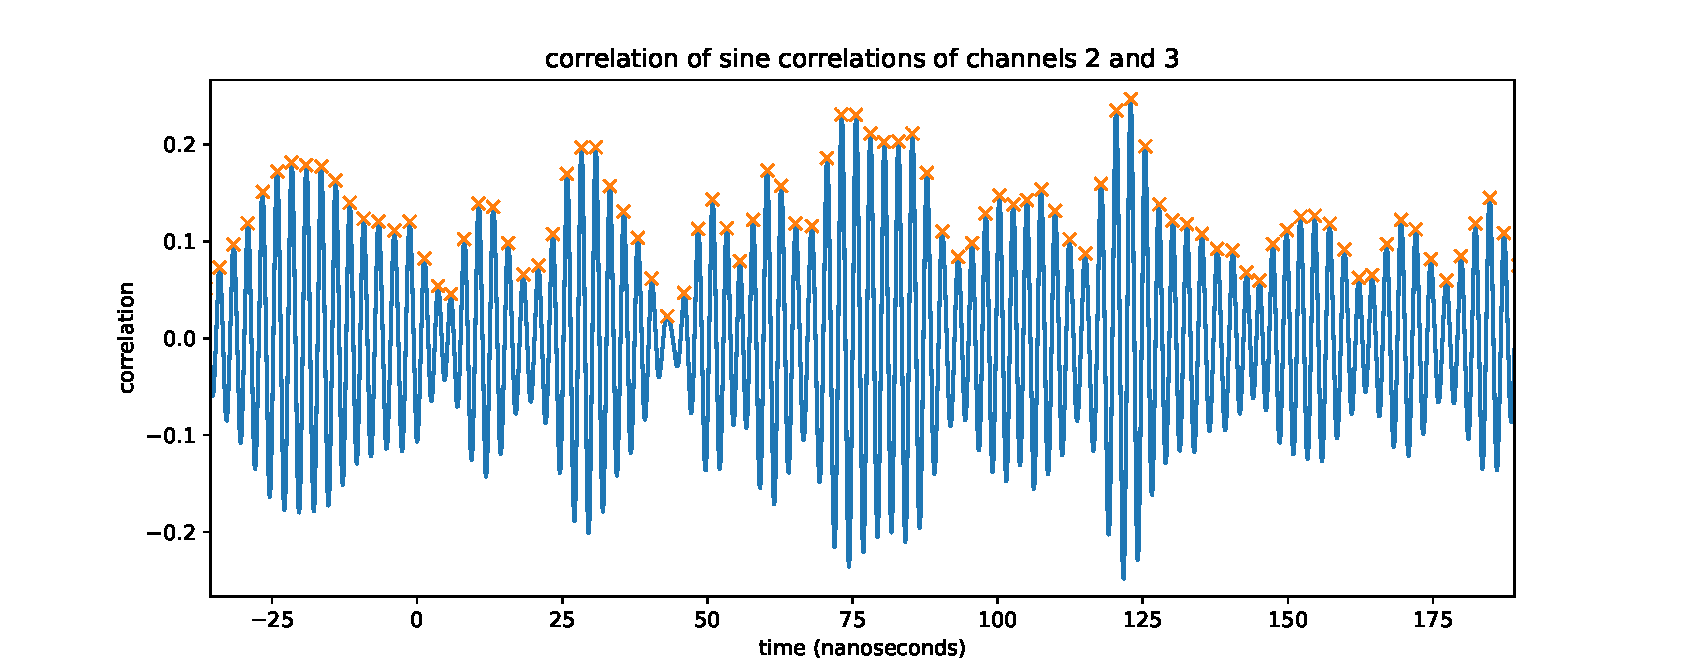
\includegraphics[width=\textwidth]{figures/CrossCrossCorr.pdf}
  \caption{There are multiple peaks present but only one peak is the physically possible difference in timing. In this case (channels 2 and 3)
  it's the third peak counting from t=0}
	\label{fig:CrossCrossCorr}
\end{figure}
Our signal is sinusoidal with a frequency of 0.403GHz, locally our index of refraction should be around 1.7,
meaning that our wavelength should be:
\begin{equation}
  \lambda = \frac{v}{f} = \frac{c}{nf} \approx 0.44m
\end{equation}
This wavelength is longer than the distance between the individual channels, meaning that if the top
of the sinusoidal wave gets detected in channel 2, then the sinusoidal wave gets detected in
channel 3 $\frac{1m}{0.44m} \approx 2.3$ wavelengths later. So we expect at least two peaks to 
have gone by until the same sinusoidal wave as observed in channel 2 gets detected in channel 3.
We thus have to search for the third peak (starting from t=0) in this case, similarly for detectors 0 and 3
which are spaced 3 meters apart we'll need to look at peak number $\lceil\frac{3m}{0.44m}\rceil = 7$.
And for completeness sake, for channels spaced 2 meters apart we'll need to look at peak 
$\lceil\frac{2m}{0.44m}\rceil = 5$. In reality however, it is easier to just simulate the time differences
and look in that neighborhood.

\subsubsection{Fitting n and finding its error}
Now that we have the differences in timing between the individual channels and their error, the
angle the balloon makes with the detector and the distance between the individual channels
all that's left to do is minimize function f as defined in equation \ref{eqn:PlaneWave} and
calculate the error. Doing the full procedure we get:
\begin{center}
\begin{tabular}{||c c c c c c||}
 \hline
 Depth (m) & Station id & channels & Run:Event & n$_\text{exponential}$ & n$_\text{fit}$\\ [0.5ex]
 \hline\hline
 94.518 & 11 & 0\&2\&3 & 1034:12397 & 1.7397 & 1.724 $\pm$ 0.014 $\pm$ 0.047 \\
 \hline
\end{tabular}
\end{center}
With the first error indicating the systematic error and the second one the error found through
error analysis. After varying both the positional and timely error it seems that the error on position is the biggest
contributing factor.

\section{Phased array and channels 5-7}
The event we'll now analyze is recorded in detector 21 at the 26$^\text{th}$ of July
11:18:41 and falls within the $<5$° mark, the balloon signal gets detected
by both the phased array and channels 5 to 7.

Channels 5 to 7 lie at a very interesting depth as, looking at 
the density versus depth data shown in figure \ref{fig:DensityMeasurements},
here (40-80m depth) the difference between the density measurements and the single
exponential model shows the largest deviations. 

As channels 5 to 7 are spaced quite far apart we can do the plane wave fitting 
for two channels at a time, still keeping the error quite small. The results are given below:
\begin{center}
\begin{tabular}{||c c c c c c||}
 \hline
 Depth (m) & Station id & channels & Run:Event & n$_\text{exponential}$ & n$_\text{fit}$\\ 
 \hline\hline
 48.155 & 21 & 6\&7 & 1441:117 & 1.6400 & 1.632 $\pm$ 0.00128 $\pm$ 0.00472\\
 58.38 & 21 & 5\&7 & 1441:117 & 1.6736 & 1.66632 $\pm$ 0.00226 $\pm$ 0.00233 \\
 58.24 & 21 & 5\&6\&7 & 1441:117 & 1.67321 & 1.66553 $\pm$ 0.00167 $\pm$ 0.00350 \\
 68.2 & 21 & 5\&6 & 1441:117 & 1.6983 & 1.69329 $\pm$0.00199$\pm$0.00460 \\
 93.865 & 21 & 0\&1\&2\&3 & 1441:117 & 1.73896 & 1.71366$\pm$0.00287$\pm$0.05641\\
 \hline
\end{tabular}
\end{center}
\begin{figure}
	\centering
	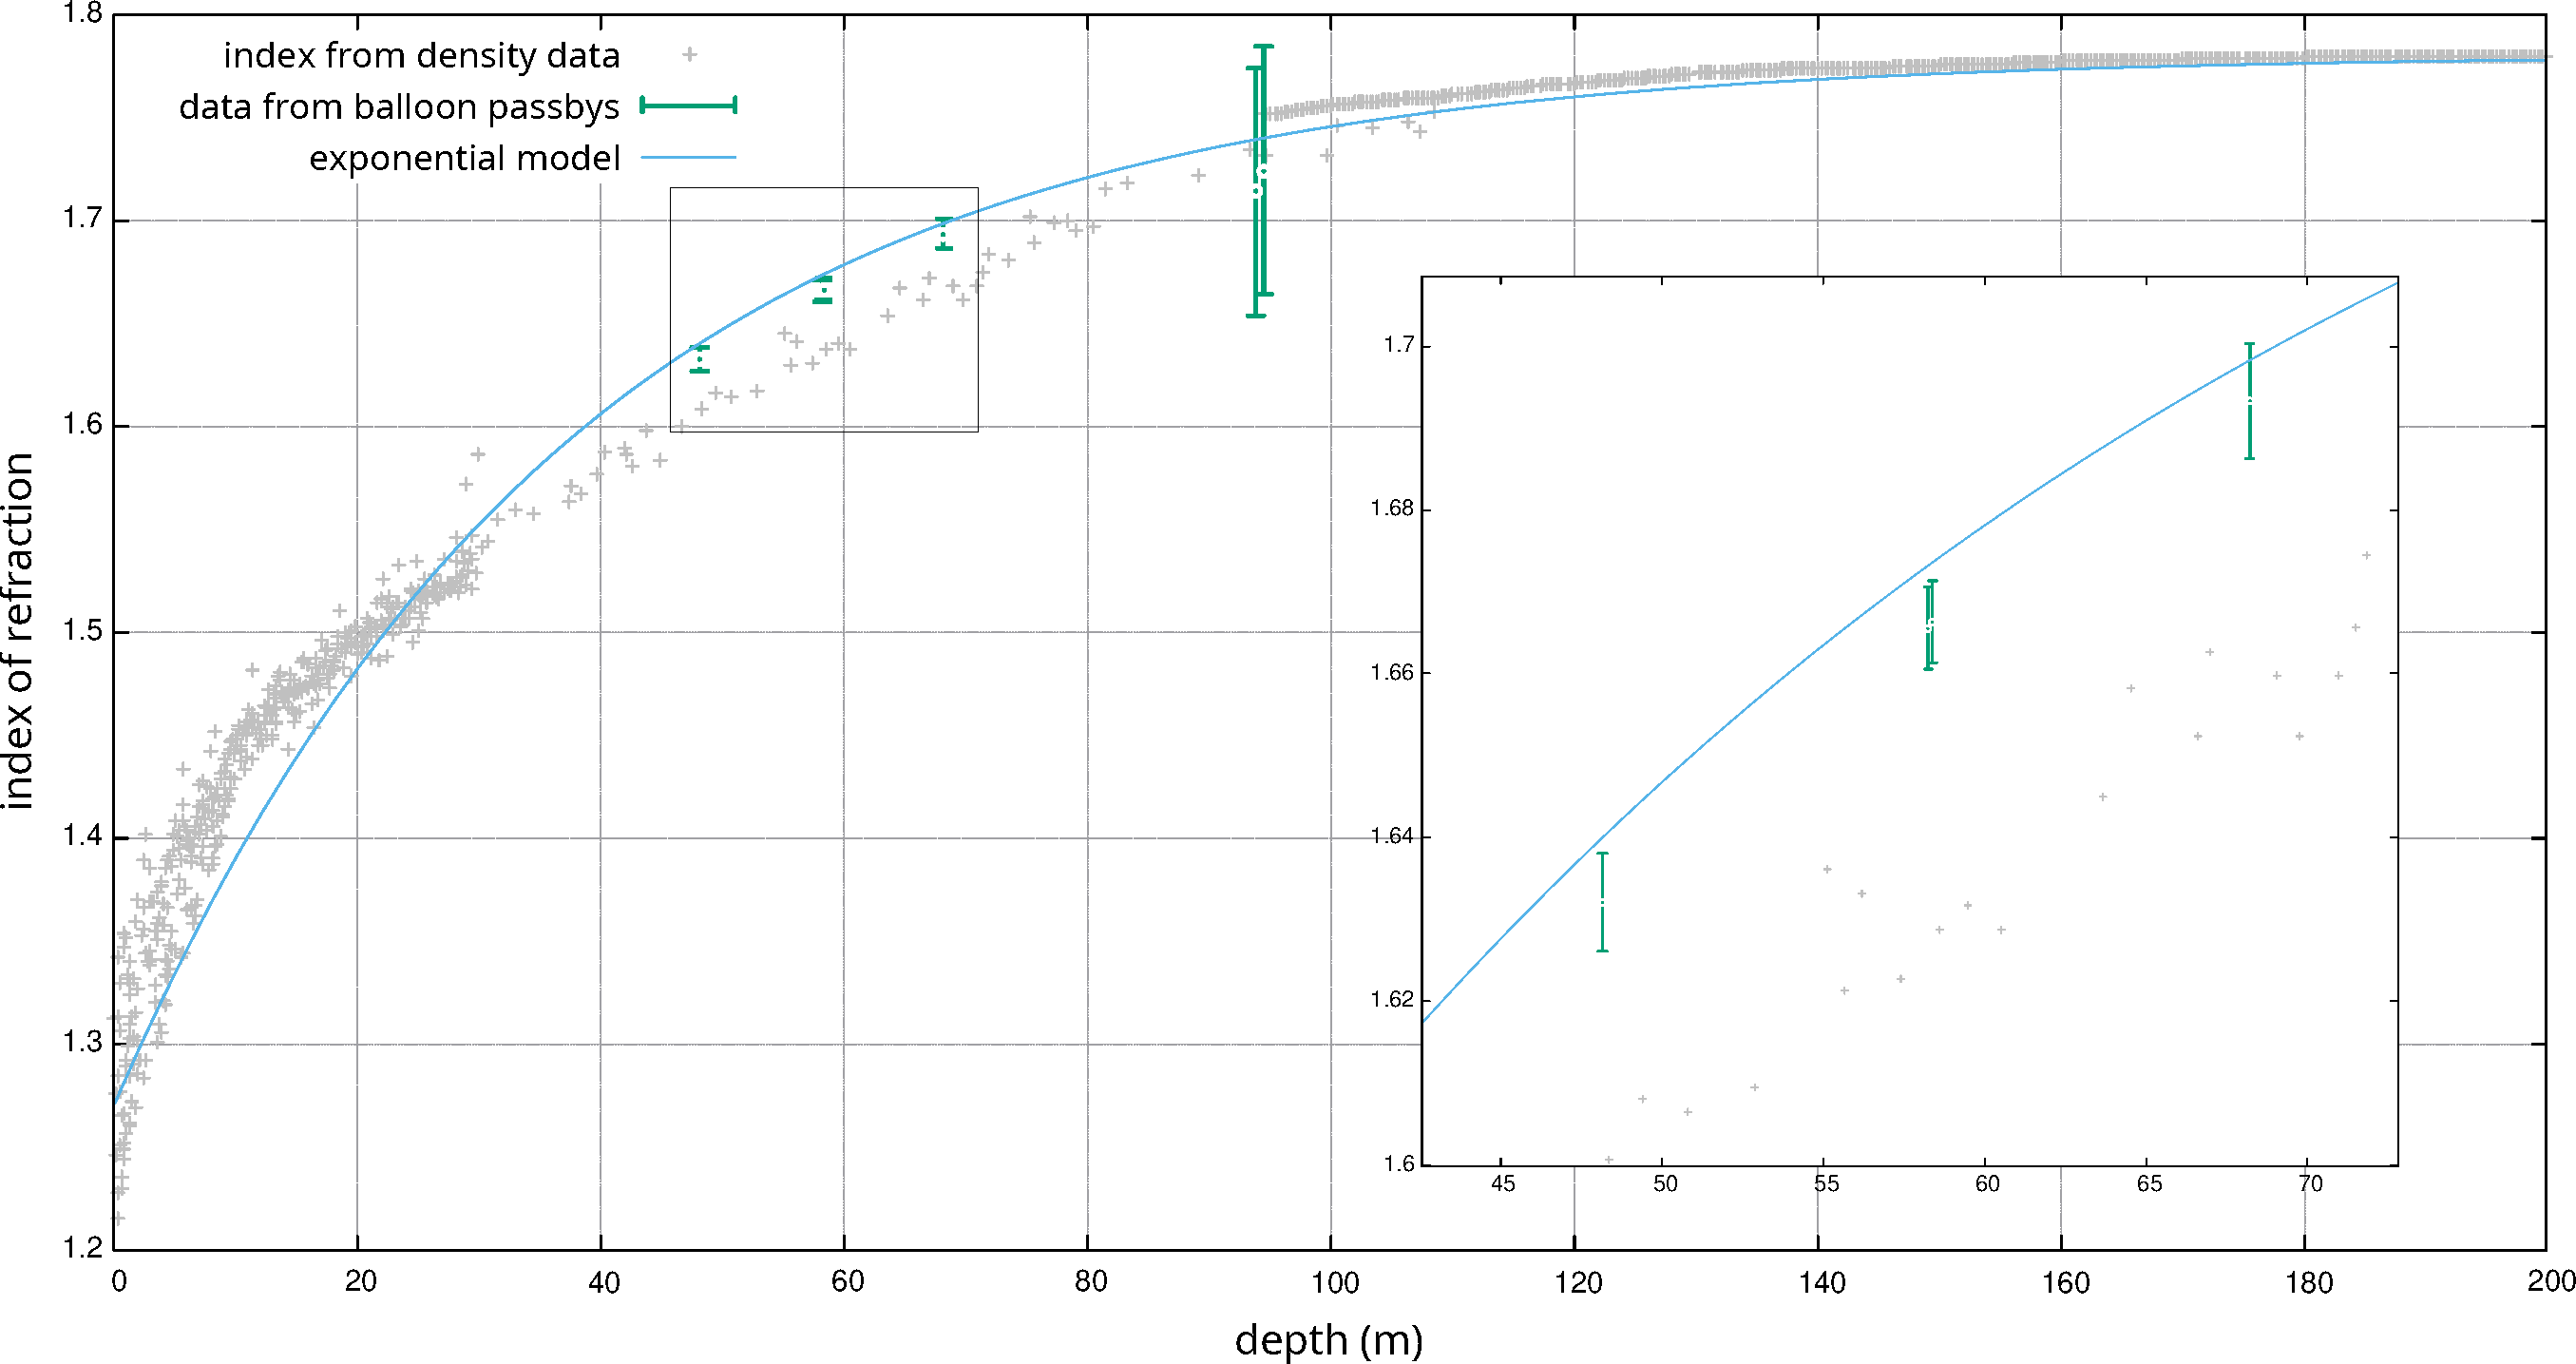
\includegraphics[width=\textwidth]{figures/ResultWithZoom.pdf}
  \caption{Even though the error bars are quite big, all values found within this chapter lie under the single exponential, 
    which is especially clear at the phased array depths where the measurements
    are below both the exponential model and the data from the converted densities.}
	\label{fig:Results}
\end{figure}
\section{Evaluation of the results}
All the fits that were found are visually shown in figure \ref{fig:Results},  together
with the index found by converting the density data through the linear index-density relation
($n(z) \approx 1 + 0.845\rho(z)$) and the exponential model\footnote{A bigger version can also be found in appendix \ref{app:ExtraFigures}}.
Note that all of the indices that have been found have a value below the
exponential model's, more closely to the converted density data.
Even though the error is quite big these results could raise some
suspicion on the validity of the exponential model and might indicate
that it's needed to measure the whole index-depth profile.

Now note that the measurements on depths 40-80m don't fully agree with the density data, 
this could be caused by one of the following reasons:
\begin{itemize}
	\item The density measurements aren't accurate enough
	\item The index isn't fully linear at every depth
	\item The fit isn't accurate enough and thus the error bars are underestimated
\end{itemize}
The density measurements do actually show quite a lot of spread for
nearly the same values so there might be a problem there. There are
also not that many recorded measurements in the 40-100m region and no reported
uncertainties which makes the data less trustworthy.  

As for the linearity relation, it has been extensively studied in the literature
\cite{KOVACS1995245} and there seem to be multiple relationships reported,
all however were linear. Another possible relation is e.g
\begin{equation}
  n(z) \approx 1 + 0.77\rho(z)
\end{equation}
How our data correlates with this relation is shown in figure
\ref{fig:ResultsOtherLinear}, but this doesn't seem to heavily impact the
distance from the density converted data and our measurements.

Lastly as channels 5-7 are spaced quite far apart, the plane wave reconstruction
might not be fully viable and the assumption that the incoming angle is the same for
all channels not fully correct. But as the balloon is really close during this event
we think that this contribution is negligible and the results should be somewhat viable.

It might thus be needed to measure the index-depth relation directly and so
obtain an experiment-based ice model.


% =====================================================================
% End matter
% =====================================================================

\chapter*{Conclusion}
\addcontentsline{toc}{chapter}{Conclusion}
The hybrid ray tracer developed over the course of this thesis and reported in
chapter \ref{chapter:hybrid} was a success, not only is it more accurate than
it's predecessors, as shown in figures \ref{fig:acchyb} and \ref{fig:accit},
 but it's also faster by about 34\%.  The accuracy of the ray tracer also
makes it perfectly suitable for very fine precision simulations as used within
the Balloon radio wave measurements.

The use of weather balloons to estimate the index of refraction as
was reported in \ref{chap:WB} was also done successfully 
yielding the following data:
\begin{center}
\begin{tabular}{||c c c c c c||}
 \hline
 Depth (m) & Station id & channels & Run:Event & n$_\text{exponential}$ & n$_\text{fit}$\\ [0.5ex]
 \hline\hline
 -94.518 & 11 & 0\&2\&3 & 1034:12397 & 1.7397 & 1.7045 $\pm$ 0.006 \\
 \hline
\end{tabular}
\end{center}
And visually shown as the data in blue on figure \ref{fig:IndexVSDepth.pdf},
it clearly shows a big discrepancy with the exponential model.
We reason that this clearly shows that there's a need to investigate
the index-depth relation further as the wave propagation, and thus
neutrino reconstruction, are heavily dependent on the ice model.

Note that there was only one event in the phased array that was analysed, this 
is because the occasions of when a balloon passes close enough to a detector
and when the signal is measurable in the deep array are very few.

As there are a multitude of events (as can be found in appendices
\ref{app:5Deg} and \ref{app:10Deg} but only finite time to analyze each and
every one, this code is also made public
\href{https://github.com/arthuradriaens-code/projects-mt.git}{here} as to make
it easy to improve on this work.  Especially interesting might be events where
$\epsilon$ is negligible (the balloon is really close) at the phased array and
as such is the plane wave reconstruction a near perfect representation of the
actual wave.
\newpage
As this method seems to be a viable way of measuring the index of refraction,
it might be a good idea to have a more controllable radio wave source fly
closer to the detectors to make more accurate measurements, e.g an
autonomous\footnote{as to not have it need a radio controller, causing RF
interference on top of the one coming from the engine and also as autonomous
GNSS positioning is always more accurate than human steering} drone with an
antenna strapped to it or just some form of stationed antenna.  

It might also be a good idea to make the signal easier to fit, as the currently
used signal has quite a short wavelength (0.403GHz) we have to guess when the 
signal roughly arrives. If we have, say an AM signal, we wouldn't have to assume
the rough arrival time of the signal, thus reducing the possible error on timing.

In the ideal case, as has been done in the South Polar firn\cite{kravchenko_besson_meyers_2004}, we'd want some immobile close source and a phased array which we'll
move down every couple of measurements, thus obtaining an index-depth profile
using direct measurements. This might be carried out e.g during deployment
of a new station's power string.

\appendix
\chapter{List of abbreviations}
\begin{itemize}
\item \textbf{AM}: \textbf{A}mplitude \textbf{M}odulated
\item \textbf{AGN}: \textbf{A}ctive \textbf{G}alactic \textbf{N}ucleus
\item \textbf{CMB}: \textbf{C}osmic \textbf{M}icrowave \textbf{B}ackground
\item \textbf{DAQ}: \textbf{D}ata \textbf{AQ}uisition system
\item \textbf{DnR}: \textbf{D}irect a\textbf{N}d \textbf{R}efracted
\item \textbf{DSNB}: \textbf{D}iffuse \textbf{S}upernova \textbf{N}eutrino \textbf{B}ackground
\item \textbf{FFT} \textbf{F}ast \textbf{F}ourrier \textbf{T}ransform
\item \textbf{GRBs}: \textbf{G}amma-\textbf{R}ay \textbf{B}ursts
\item \textbf{RADIANT}: \textbf{RA}dio \textbf{DI}gitizer and \textbf{A}uxiliary \textbf{N}eutrino \textbf{T}rigger
\item \textbf{RNO-G}: \textbf{R}adio \textbf{N}eutrino \textbf{O}bservatory in \textbf{G}reenland
\item \textbf{RF}: \textbf{R}adio \textbf{F}requency
\item \textbf{UHE}: \textbf{U}ltra \textbf{H}igh \textbf{E}nergy 
\item \textbf{UHECRs}: \textbf{U}ltra \textbf{H}igh \textbf{E}nergy \textbf{C}osmic \textbf{R}ay\textbf{s}
\end{itemize}
\chapter{Extra Figures}
\label{app:ExtraFigures}
\begin{figure}[h]
	\centering
	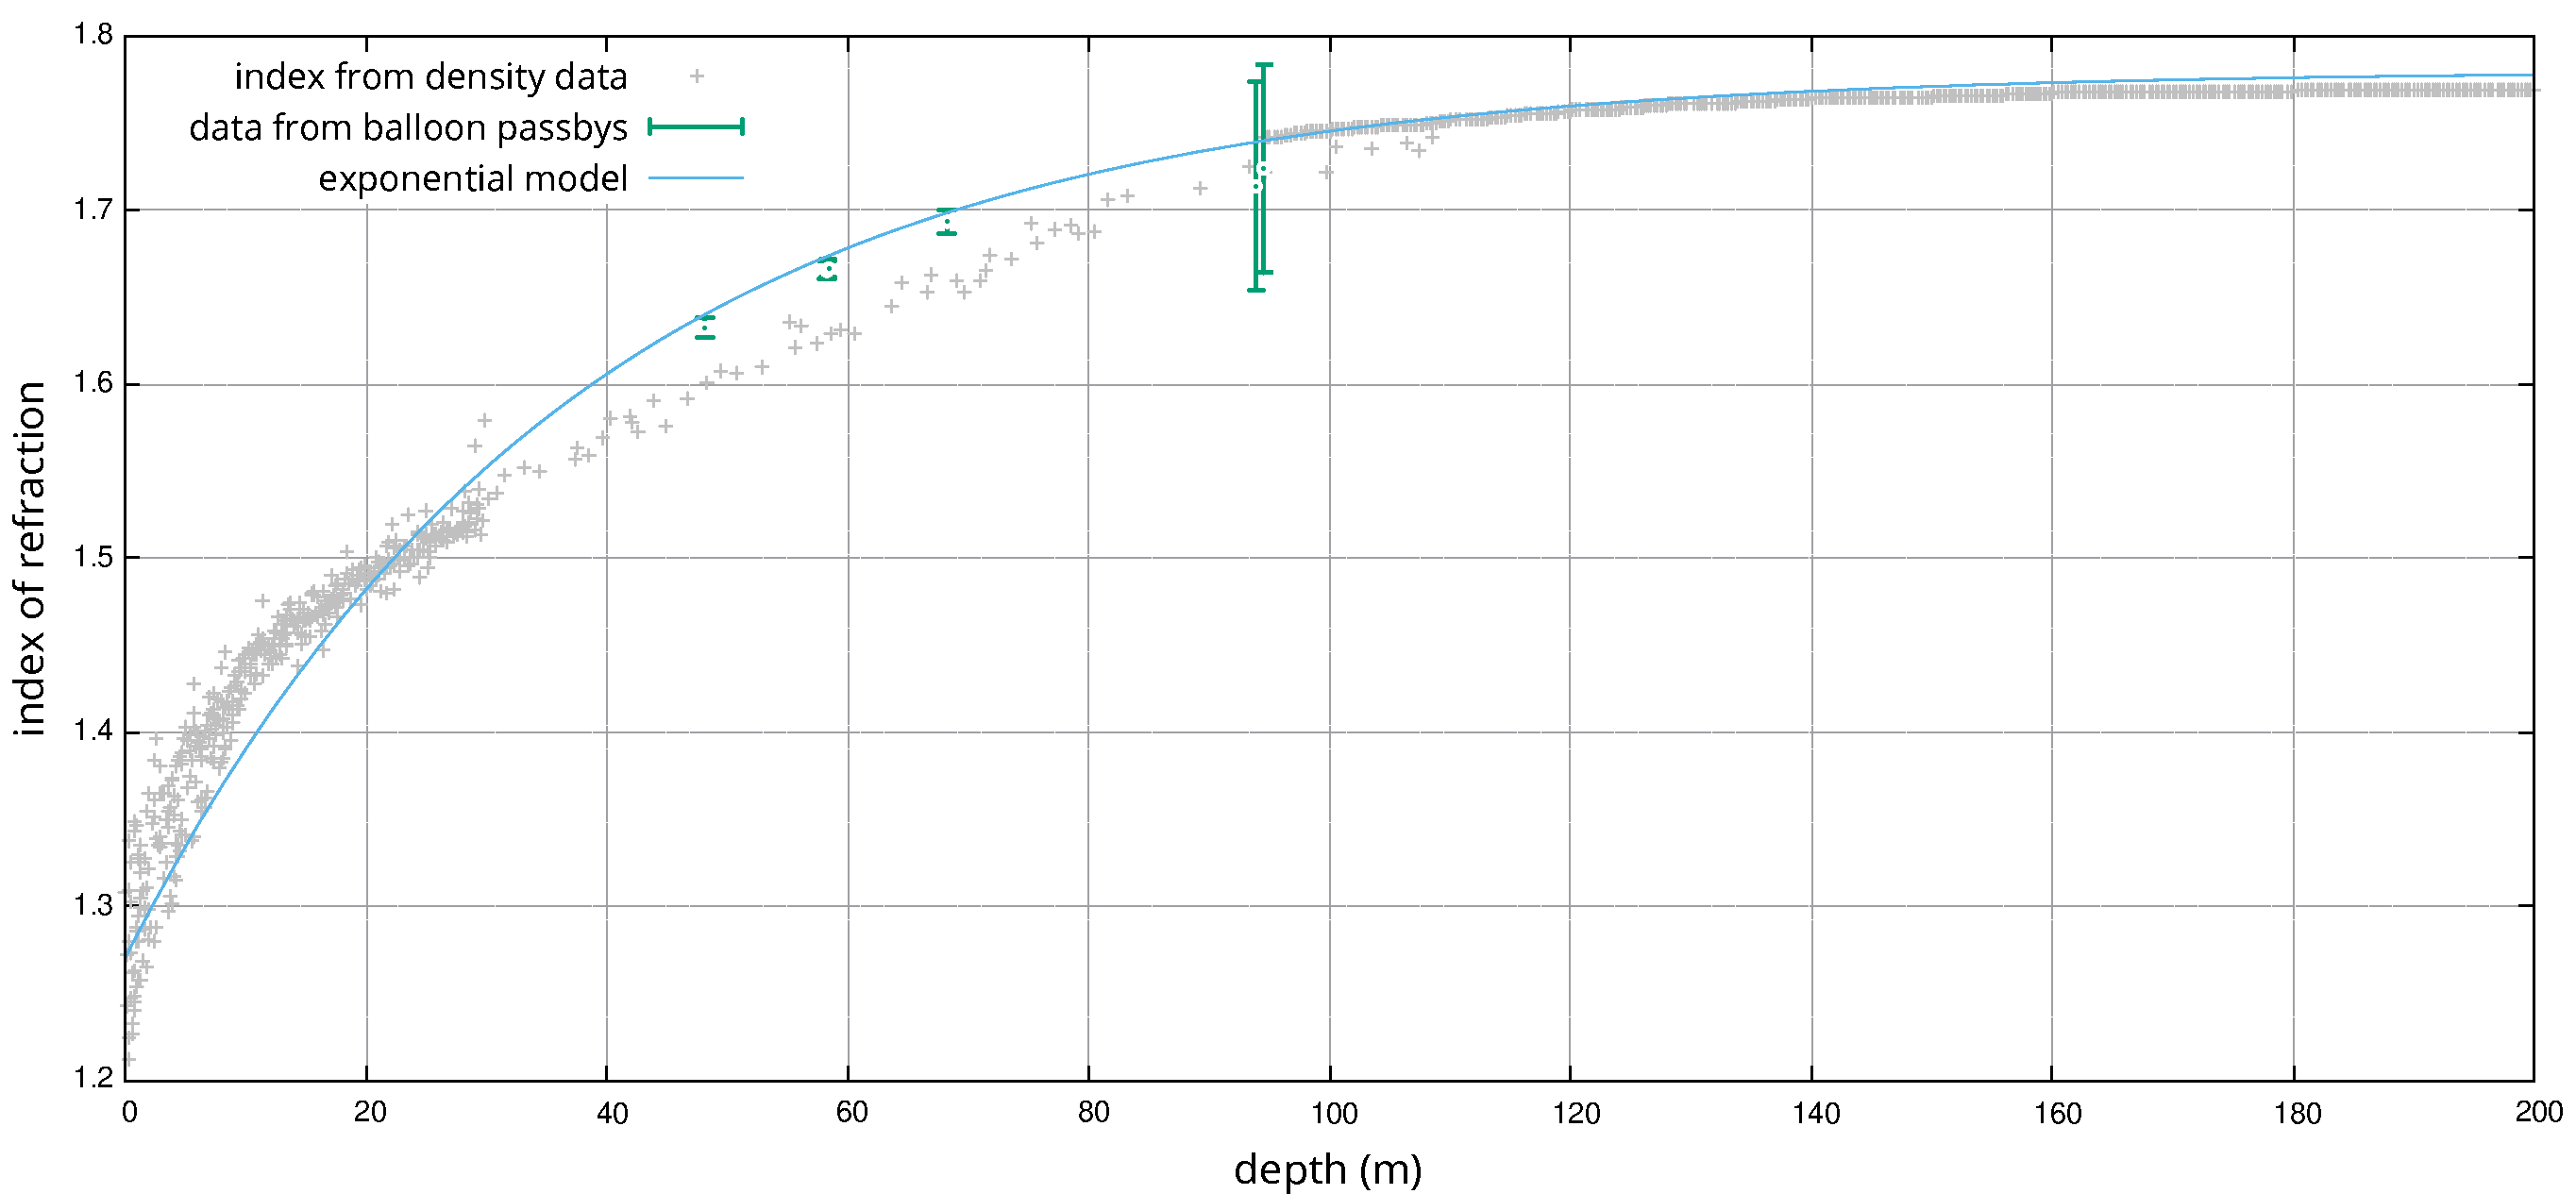
\includegraphics[width=\textwidth]{figures/ResultsOtherLinear.pdf}
  \caption{Changing the linear index-density relation from $n(z) = 1+0.78\rho(z)$ to $n(z) = 1+0.77\rho(z)$ (shown here) seems
to make our phased array measurements lie closer to the density data}
	\label{fig:ResultsOtherLinear}
\end{figure}
\begin{figure}
	\centering
	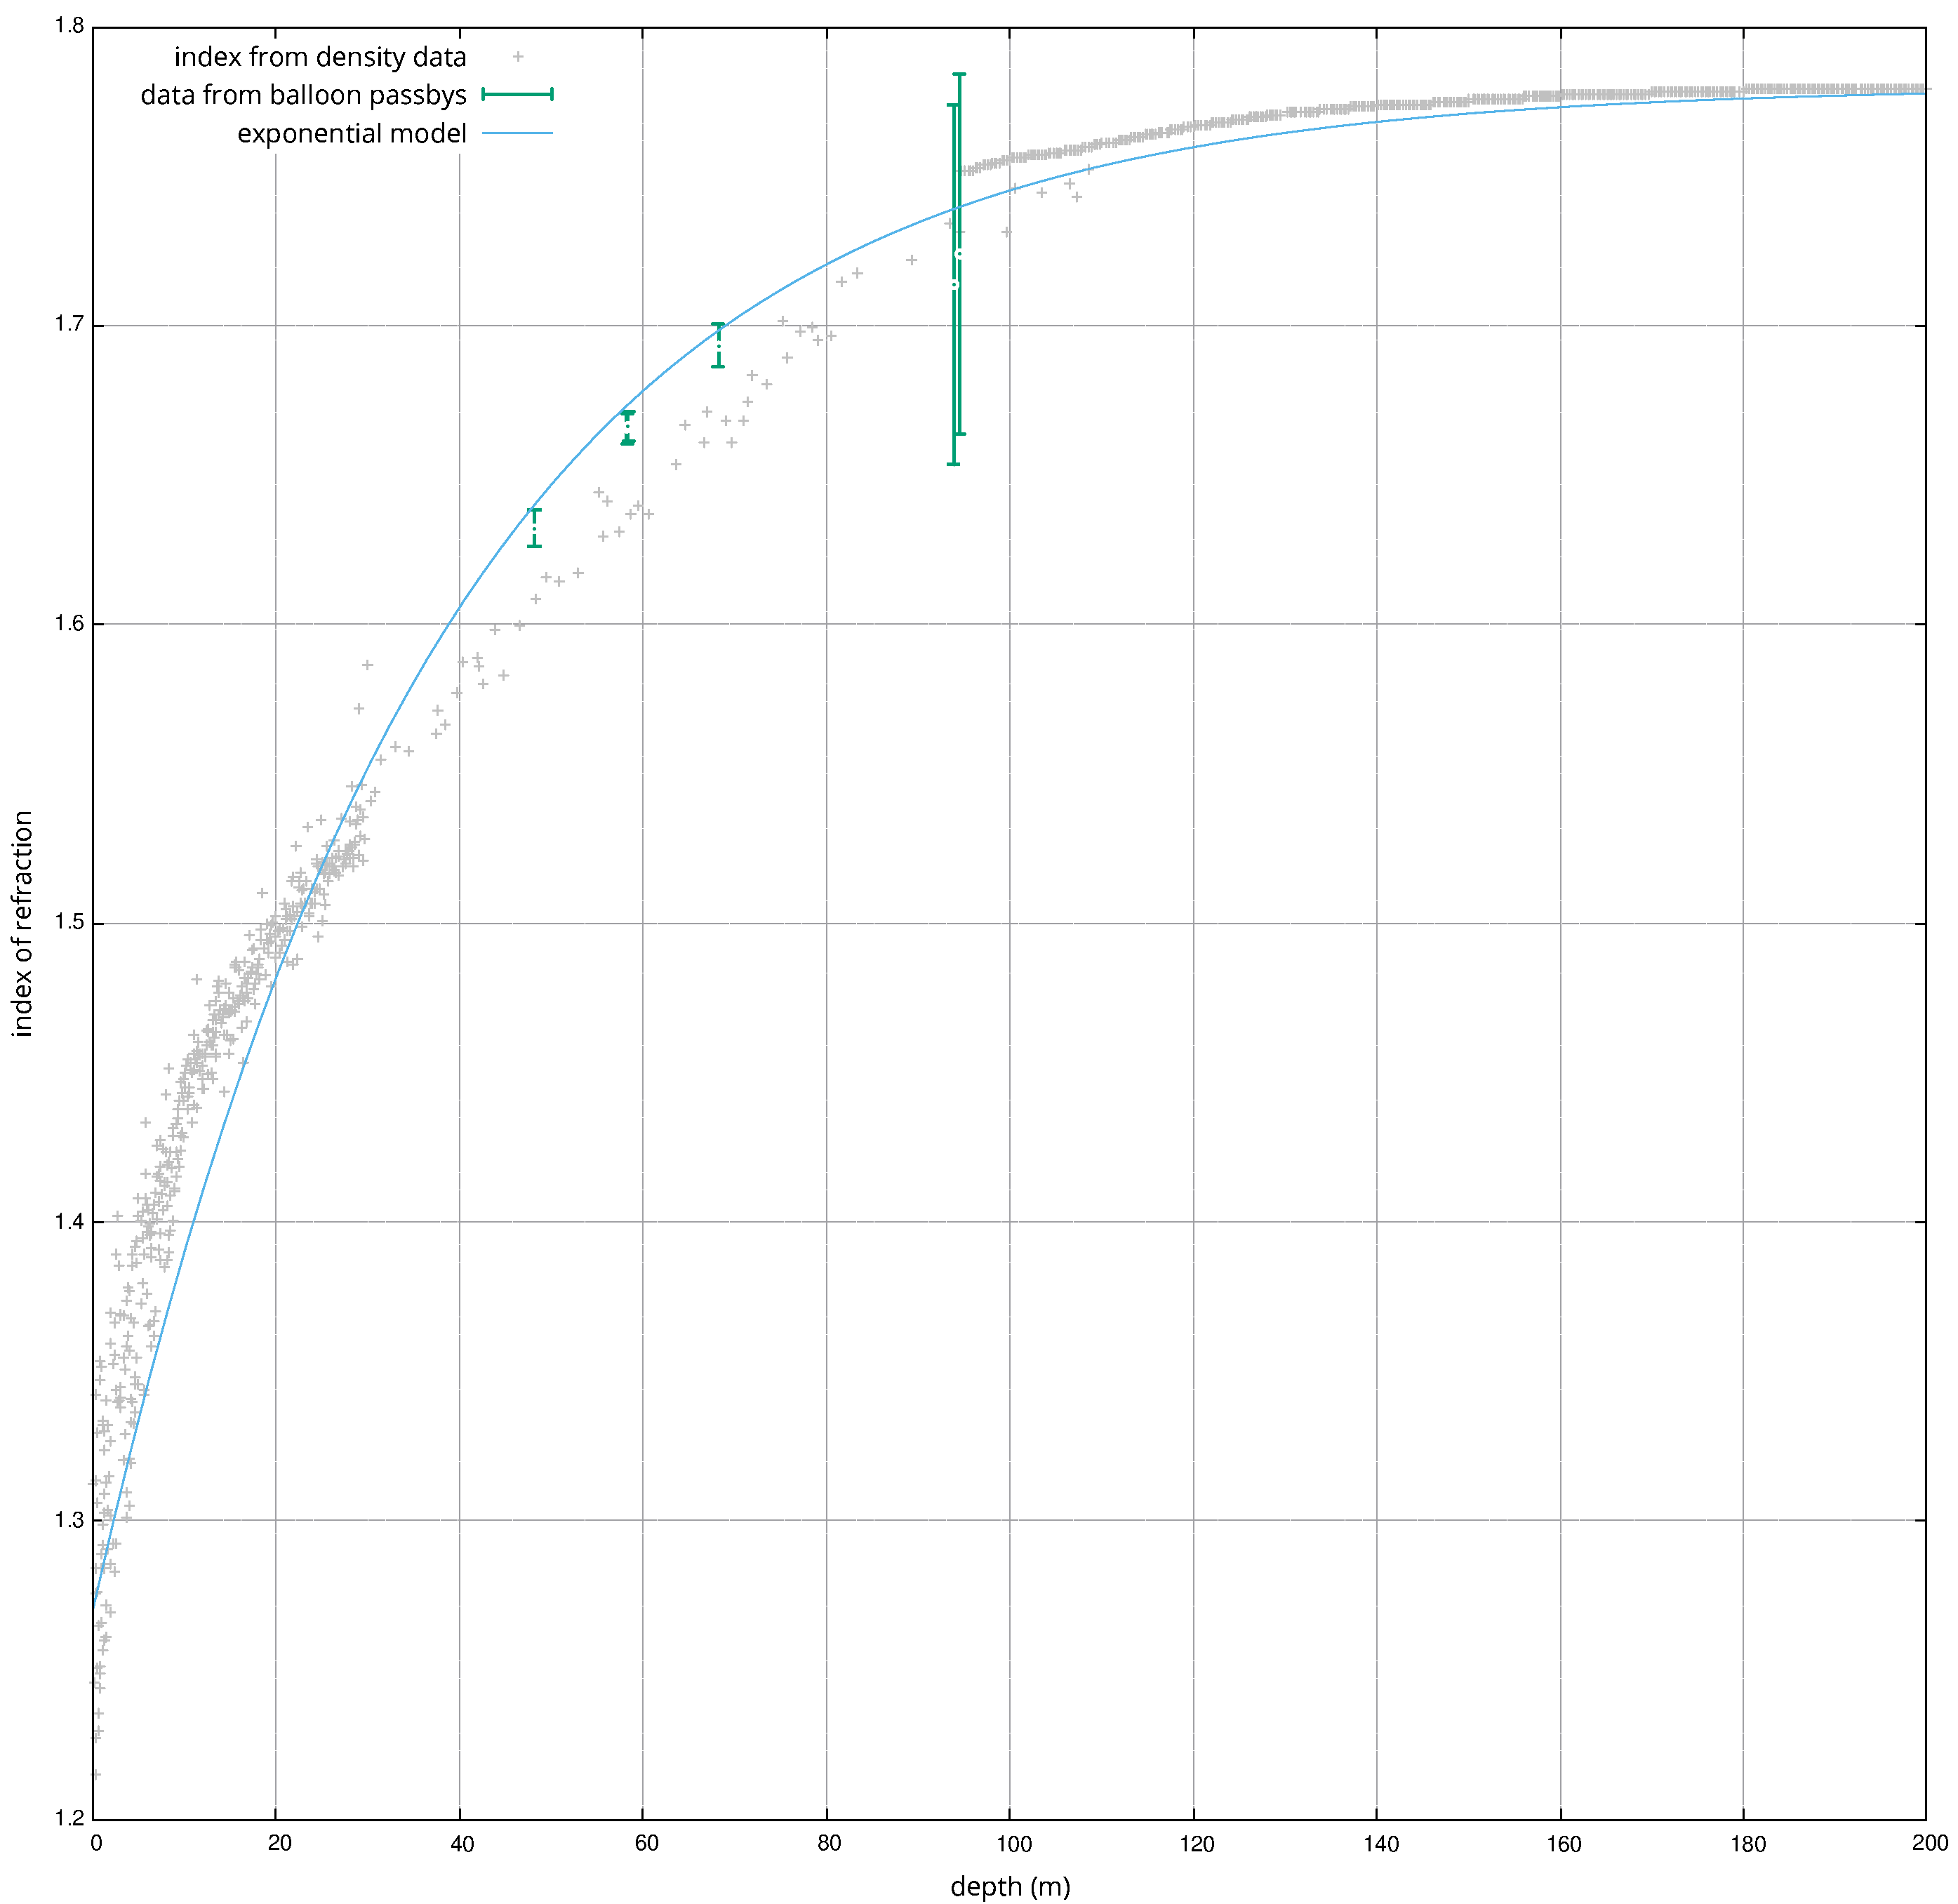
\includegraphics[width=\textwidth]{figures/ResultsBig.pdf}
  \caption{In this bigger plot it's easier to see just where our measured values lie}
	\label{fig:ResultsBig}
\end{figure}
\chapter{Balloon passbys under 5°\\ in the summer of 2022}
\label{app:5Deg}
\csvautotabular{tables/EventsBelow5DegPart1.csv}
\csvautotabular{tables/EventsBelow5DegPart2.csv}
\csvautotabular{tables/EventsBelow5DegPart3.csv}
\chapter{Balloon passbys under 10°\\ in the summer of 2022}
\label{app:10Deg}
\begin{table}[h!]
\csvautotabular{tables/EventsBelow10DegPart5.csv}
\end{table}
\begin{table}
\csvautotabular{tables/EventsBelow10DegPart1.csv}
\end{table}
\begin{table}
\csvautotabular{tables/EventsBelow10DegPart2.csv}
\end{table}
\begin{table}
\csvautotabular{tables/EventsBelow10DegPart3.csv}
\end{table}
\begin{table}
\csvautotabular{tables/EventsBelow10DegPart4.csv}
\end{table}


\bibliographystyleFig{IEEEtran}
\bibliographyFig{IEEEabrv,Bibliography/FigureSources}


\bibliographystyle{IEEEtran}
\bibliography{IEEEabrv,Bibliography/sources}

\end{document}
